{\pdfoutput=1
\documentclass[runningheads,a4paper]{llncs}

\usepackage{amssymb}
\usepackage{amsmath}
\setcounter{tocdepth}{3}
\usepackage{graphicx}
\usepackage{amsmath}
\usepackage{hyperref}
\usepackage{todonotes}
\usepackage{datetime}
\usepackage{listings}
\usepackage{xcolor}
\usepackage{wrapfig}
\usepackage{subfig}
\usepackage{booktabs}
\usepackage{url}
\usepackage{float}
\usepackage{upquote}

\renewcommand{\arraystretch}{1.3}

\newcommand{\todonoteinline}[1]{\todo[color=red!40,inline,caption={TODO}]{#1}}
\newcommand{\todonote}[1]{\todo[color=red!40,caption={TODO}]{#1}}

%\newcommand{\replocdir}{https://github.com/searchivarius/NonMetricSpaceLib/tree/master/}
%\newcommand{\replocfile}{https://github.com/searchivarius/NonMetricSpaceLib/blob/master/}

\newcommand{\replocdir}{https://github.com/searchivarius/NonMetricSpaceLib/tree/pserv}
\newcommand{\replocfile}{https://github.com/searchivarius/NonMetricSpaceLib/blob/pserv/}

\newcommand{\ttt}[1]{\texttt{#1}}
\newcommand{\knn}{$k$-NN }
\newcommand{\knnns}{$k$-NN}
\newcommand{\ED}{\mbox{\rm ED}}
\newcommand{\pos}{\mbox{\rm pos}}
\newcommand{\rev}{\mbox{\rm rev}}
\newcommand{\DEL}[2]{\Delta_{#1}(#2)}

\newcommand{\LibVersion}{1.5}

\setcounter{secnumdepth}{3}

\begin{document}

\mainmatter  % start of an individual contribution

% first the title is needed
\title{Non-Metric Space Library (NMSLIB) Manual}

% a short form should be given in case it is too long for the running head
\titlerunning{NMSLIB Manual}

% the name(s) of the author(s) follow(s) next
%
% NB: Chinese authors should write their first names(s) in front of
% their surnames. This ensures that the names appear correctly in
% the running heads and the author index.
%
\author{Bilegsaikhan Naidan\inst{1} \and Leonid Boytsov\inst{2}}
%
\authorrunning{Bilegsaikhan Naidan and Leonid Boytsov}
% (feature abused for this document to repeat the title also on left hand pages)

% the affiliations are given next; don't give your e-mail address
% unless you accept that it will be published
\institute{
Department of Computer and Information Science,\\
Norwegian University of Science and Technology,\\
Trondheim, Norway\\
{\hspace{1em}}\\
\and
Language Technologies Institute, \\
Carnegie Mellon University,\\
Pittsburgh, PA, USA\\
\email{srchvrs@cs.cmu.edu}\\
}

%
% NB: a more complex sample for affiliations and the mapping to the
% corresponding authors can be found in the file "llncs.dem"
% (search for the string "\mainmatter" where a contribution starts).
% "llncs.dem" accompanies the document class "llncs.cls".
%

%\toctitle{Lecture Notes in Computer Science}
%\tocauthor{Authors' Instructions}

\maketitle

{\begin{center}{\small \textbf{Maintainer}: Leonid Boytsov}\end{center}}
{\begin{center}{Version \LibVersion}\end{center} 
{\begin{center}{{\today}}\end{center}}

\begin{abstract}
This document describes a library for similarity searching.
Even though the library contains a variety of metric-space access methods,
our main focus is on search methods for non-metric spaces.
Because there are fewer exact solutions for non-metric spaces,
many of our methods give only approximate answers. 
Thus, the methods
are evaluated in terms of efficiency-effectiveness trade-offs
rather than merely in terms of their efficiency.
Our goal is, therefore, to provide
not only state-of-the-art approximate search methods for 
both non-metric and metric spaces,
but also the tools to measure search quality.
We concentrate on technical details, i.e., 
how to compile the code, run the benchmarks, evaluate results,
and use our code in other applications.
Additionally, we explain how to extend the code by adding
new search methods and spaces.
\end{abstract}

\section{Introduction}
\subsection{What's new in version \LibVersion{} (major changes)} 
\todonoteinline{This section needs to be re-worked and duplicated in README/log}
\begin{itemize}
\item We have improved performance of two core methods SW-graph and NAPP, see \ref{}\todonote{add references}
\item We have adopted a new method: a hierarchical (navigable) small-world graph (HNSW),
contributed by Yury Malkov \cite{Malkov2016}, see \ref{} \todonote{add a reference}
\item We have modified the workflow of our benchmarking utility \ttt{experiment}
and improved handling of the gold standard data, see \ref{} \todonote{add a reference};
\item We have updated the API so that methods can save and restore indices, see \ref{} \todonote{add a reference};
\item We have implemented a server, which can have clients in Java and Python, see \ref{}. 
\item Last, we removed methods \ttt{permutation}, \ttt{permutation\_incsort}, and \ttt{permutation\_vptree}. 
The latter two methods are superseded by \ttt{proj\_incsort} and \ttt{proj\_vptree}, respectively.
\end{itemize}

\subsection{History, Objectives, and Principles}
The Non-Metric Space Library (shortly NMSLIB) is a collection of
similarity search methods and a toolkit for their evaluation.
Our software suit can also be used as a standalone search library on Linux and Windows. 
Most search methods were implemented by Bileg(saikhan) Naidan and Leo(nid) Boytsov.\footnote{Leo(nid) Boytsov is a maintainer.}
Additional contributors are listed on the \href{https://github.com/searchivarius/NonMetricSpaceLib}{GitHub 
page}.
Bileg and Leo gratefully acknowledge support by the iAd Center~\footnote{\url{http://www.iad-center.com/}}
and the Open Advancement of Question Answering Systems (OAQA) group~\footnote{\url{http://oaqa.github.io/}}.

%We encourage potential users and contributors to use GitHub for bug reports.

The code written by Bileg and Leo is distributed under the business-friendly \href{http://apache.org/licenses/LICENSE-2.0}{Apache License}. 
However, some third-party contributions are licensed differently.
For more information regarding licensing and acknowledging the use of the library
resource, please refer to \S~\ref{SectionCredits}.

The design of the library was influenced by 
and superficially resembles the design of the Metric Spaces Library \cite{LibMetricSpace}.
Yet our approach is different in many ways:

\begin{itemize}
\item We focus on approximate\footnote{
An approximate method may not
return a true nearest-neighbor or
 all the points within a given query ball.}
  search methods and non-metric spaces.

\item We simplify experimentation, in particular, 
through automatically measuring and aggregating important parameters
related to speed, accuracy, index size, and index creation time. 
In addition, we provide capabilities for testing in both single- and multi-threaded modes
to ensure that implemented solutions scale well with the number of available CPUs.

\item We care about overall efficiency and
aim to implement methods that have runtime comparable to an optimized production system. 
\end{itemize}

Search methods for non-metric spaces are especially interesting.
This domain does not provide sufficiently generic \emph{exact} search methods.
We may know very little about analytical properties of the distance
or the analytical representation may not be available at all (e.g., if the 
distance is computed by a black-box device \cite{Skopal:2007}).
In many cases it is not possible to search exactly
and instead one has to resort to approximate search procedures.

This is why methods
are evaluated in terms of efficiency-effectiveness trade-offs
rather than merely in terms of their efficiency.
We suspect that there is no ``one-size-fits-all'' search method.
Therefore, it is important to provide a variety of methods
each of which may work best for some specific classes of data.

Our commitment to efficiency affected several design decisions:
\begin{itemize}
\item The library is implemented in C++;
\item We focus on in-memory indices 
and, thus, do not require our methods to materialize a disk-based version of an index
(this also reduces programming effort).
However, one of our immediate goals is to support serialization of several best methods.
%It is, nevertheless, possible to benchmark disk-based implementations as well (see \ref{SectionWorkflow}).

\item 
We provide efficient implementations of many distance functions,
which rely on Single Instruction Multiple Data (SIMD) CPU commands  and/or
approximation of computationally intensive mathematical operations (see \S~\ref{SectionEfficiency}). 
\end{itemize}

It is often possible to demonstrate a substantial reduction in the number of distance computations
compared to sequential searching.
However, such reductions may entail additional computations (i.e., extra book-keeping)
and do not always lead to improved overall performance \cite{Boytsov_and_Bilegsaikhan:sisap2013}.
To eliminate situations where book-keeping costs are ``masked''
by inefficiencies of the distance function,
we pay special attention to distance function efficiency.

\subsection{Problem Formulation}
Similarity search is an essential part of many applications,
which include, among others,  
content-based retrieval of multimedia  and statistical machine learning.
The search is carried out in a finite database of objects $\{o_i\}$,
using a search query $q$ and a dissimilarity measure (the term data point or simply a point is often
used a synonym to denote either a data object or a query).
The dissimilarity measure is typically represented by a distance function $d(o_i, q)$. 
The ultimate goal is to answer a query by retrieving a subset of database objects sufficiently similar to the query $q$.
These objects will be called \emph{answers}.
Note that we use the terms \emph{distance} and the \emph{distance function} in a broader sense than
some of the textbooks:
We do not assume that the distance is a true metric distance. 
The distance function can disobey the triangle inequality and/or be even non-symmetric.

Two retrieval tasks are typically considered: a nearest neighbor and a range search. 
The nearest neighbor search aims to find the least dissimilar object,
i.e., the object at the smallest distance from the query.
Its direct generalization is the $k$-nearest neighbor search (the \knn search),
which looks for the $k$ most closest objects.
Given a radius $r$, 
the range query retrieves all objects within a query ball (centered at the query object $q$) with the radius $r$,
or, formally, all the objects~$\lbrace o_i \rbrace$ such that $d(o_i, q) \le r$. 
In generic spaces, the distance is not necessarily symmetric. 
Thus, two types of queries can be considered. 
In a  \emph{left} query, the object is the left argument of the distance function,
while the query is the right argument.
In a \emph{right} query, $q$ is the first argument and the object is the second, i.e.,
the right, argument.

The queries can be answered either exactly, 
i.e., by returning a complete result set that does not contain erroneous elements, or, 
approximately, e.g., by finding only some answers.
Thus, the methods are evaluated in terms of efficiency-effectiveness trade-offs
rather than merely in terms of their efficiency.
One common effectiveness metric is recall. In the case
of the nearest neighbor search, it is computed as
an average fraction of true neighbors returned by the method.
If ground-truth judgements (produced by humans) are available,
it is also possible to compute an accuracy of a \knn based classification
(see \S~\ref{SectionEffect}).

%In the current release, we focus on vector-space implementations,
%i.e., all the distance functions are defined over real-valued vectors. 
%Note that this is not a principal limitation, 
%because most methods do not access data objects
%directly. 
%Instead, they rely only on distance values.
%In the future, we plan to add more complex spaces, in particular, string-based.

\section{Getting Started}
\subsection{Prerequisites}
NMSLIB was developed and tested on 64-bit Linux.
Yet, almost all the code can be built and run on 64-bit Windows (two notable exceptions are: LSHKIT and NN-Descent).
It should also be possible to build the library on MAC OS.
Building the code requires a modern C++ compiler that supports \mbox{C++11}.
Currently, we support GNU C++ ($\ge4.7$), Intel compiler ($\ge14$), 
Clang ($\ge3.4$), 
and Visual Studio ($\ge12$)\footnote{One can use the free express version.}.
Under Linux, the build process relies on CMake. 
Under Windows, one could use Visual Studio projects stored in the repository.
These projects are for Visual Studio 14 (2015). 
However, they can be downgraded to work with Visual Studio 12 (see \S~\ref{SectionBuildWindows}).

%Note, however, that we do not have a portable code to measure memory consumption:
%This part will work only for Linux (with \href{https://en.wikipedia.org/wiki/Procfs}{PROCFS})
%and Windows. 

More specifically, for Linux we require:
\begin{enumerate}
\item A \textbf{64-bit} distributive (Ubuntu \textbf{LTS} is recommended)
\item GNU C++ ($\ge4.7$), Intel Compiler ($\ge14$), Clang ($\ge3.4$)
\item CMake (GNU make is also required)
\item Boost (dev version $\ge48$, Ubuntu package \ttt{libboost1.48-all-dev})
\item GNU scientific library (dev version, Ubuntu package \ttt{libgsl0-dev})
\item Eigen (dev version, Ubuntu package \ttt{libeigen3-dev})
\end{enumerate}

For Windows, we require:
\begin{enumerate}
\item A \textbf{64-bit} distributive (we tested on Windows 8); 
\item Visual Studio Express (or Professional) version 12 or later;
\item Boost is not required to build the core library and test utilities, 
but it is necessary to build some applications,
including the main testing binary \ttt{experiment.exe} (see \S~\ref{SectionBuildWindows}). 
\end{enumerate}

Efficient implementations of many distance functions (see \S~\ref{SectionEfficiency})
rely on SIMD instructions,
which operate on small  vectors of integer or floating point numbers. 
These instructions are available on most modern processors,
but we support only SIMD instructions available on recent Intel and AMD processors.   
Each distance function has a pure C++ implementation,
which can be less efficient than an optimized SIMD-based implementation.

On Linux, SIMD-based implementations are activated automatically 
for all sufficiently recent CPUs. 
On Windows, only SSE2 is enabled by default\footnote{Because SSE2 is available on all 64-bit computers.}. 
Yet, it is necessary to manually update project settings 
to enable more recent SIMD extensions (see \S\ref{SectionBuildWindows}).

Scripts to generate and process data sets are written in Python.
We also provide a sample Python script to plot performance graphs: \href{\replocfile sample_scripts/sample_scripts/genplot.py}{genplot.py} (see \S~\ref{SectionGenPlot}).
In addition to Python, this plotting script requires Latex and PGF. 

\subsection{Installing C++11 Compilers}
Installing C++11 compilers can be tricky, 
because they are not always provided as a standard package.
This is why we briefly review the installation process here. 
In addition, installing compilers does 
not necessarily make them default compilers.
One way to fix this is on Linux is to set environment variables \ttt{CXX} and \ttt{CC}.
For the GNU 4.7 compiler:
\begin{verbatim}
export CXX=g++-4.7 CC=gcc-4.7 
\end{verbatim}
For the Clang compiler:
\begin{verbatim}
export CXX=clang++-3.4 CC=clang-3.4
\end{verbatim}
For the Intel compiler:
\begin{verbatim}
export CXX=icc CC=icc 
\end{verbatim}

It is, perhaps, the easiest to obtain Visual Studio by simply downloading
it from the \href{https://www.microsoft.com/en-us/download/default.aspx}{Microsoft web-site}.
We were able to build and run the 64-bit code using the free distributive of Visual Studio Express 14 (also called 
\ttt{Express 2015}) and Visual Studio 12 (Express 2013). The professional (and expensive) version of Visual Studio is not required. 


To install GNU C++ version 4.7 on newer Linux distributions (in particular, on Ubuntu 14) with the Debian package management system, 
one can simply type:
\begin{verbatim}
sudo apt-get install gcc-4.7 g++-4.7
\end{verbatim}
At the time of this writing, GNU C++ 4.8 was available as a standard package as well.


However, this would not work on older distributives of Linux. 
One may need to use an experimental repository as follows:
\begin{verbatim}
sudo add-apt-repository ppa:ubuntu-toolchain-r/test
sudo apt-get update
sudo apt-get install gcc-4.7 g++-4.7
\end{verbatim}
If the script \ttt{add-apt-repository} is missing, it can be installed as follows:
\begin{verbatim}
sudo apt-get install python-software-properties
\end{verbatim}
More details can be found on the \href{http://askubuntu.com/questions/113291/how-do-i-install-gcc-4-7}{AskUbuntu web-site.}

Similarly to the GNU C++ compiler, to install a C++11 version of Clang on newer Debian-based distributives one can simply type:
\begin{verbatim}
sudo apt-get install clang-3.6
\end{verbatim}

However, for older distributives one may need to add a non-standard repository.
For Debian and Ubuntu distributions, it is easiest to add repositories from \href{http://llvm.org/apt/}{the LLVM web-site}. 
For example, if you have Ubuntu 12 (Precise), you need to add repositories
as follows:\footnote{Do not forget to remove \ttt{deb-src} for source repositories.
See the discussion \href{http://askubuntu.com/questions/160511/why-does-add-apt-repository-fail-to-add-source-repositories}{here for more details.}}
\begin{verbatim}
sudo add-apt-repository \
  "deb http://llvm.org/apt/precise/ llvm-toolchain-precise main"
sudo add-apt-repository \
  "http://llvm.org/apt/precise/ llvm-toolchain-precise main"
sudo add-apt-repository \
  "deb http://llvm.org/apt/precise/ llvm-toolchain-precise-3.4 main"
sudo add-apt-repository \
  "http://llvm.org/apt/precise/ llvm-toolchain-precise-3.4 main"
sudo add-apt-repository \
  "deb http://ppa.launchpad.net/ubuntu-toolchain-r/test/ubuntu \
                                                  precise main"
\end{verbatim}
Then, Clang 3.4 (and LLDB debugger) can be installed by typing:
\begin{verbatim}
sudo apt-get install clang-3.4 lldb-3.4
\end{verbatim}

The Intel compiler can be freely used for non-commercial purposes by some categories of users (students, academics,
and active open-source contributors).
It is a part of C++ Composer XE for Linux and can 
be obtained \href{http://software.intel.com/en-us/non-commercial-software-development}{from the Intel web site}.
After downloading and running an installation script, one needs to set environment variables.
If the compiler is installed to the folder \ttt{/opt/intel}, environment variables
are set by a script as follows:
\begin{verbatim}
/opt/intel/bin/compilervars.sh intel64
\end{verbatim}



\subsection{Quick Start on Linux}\label{QuickStartLinux}
To build the project, go to the directory \href{\replocdir similarity_search}{similarity\_search} and type:  
\begin{verbatim}
cmake .  
make   
\end{verbatim}
This creates several binaries in the directory \ttt{similarity\_search/release}, 
most importantly, 
a benchmarking utility \ttt{experiment}, which carries out experiments,
and testing utilities \ttt{bunit}, \ttt{test\_integer}, and \ttt{bench\_distfunc}.
A more detailed description of the build process on Linux is given in \S~\ref{SectionBuildLinux}.

Examples of using the benchmarking utility can be found in the directory \href{\replocdir sample_scripts}{sample\_scripts}. 
Please, check the script \href{\replocfile sample_scripts/sample_run.sh}{sample\_run.sh}. 
The latter runs a bunch of methods. It can also create an efficiency-effectiveness plot if needed.



\subsection{Python bindings (only on Linux)}
We provide basic Python bindings (for Linux and Python 2.7). 
%\href{https://github.com/erikbern/ann-benchmarks}{One public evaluation of our library using these bindings was carried out by Erik Bernhardsson}. 


To build bindings for dense vector spaces (see \S~\ref{SectionSpaces} for the description of spaces), build the library first.
Then, change the directory to \ttt{python\_vect\_bindings} and type:
\begin{verbatim}
make
sudo make install
\end{verbatim} 
For an example of using our library in Python, see the script  \href{\replocfile python_vect_bindings/test_nmslib_vect.py}{test\_nmslib\_vect.py}.

Generic vector spaces are supported as well (see the directory \ttt{python\_gen\_bindings}. However, they work only for spaces
that properly define define serialization and de-serialization, see \S~\ref{} for details. \todo{Add a proper reference}

\subsection{Query server (only on Linux)}
\todonoteinline{Add a description, also update the README}

\subsection{Quick Start on Windows}\label{QuickStartWindows}
Building on Windows is straightforward.
Download \href{https://www.visualstudio.com/en-us/downloads/download-visual-studio-vs.aspx}{Visual Studio 2015 Express for Desktop}. 
Download and install respective \href{http://sourceforge.net/projects/boost/files/boost-binaries/1.59.0/boost_1_59_0-msvc-14.0-64.exe/download}{Boost binaries}. Please, use the \textbf{default} installation directory on disk \ttt{c:} (otherwise, it will be necessary to update project files).

Afterwards, one can simply use the provided \href{\replocfile similarity_search/NonMetricSpaceLib.sln}{Visual Studio 
solution file}.
The solution file references several project (*.vcxproj) files: 
\href{\replocfile similarity_search/src/NonMetricSpaceLib.vcxproj}{NonMetricSpaceLib.vcxproj}
is the main project file that is used to build the library itself.
The output is stored in the folder \ttt{similarity\_search\textbackslash x64}.
A more detailed description of the build process on Windows is given in \S~\ref{SectionBuildWindows}.

Note that the core library, the test utilities,
 as well as examples of the standalone applications (projects \ttt{sample\_standalone\_app1}
and \ttt{sample\_standalone\_app2})
can be built without installing Boost. 


\section{Building and running the code (in detail)}

A build process creates several important binaries, which include:

\begin{itemize}
\item NMSLIB library (on Linux \ttt{libNonMetricSpaceLib.a}),
which can be used in external applications;
\item The main benchmarking utility \ttt{experiment} (\ttt{experiment.exe} on Windows) 
that carries out experiments and saves evaluation results;
\item A tuning utility \ttt{tune\_vptree} (\ttt{tune\_vptree.exe} on Windows) 
that finds optimal VP-tree parameters (see \S~\ref{SectionVPtree} and our paper for details \cite{Boytsov_and_Bilegsaikhan:nips2013});
\item A semi unit test utility \ttt{bunit} (\ttt{bunit.exe} on Windows);
\item A utility \ttt{bench\_distfunc} that carries out integration tests (\ttt{bench\_distfunc.exe} on  Windows);
\end{itemize}

A build process is different under Linux and Windows. 
In  the following sections, we consider these differences in more detail. 

\subsection{Building under Linux}\label{SectionBuildLinux}
Implementation of similarity search methods is in the directory \ttt{similarity\_search}.
The code is built using a \ttt{cmake}, which works on top of the GNU make.
Before creating the makefiles, we need to ensure that a right compiler is used.
This is done by setting two environment variables: \ttt{CXX} and \ttt{CC}.
In the case of GNU C++ (version 4.7), you may need to type:
\begin{verbatim}
export CCX=g++-4.7 CC=gcc-4.7 
\end{verbatim}
In the case of the Intel compiler, you may need to type:
\begin{verbatim}
export CXX=icc CC=icc 
\end{verbatim}
If you do not set variables \ttt{CXX} and \ttt{CC}, 
the default C++ compiler is used (which can be fine, if it is the right compiler already).


To create makefiles for a release version of the code, type:
\begin{verbatim}
cmake -DCMAKE_BUILD_TYPE=Release .
\end{verbatim}
If you did not create any makefiles before, you can shortcut by typing:
\begin{verbatim}
cmake . 
\end{verbatim}
To create makefiles for a debug version of the code, type:
\begin{verbatim}
cmake -DCMAKE_BUILD_TYPE=Debug .
\end{verbatim}
When makefiles are created, just type:
\begin{verbatim}
make
\end{verbatim}
If \ttt{cmake} complains about the wrong version of the GCC, 
it is most likely that you forgot to set the environment variables \ttt{CXX} and \ttt{CC} (as described above).
If this is the case, make these variables point to the correction version of the compiler.
\textbf{Important note:} 
do not forget to delete the \ttt{cmake} cache and make file, before recreating the makefiles.
For example, you can do the following (assuming the current directory is \ttt{similarity\_search}):
\begin{verbatim}
rm -rf `find . -name CMakeFiles` CMakeCache.txt
\end{verbatim}

Also note that, for some reason, \ttt{cmake} might sometimes ignore environmental variables \ttt{CXX} and \ttt{CC}.
In this unlikely case, you can specify the compiler directly through \ttt{cmake} arguments.
For example, in the case of the GNU C++ and the \ttt{Release} build, 
this can be done as follows:
\begin{verbatim}
cmake -DCMAKE_BUILD_TYPE=Release -DCMAKE_CXX_COMPILER=g++-4.7 \
-DCMAKE_GCC_COMPILER=gcc-4.7 CMAKE_CC_COMPILER=gcc-4.7 .
\end{verbatim} 

The build process creates several binaries. Most importantly,
the main benchmarking utility \ttt{experiment}.
The directory \ttt{similarity\_search/release} contains release versions of
these binaries. Debug versions are placed into the folder \ttt{similarity\_search/debug}.

\textbf{Important note:} a shortcut command:
\begin{verbatim}
cmake .
\end{verbatim} 
(re)-creates makefiles for the previously 
created build. When you type \ttt{cmake .} for the first time,
it creates release makefiles. However, if you create debug
makefiles and then type \ttt{cmake .}, 
this will not lead to creation of release makefiles! 

To use the library in external applications, which do not belong to the library repository,
one needs to install the library first.
Assume that an installation location is the folder \ttt{NonMetrLibRelease} in the
home directory. Then, the following commands do the trick:
\begin{verbatim}
cmake \
    -DCMAKE_INSTALL_PREFIX=$HOME/NonMetrLibRelease \
    -DCMAKE_BUILD_TYPE=Release .
make install
\end{verbatim}

A directory \href{\replocfile sample_standalone_app}{sample\_standalone\_app} 
contains two sample programs (see files 
\href{\replocfile sample_standalone_app/sample_standalone_app1.cc}{sample\_standalone\_app1.cc}
and
\href{\replocfile sample_standalone_app/sample_standalone_app2.cc}{sample\_standalone\_app2.cc})
that use NMSLIB binaries installed in the folder \ttt{\$HOME/NonMetrLibRelease}.

\subsubsection{Developing and Debugging on Linux}
There are several debuggers that can be employed.
Among them, some of the most popular are: \ttt{gdb} (a command line tool)
and a \ttt{ddd} (a GUI wrapper for gdb).
For users who prefer IDEs, one good and free option is Eclipse IDE for C/C++ developers.
It is not the same as Eclipse for Java and one needs 
to \href{http://www.eclipse.org/ide/}{download 
this version of Eclipse separately.}.
An even better option is, perhaps, \href{https://www.jetbrains.com/clion/}{CLion}. However, it is not free.\footnote{There are
a few categories of people, including students, who can ask for a free license, though.}

\begin{figure}
\centering
\caption{\label{FigEclipse1}Selecting an existing project to import}
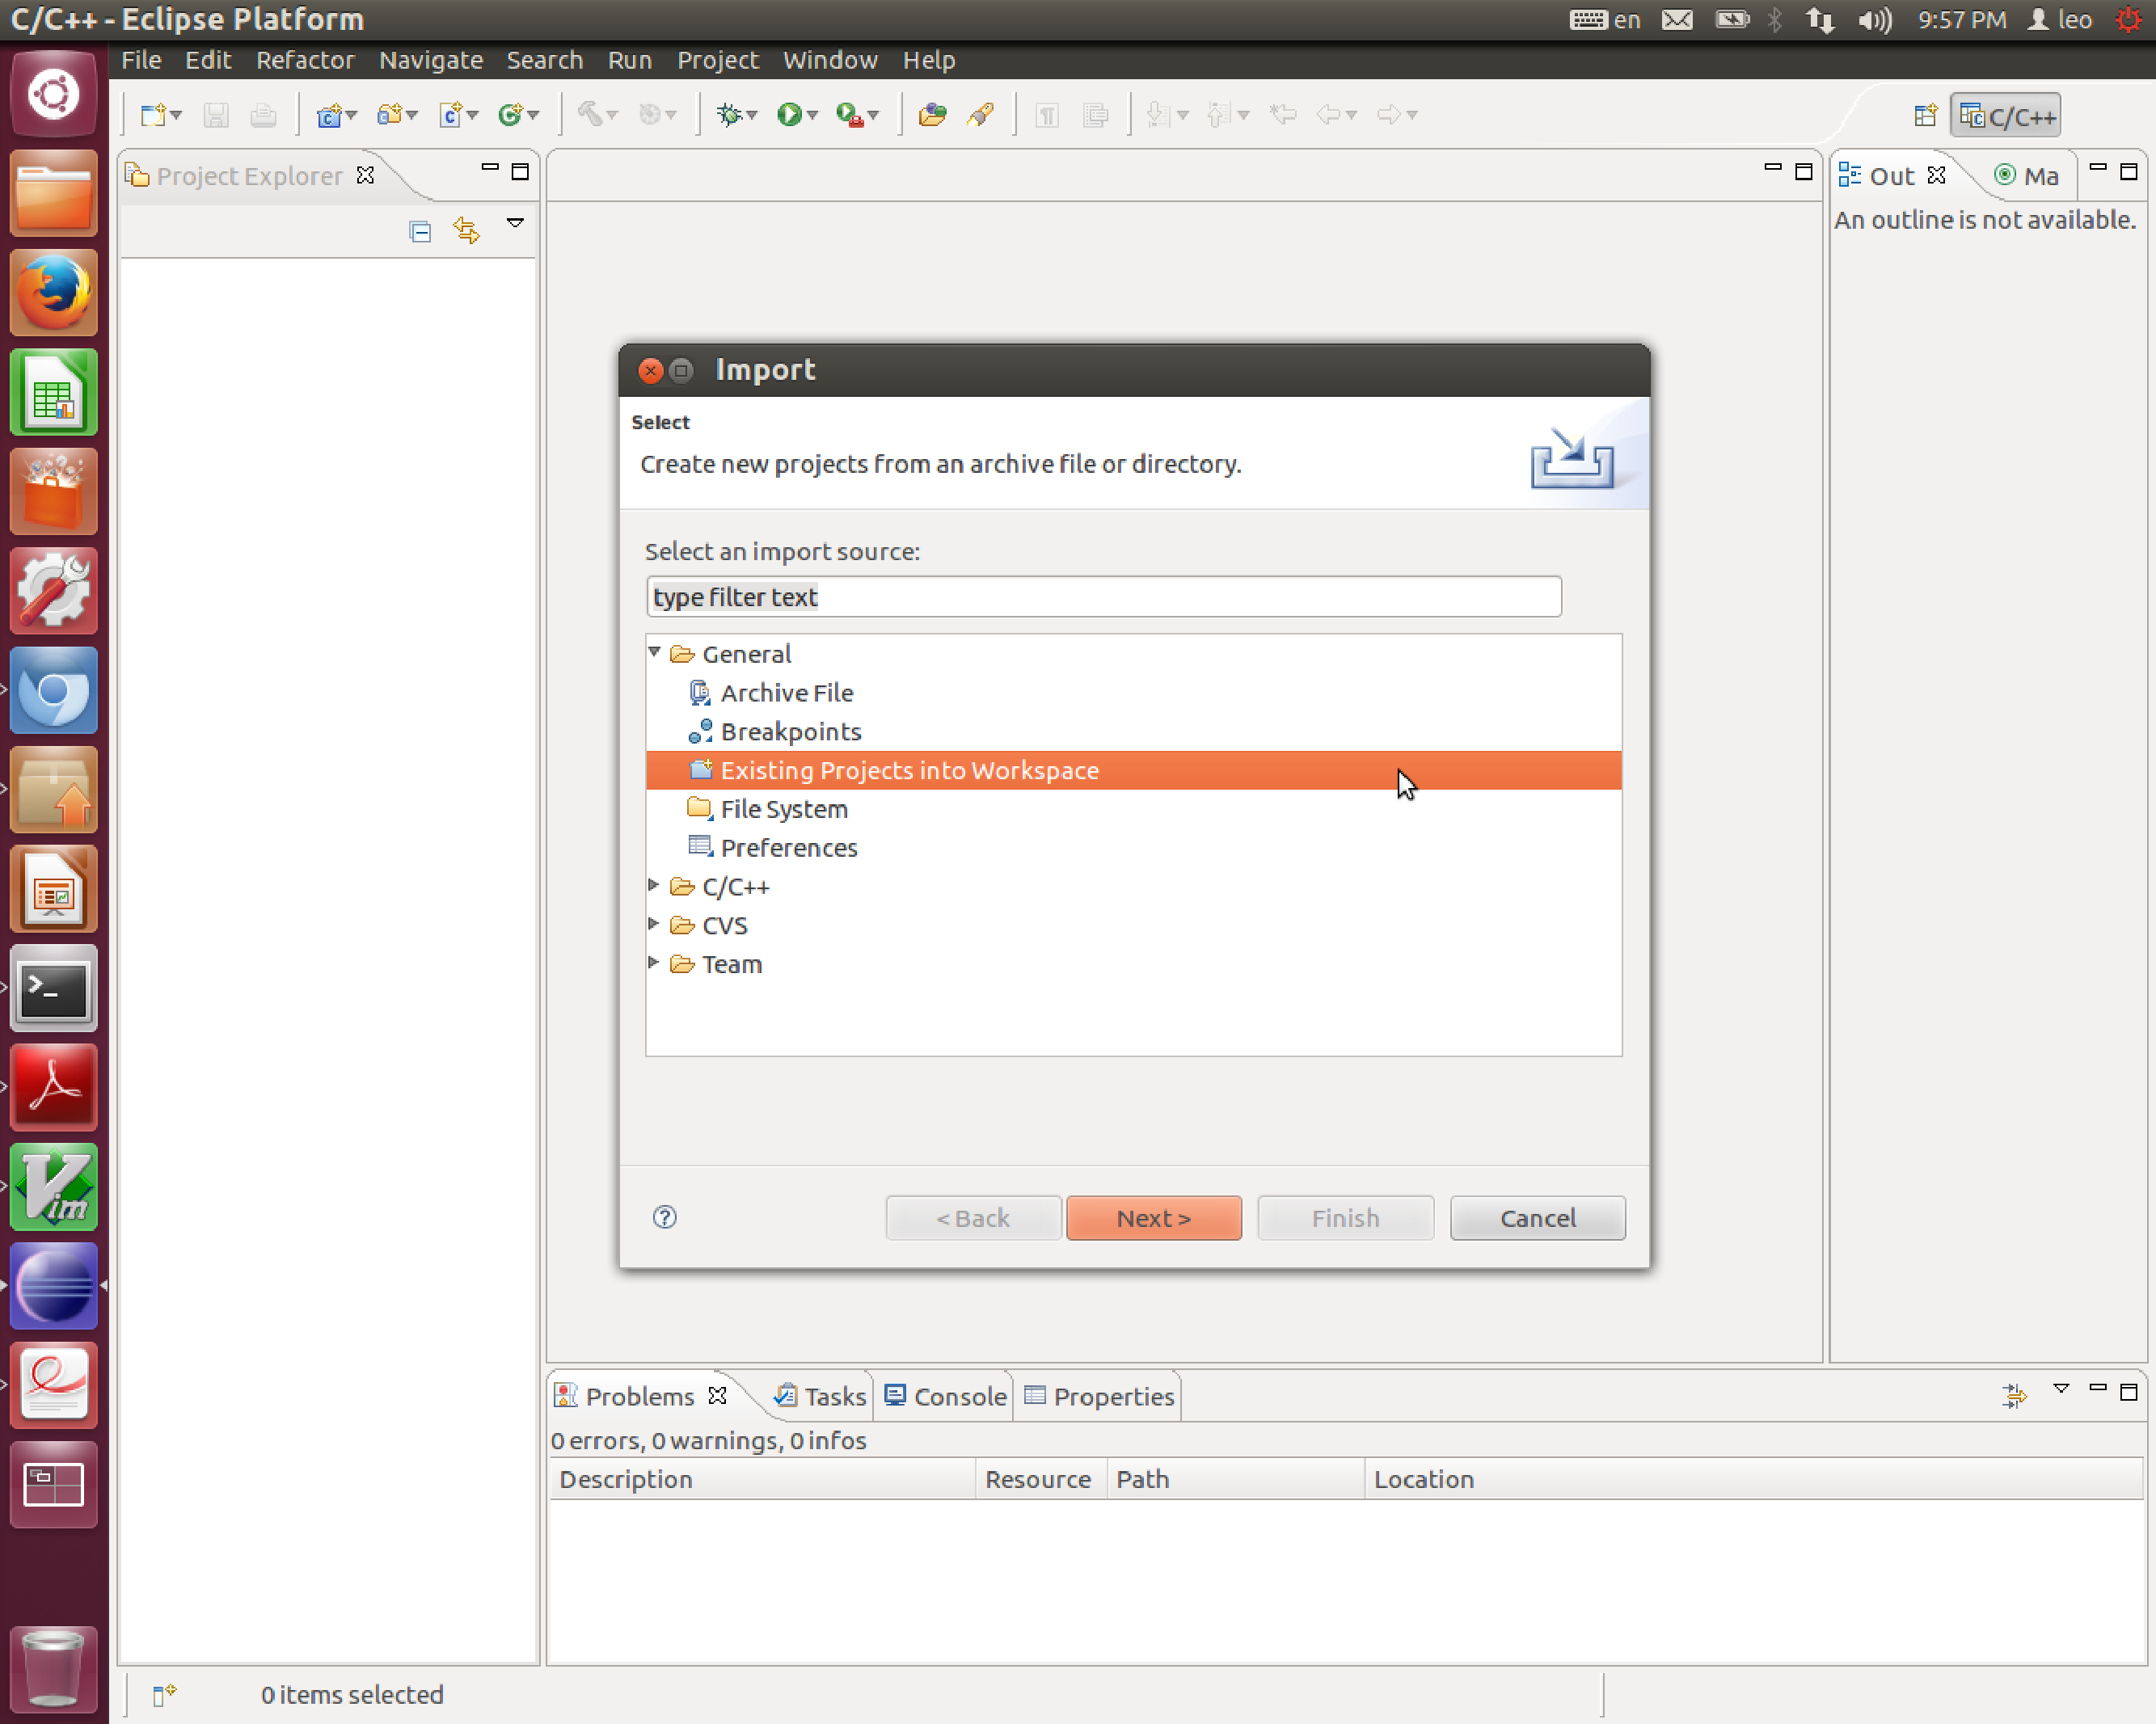
\includegraphics[width=0.9\textwidth]{figures/Eclipse1.pdf}
\end{figure}

After downloading and decompressing, e.g. as follows:
\begin{verbatim}
tar -zxvf eclipse-cpp-europa-winter-linux-gtk-x86_64.tar.gz
\end{verbatim}
one can simply run the binary \ttt{eclipse} (in a
newly created directory \ttt{eclipse}).
On the first start, Eclipse will ask you select a repository location.
This would be the place to store the project metadata and (optionally)
actual project source files.
The following description is given for Eclipse Europe. 
It may be a bit different with newer versions of Eclipse.


\begin{figure}
\centering
\caption{\label{FigEclipse2}Importing an existing project}
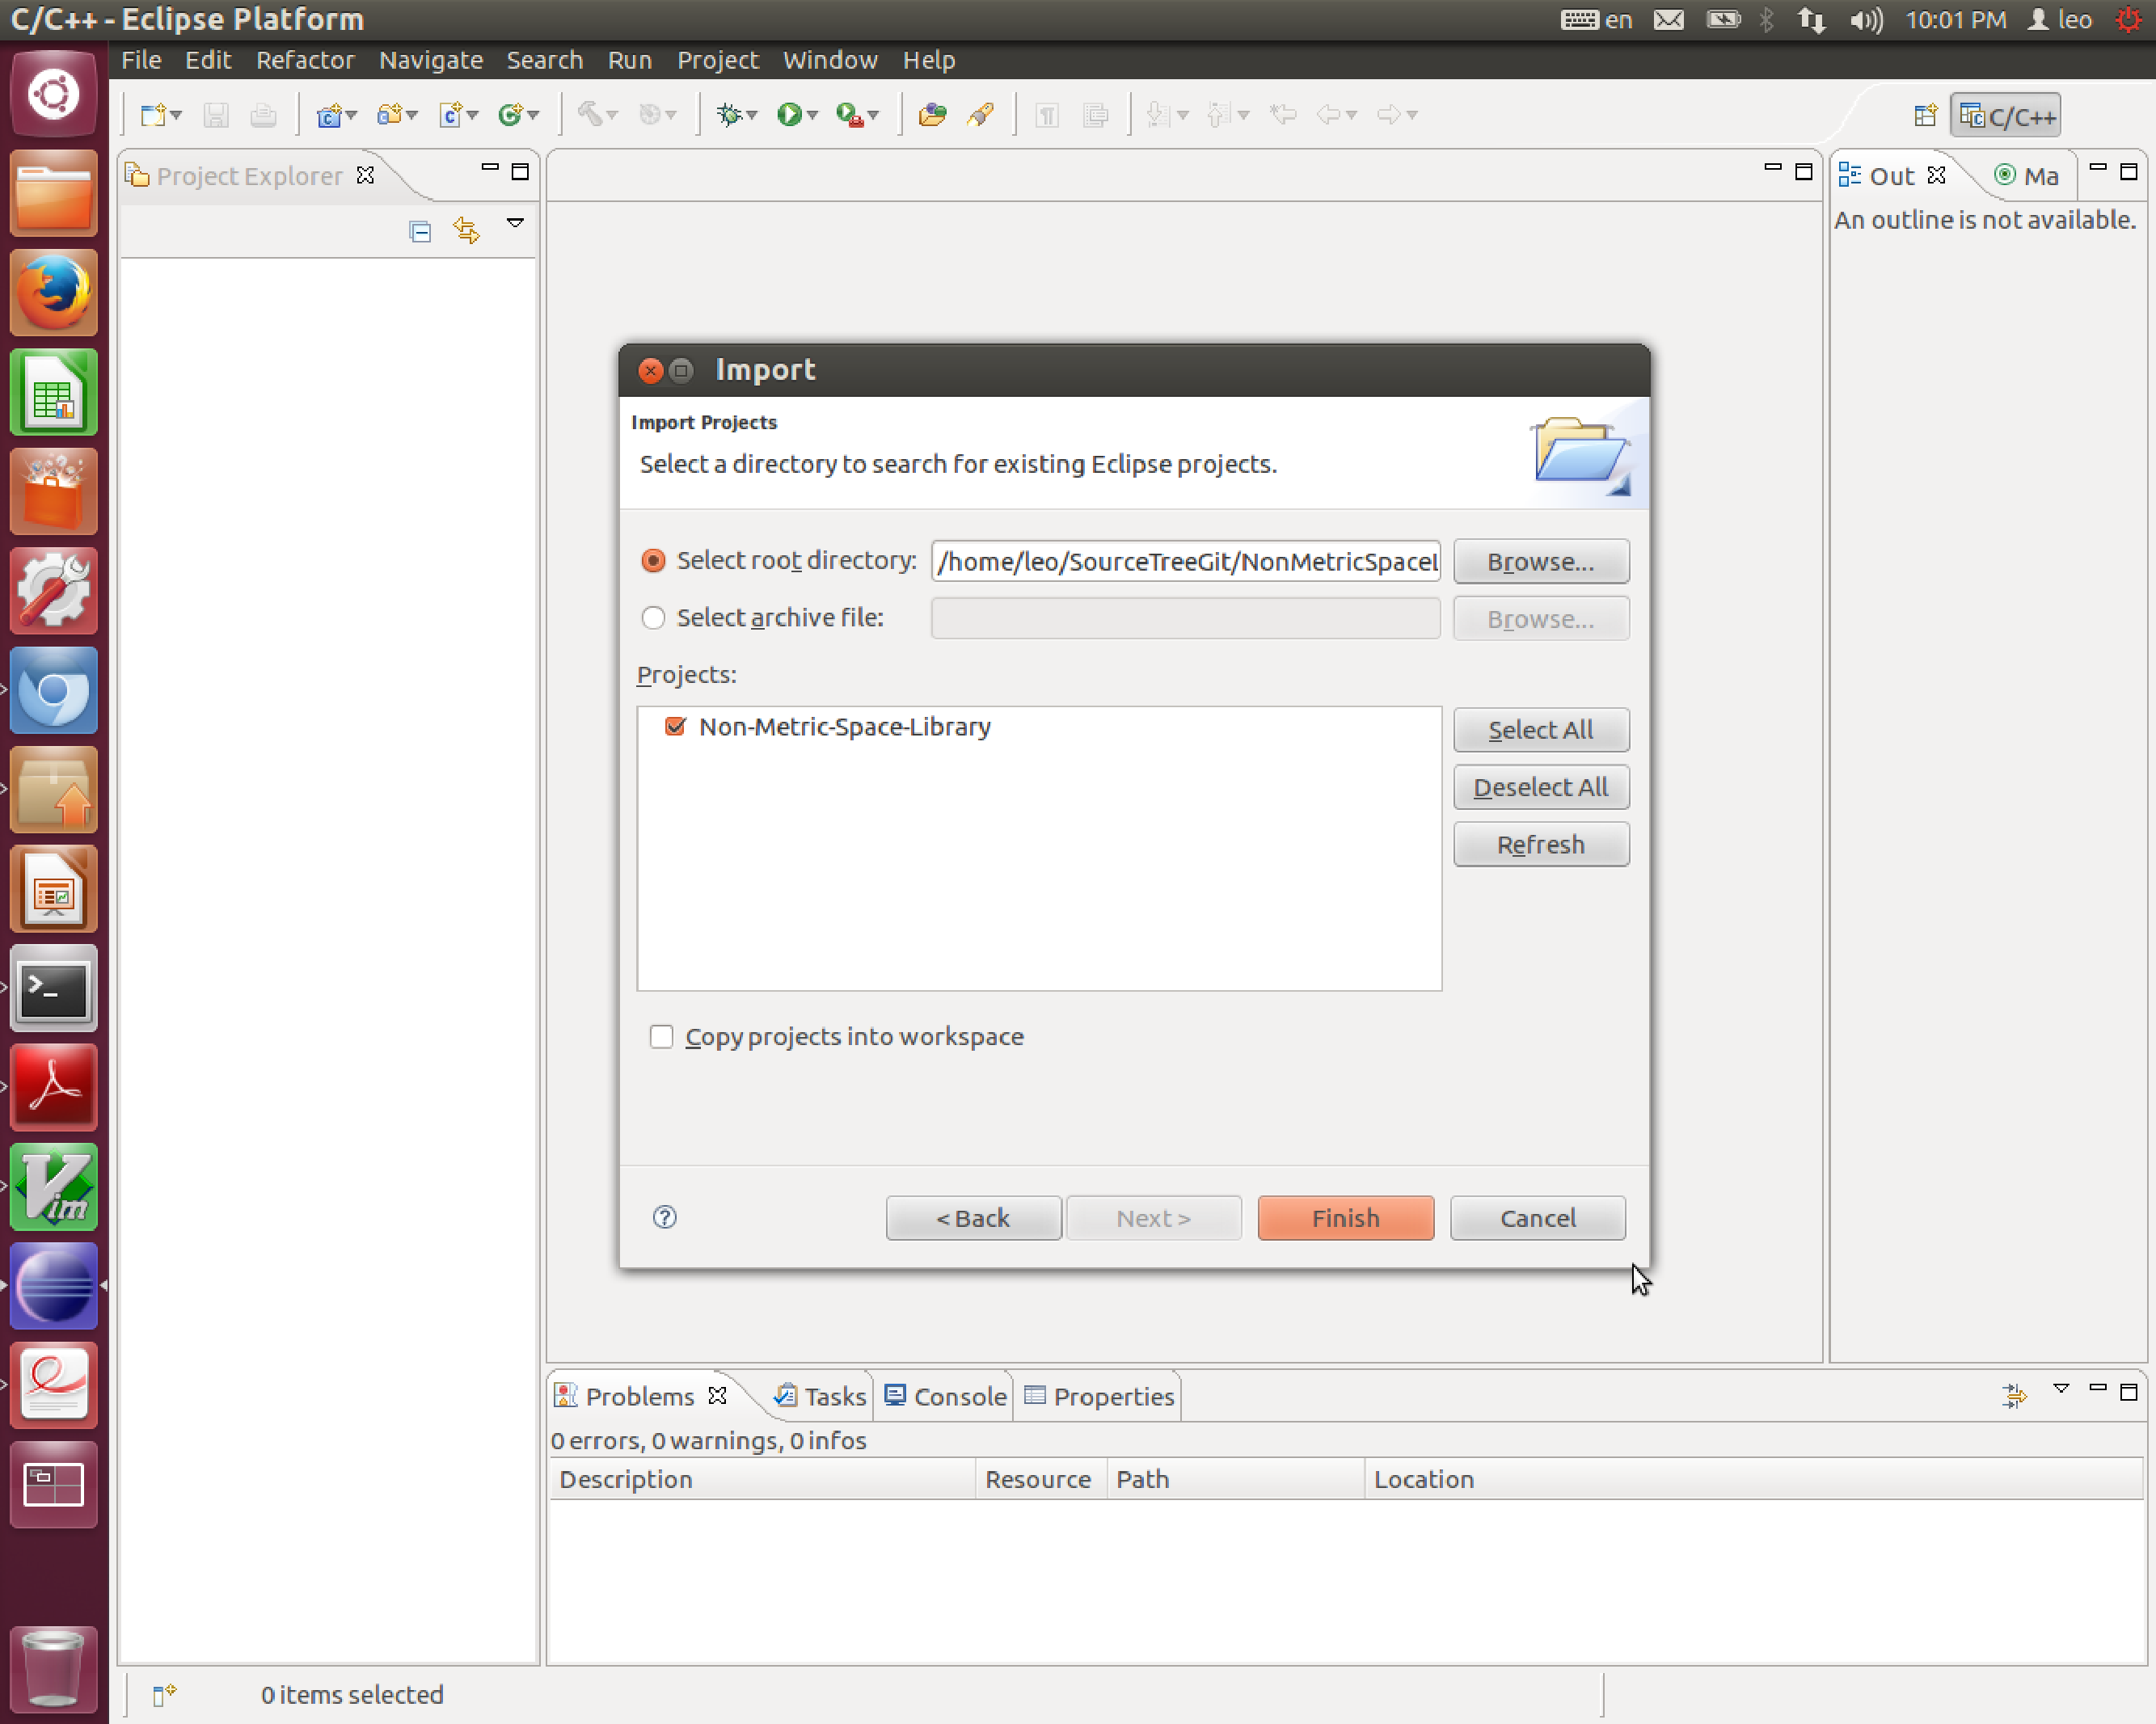
\includegraphics[width=0.9\textwidth]{figures/Eclipse2.pdf}
\end{figure}

After selecting the workspace, the user can import the Eclipse project
stored in the GitHub repository.
Go to the menu \ttt{File}, sub-menu \ttt{Import}, category \ttt{General} 
and choose to import
an existing project into the workspace as shown in Fig.~\ref{FigEclipse1}.
After that select a root directory. To this end,
go to the directory where you checked out the contents 
of the GitHub repository and enter a sub-directory \ttt{similarity\_search}.
You should now be able to see the project \ttt{Non-Metric-Space-Library}
as shown in Fig~\ref{FigEclipse2}.
You can now finalize the import by pressing the button \ttt{Finish}.

\begin{figure}
\centering
\caption{\label{FigEclipse3}Enabling indexing of the source code}
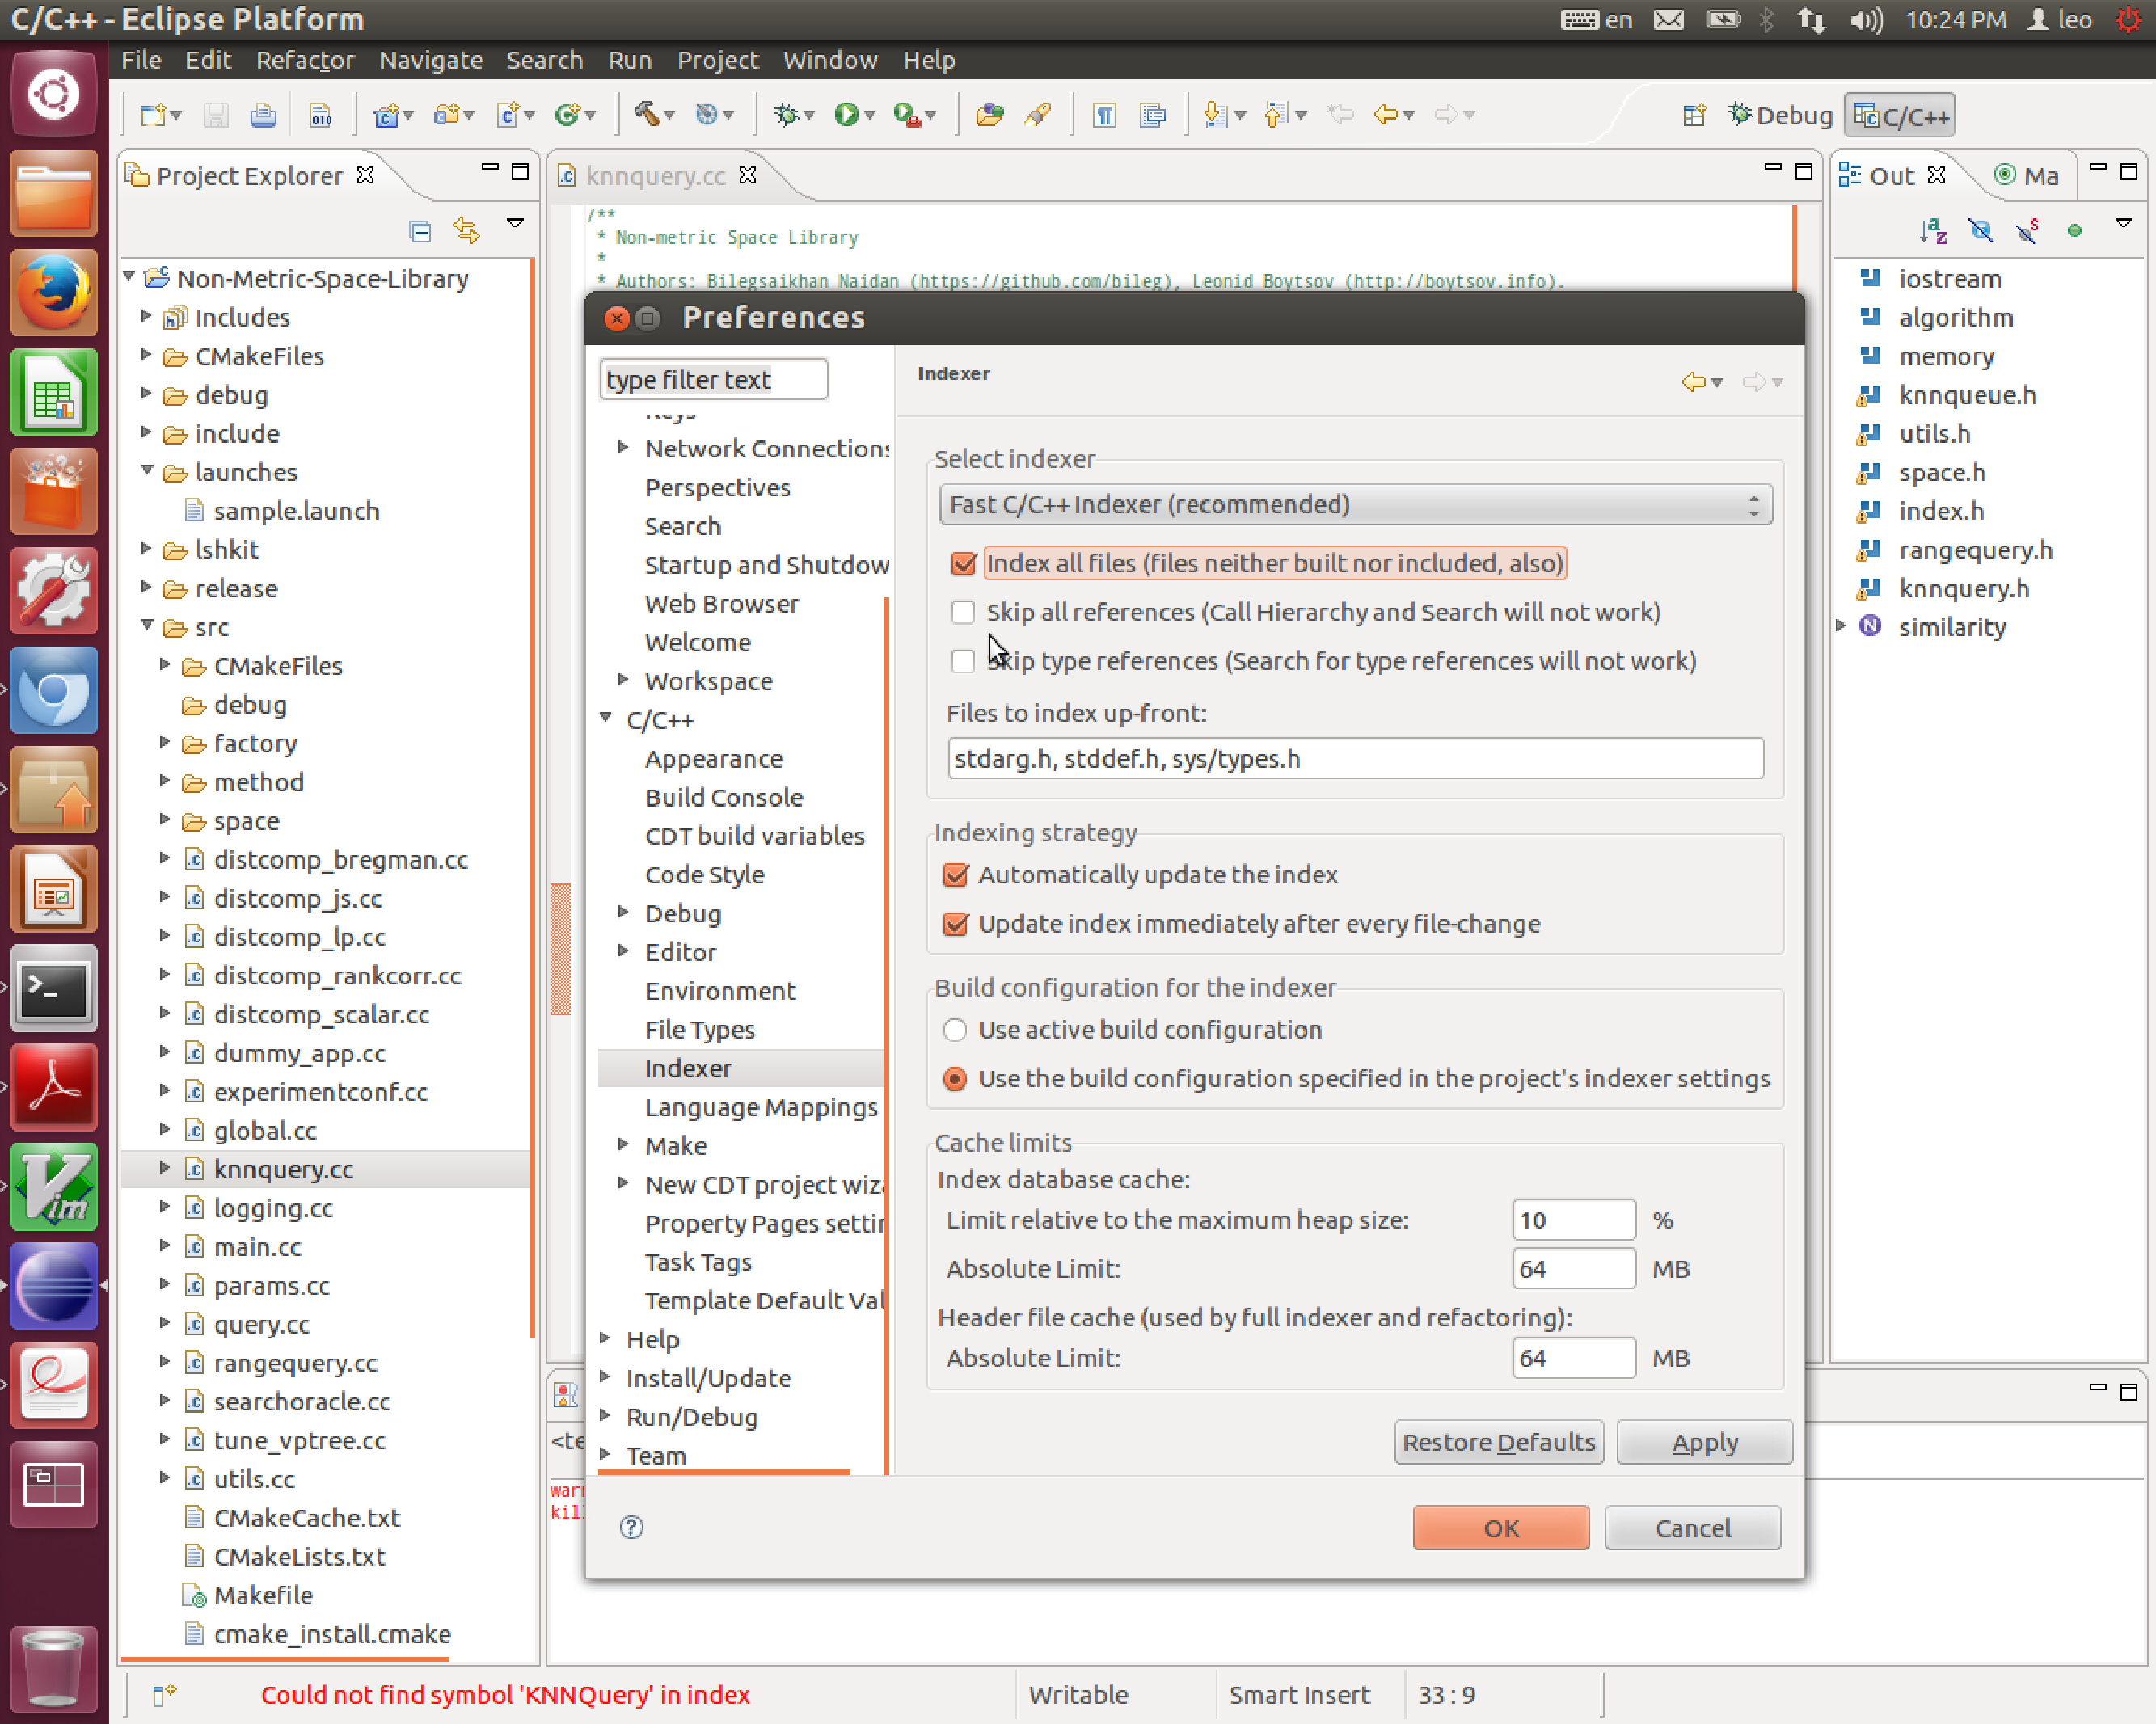
\includegraphics[width=0.9\textwidth]{figures/Eclipse3.pdf}
\end{figure}

Next, we need to set some useful settings.
Most importantly, we need to enable indexing of source files.
This would allow us to browse class hierarchies, as well as find declarations
of variables or classes.
To this end, go to the menu \ttt{Window}, sub-menu \ttt{Preferences}
and select a category \ttt{C++/indexing} (see Fig.~\ref{FigEclipse3}).
Then, check the box \ttt{Index all files}.
Eclipse will start indexing your files 
with the progress being shown in the status bar (right down corner).

The user can also change the editor settings. 
We would strongly encourage to disable the use of tabs.
Again, go the menu \ttt{Window}, sub-menu \ttt{Preferences},
and select a category \ttt{General/Editors/Text Editors}.
Then, check the box \ttt{Insert spaces for tabs}.
In the same menu, you can also change the fonts (use the
category \ttt{General/Appearance/Colors and Fonts}).

In a newer Eclipse version, disabling tabs is done differently. 
To this end, go to the menu \ttt{Window}, sub-menu \ttt{Preferences},
and select a category \ttt{C++/Code Style/Formatter}.
Then, you need to create a new profile and make this profile active. 
In the profile, change the tab policy to \ttt{Spaces only}. 

It is possible to build the project from Eclipse  (see the menu \ttt{Project}).
However, one first needs to generate makefiles as described in \S~\ref{SectionBuildLinux}.
The current limitation is that you can build either release
or the debug version at a time.
Moreover, to switch from one version to another, you need to recreate
the makefiles from the command line.

\begin{figure}
\centering
\caption{\label{FigDebugConf}Creating a debug/run configuration}
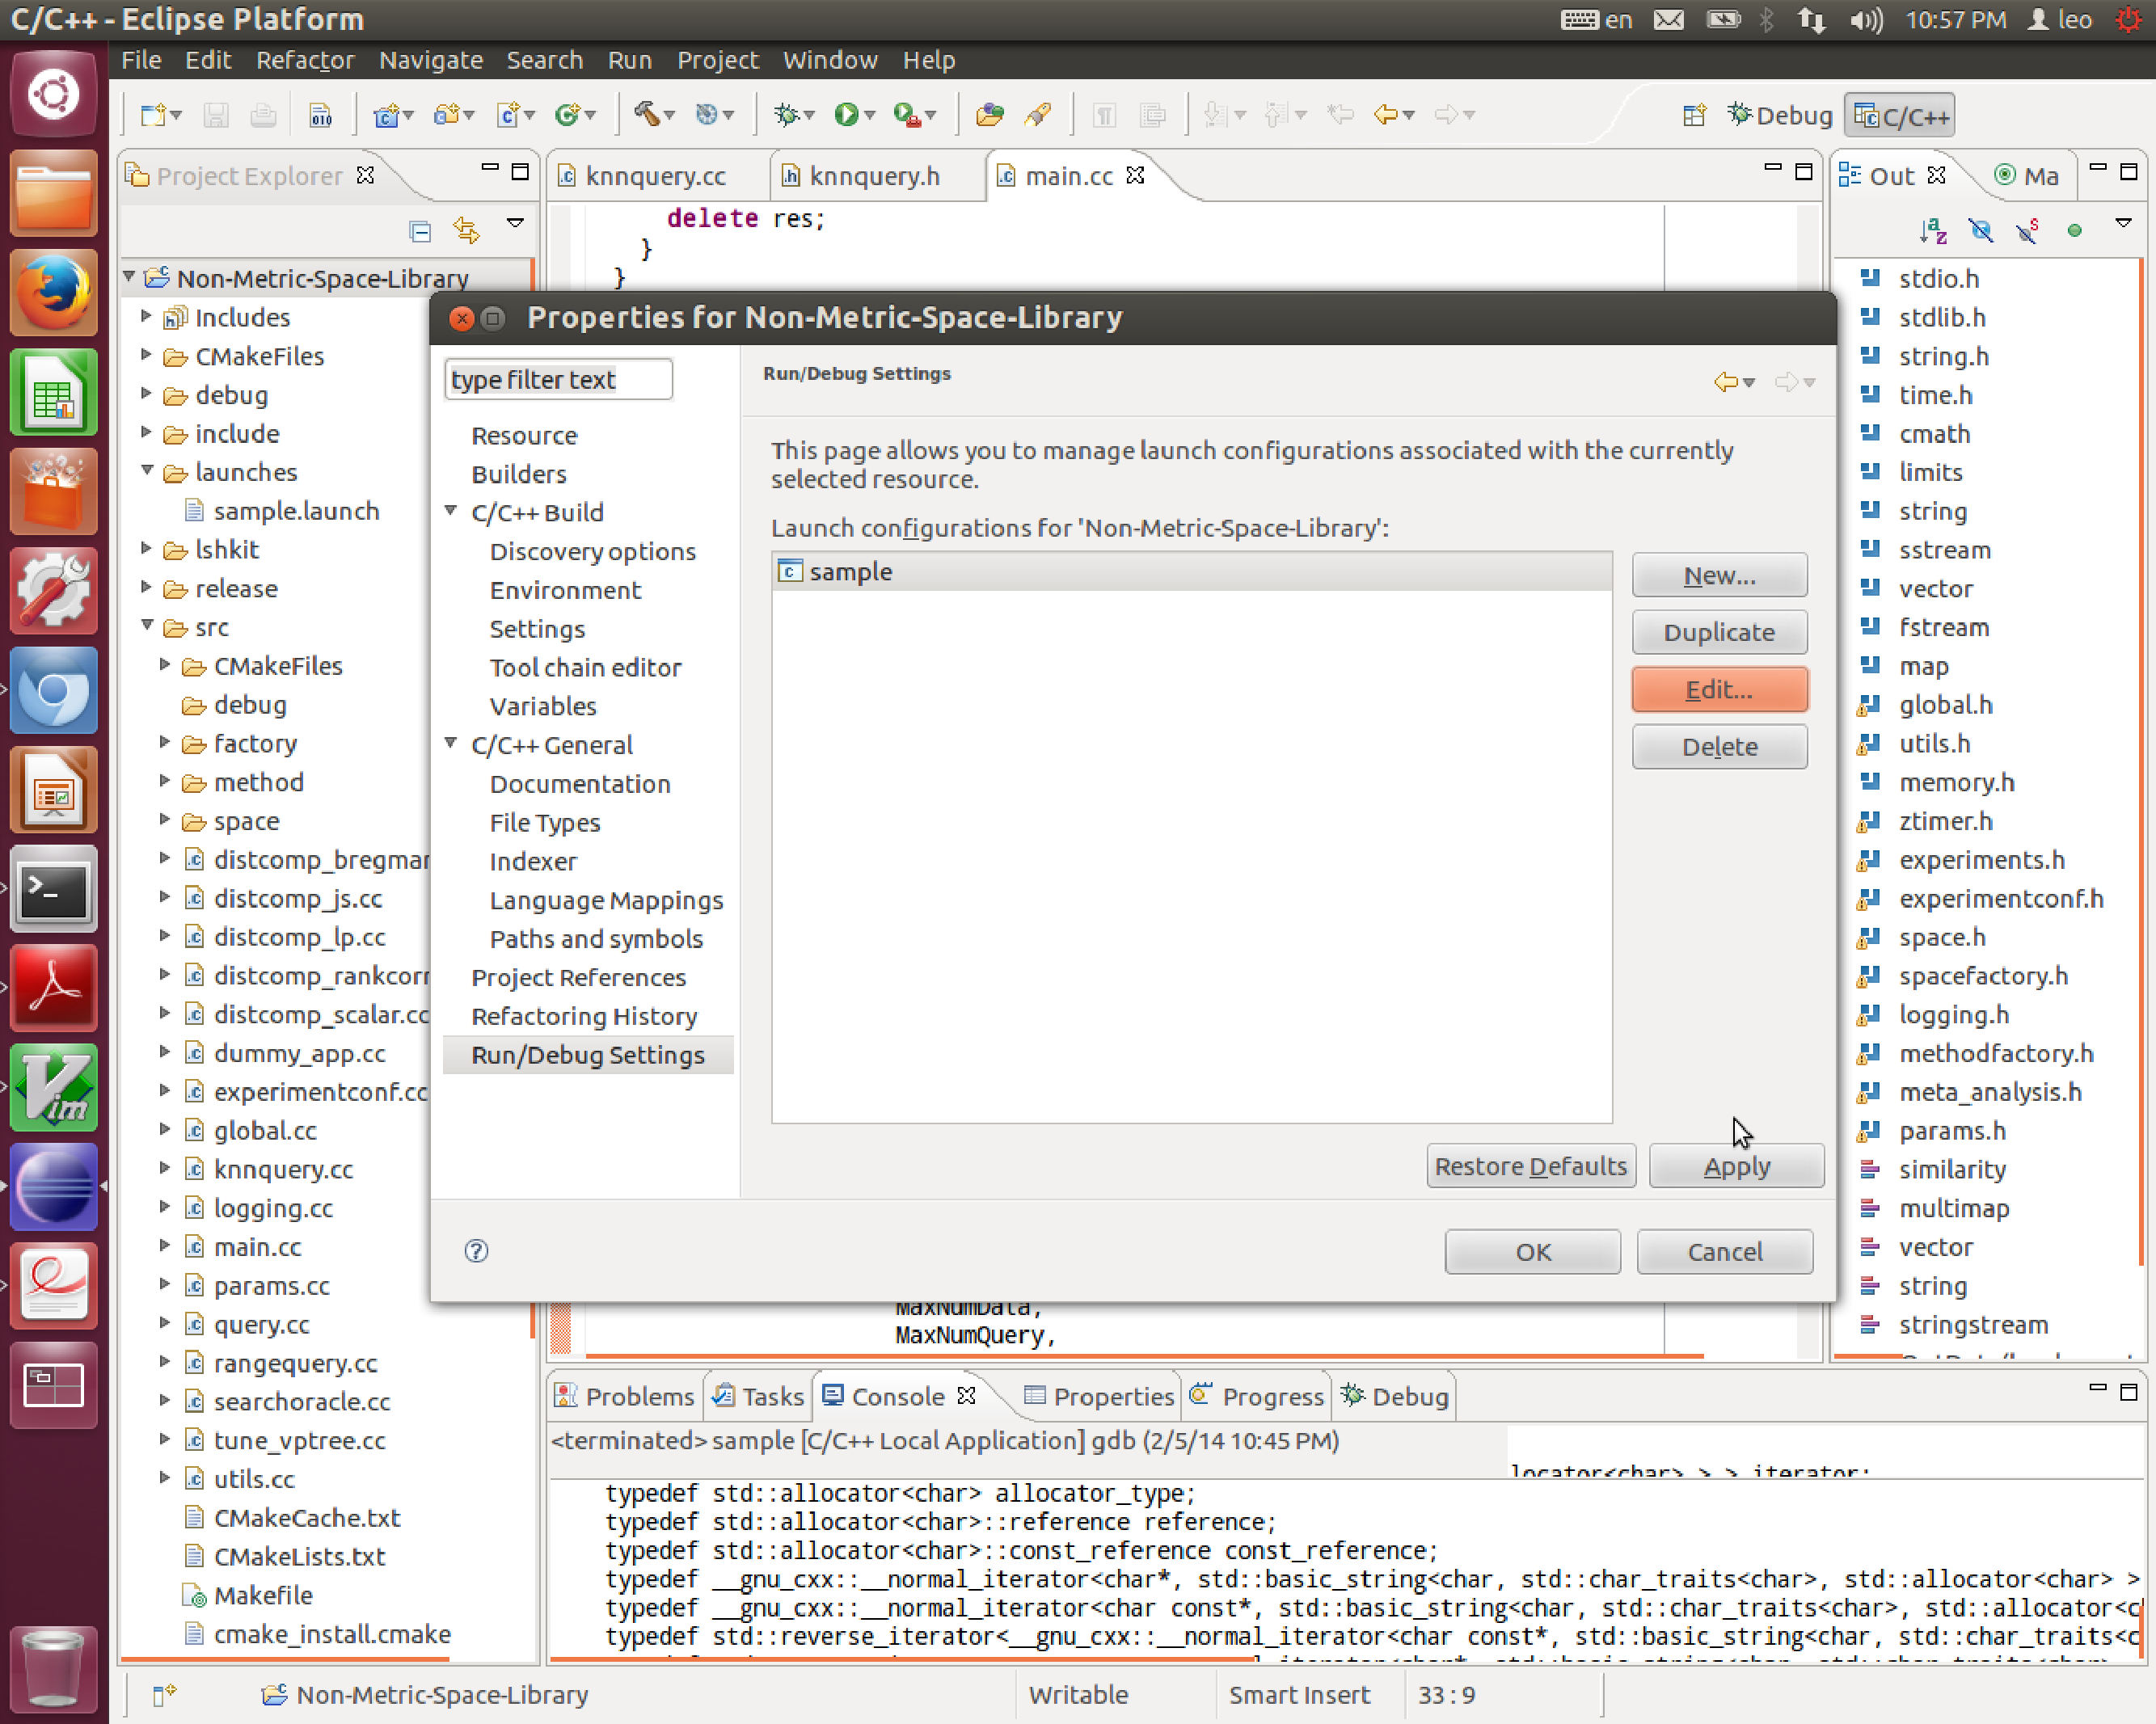
\includegraphics[width=0.9\textwidth]{figures/EclipseDebugConf.pdf}
\end{figure}

After building you can debug the project.
To do this, you need to create a debug configuration.
As an example, one configuration can be found in the 
project folder \ttt{launches}.
Right click on the item \ttt{sample.launch},
choose the option \ttt{Debug as} (in the drop-down menu),
and click on \ttt{sample} (in the pop-up menu).
Do not forget to edit command line arguments before you actually debug the application!

After switching to a debug perspective,
the Eclipse may stop the debugger in 
the file \ttt{dl-debug.c} as shown in Fig.~\ref{FigDebug}.
If this happened, simply, press the continue icon a couple of
times until the debugger enters the code belonging to the library.

Additional configurations can be created by right clicking
on the project name (left pane), selecting \ttt{Properties}
in the pop-up menu and clicking on \ttt{Run/Debug settings}. 
The respective screenshot is shown in Fig.~\ref{FigDebugConf}.


\begin{figure}
\centering
\caption{\label{FigDebug}Starting a debugger}
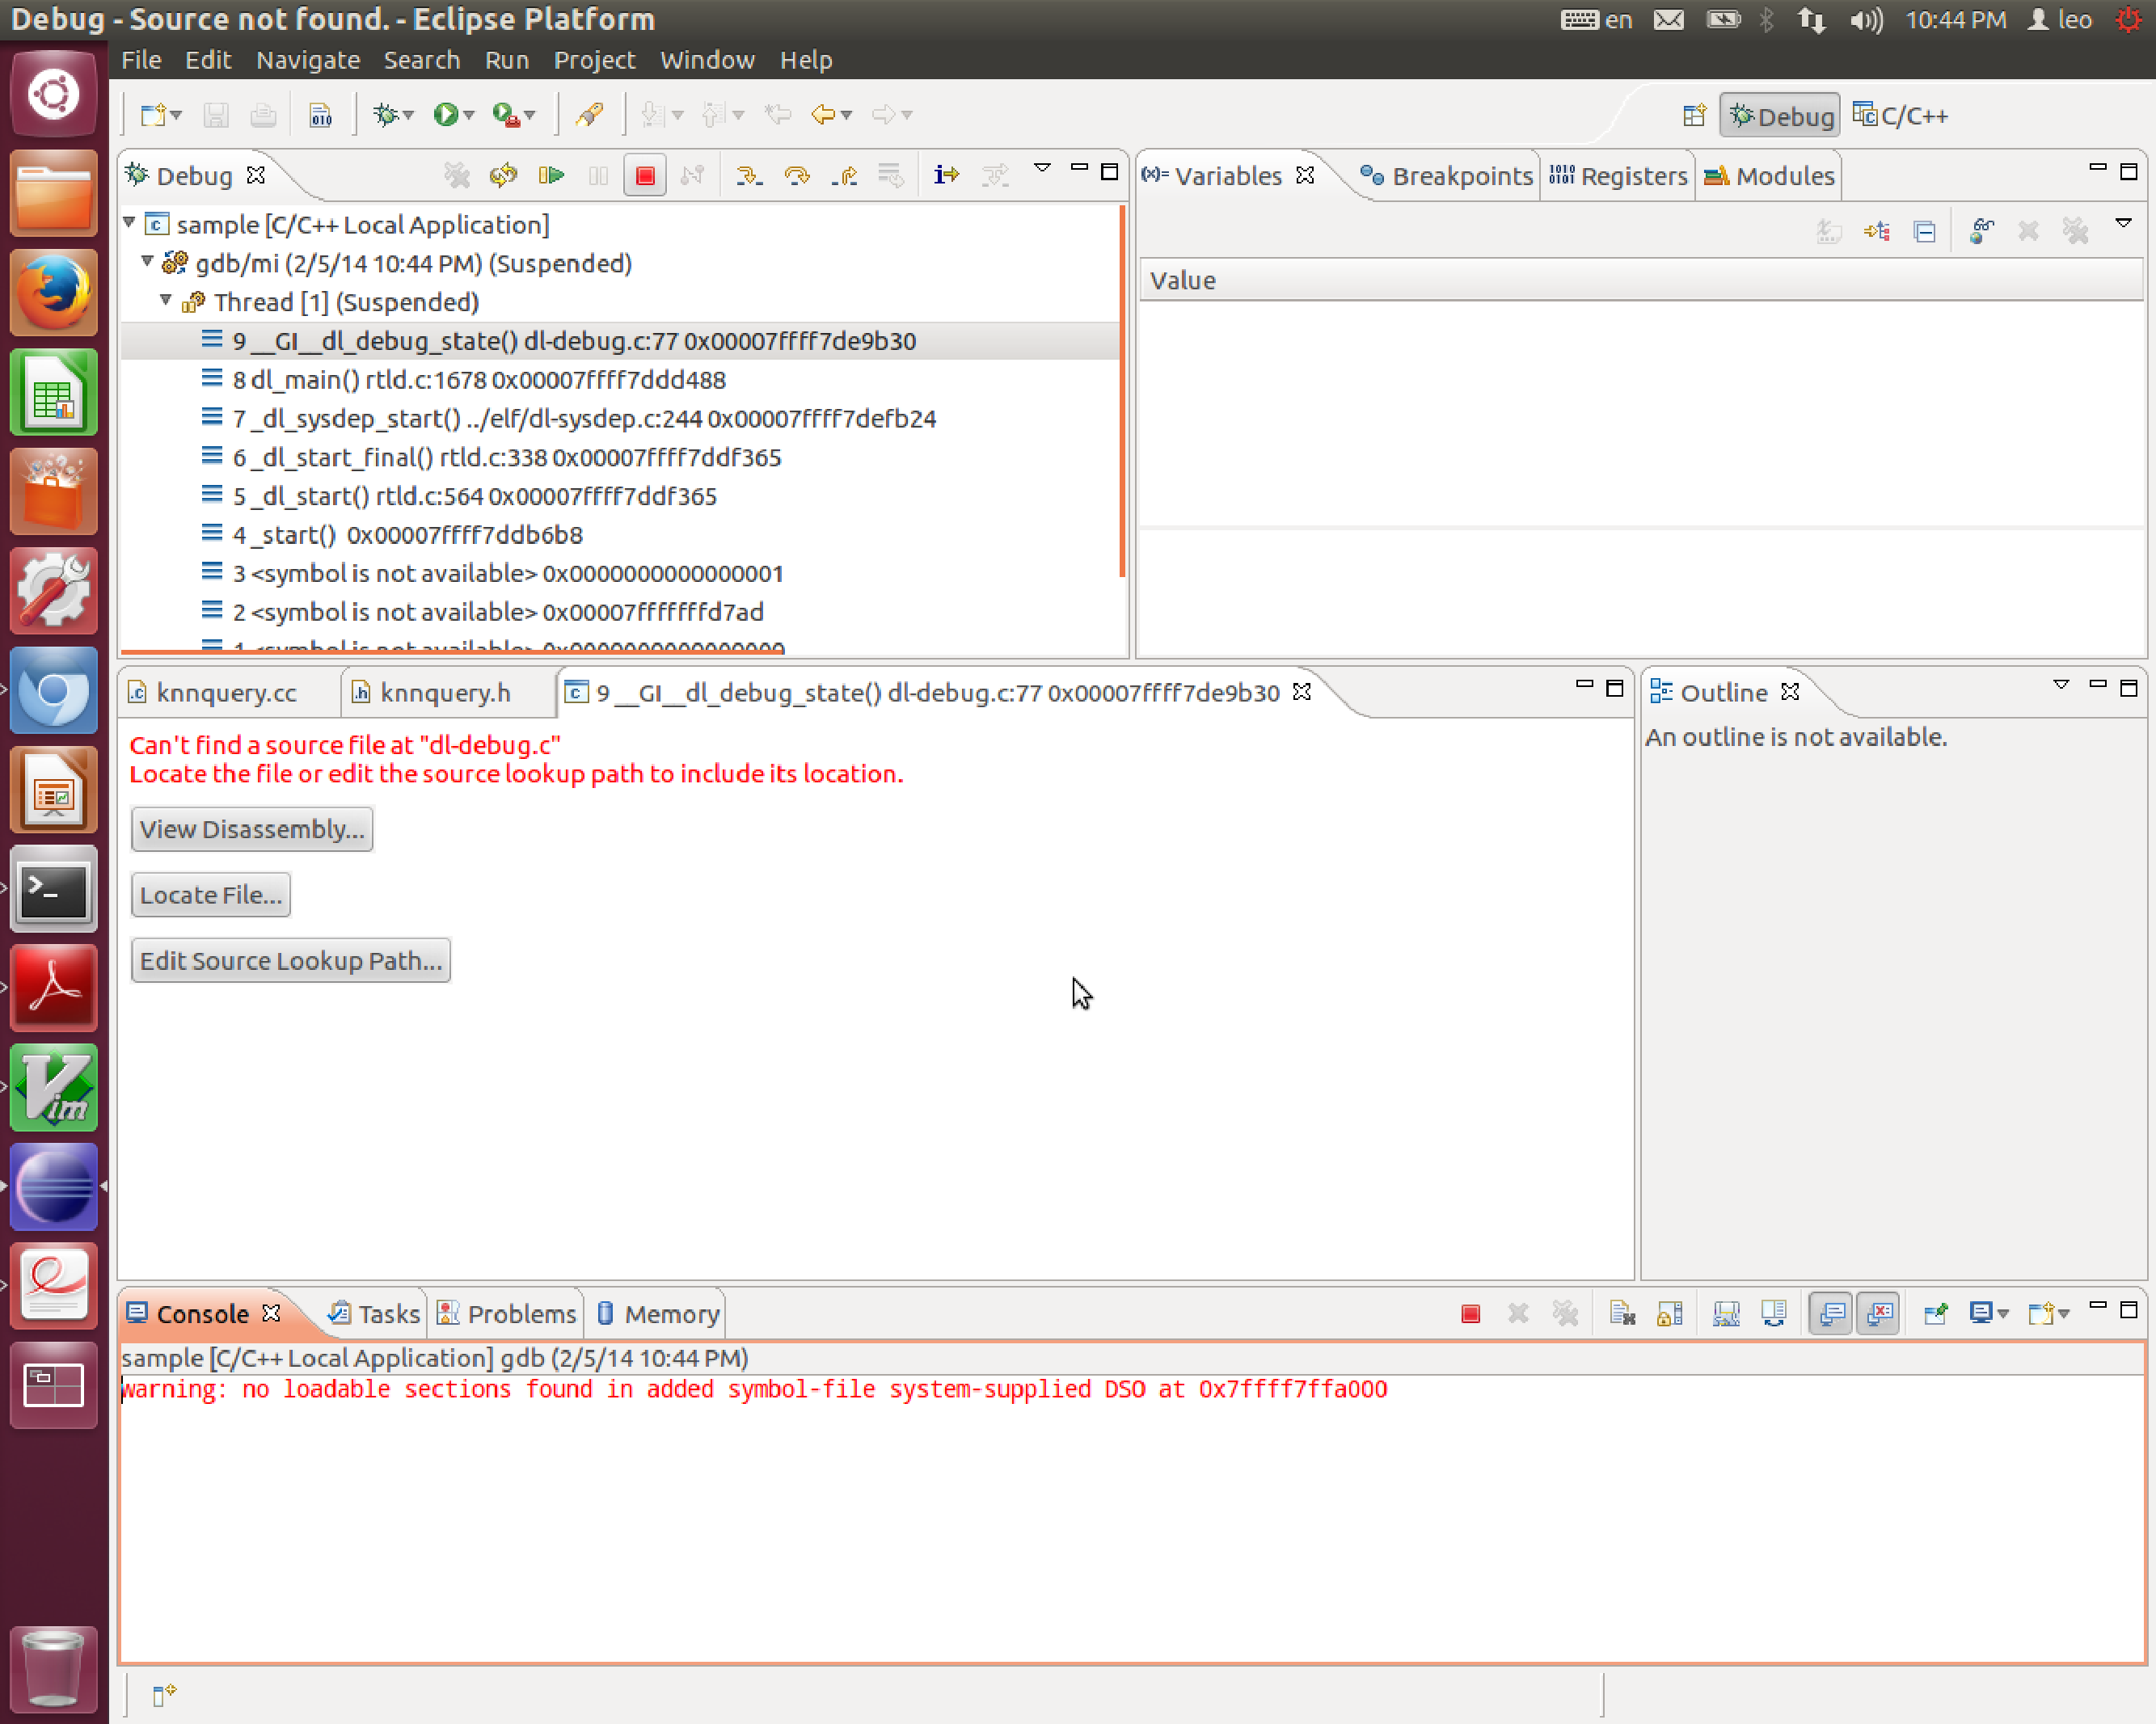
\includegraphics[width=0.9\textwidth]{figures/EclipseDebug.pdf}
\end{figure}


Note that this manual contains only a basic introduction to Eclipse.
If the user is new to Eclipse, we recommend reading
additional \href{http://www.eclipse.org/ide/}{documentation available online}.


\subsection{Building under Windows}\label{SectionBuildWindows}

\begin{figure}
\centering
\caption{\label{FigAVXSet}Enabling advanced SIMD Instructions in the Visual Studio}
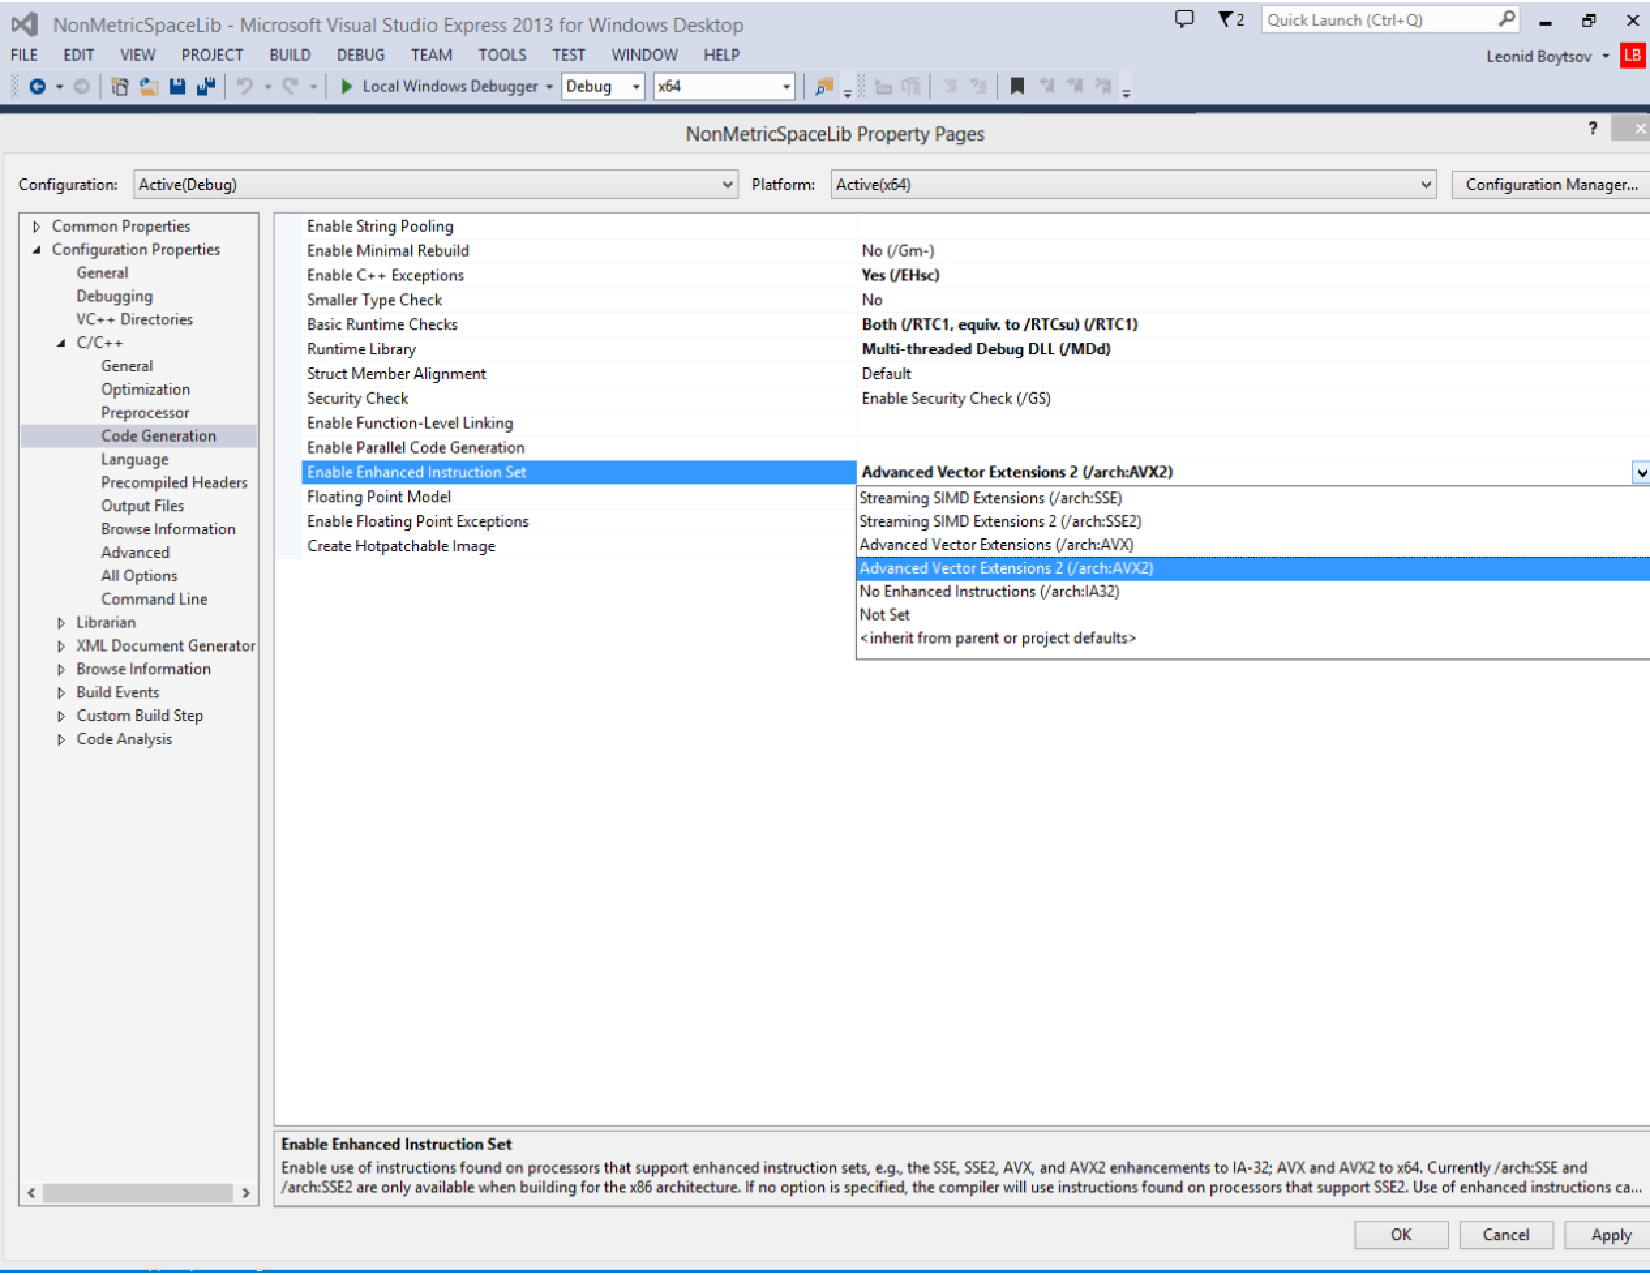
\includegraphics[width=0.9\textwidth]{figures/SettingAVXinVS2012.pdf}
\end{figure}

Download \href{https://www.visualstudio.com/en-us/downloads/download-visual-studio-vs.aspx}{Visual Studio 2015 Express for Desktop}. 
Download and install respective \href{http://sourceforge.net/projects/boost/files/boost-binaries/1.59.0/boost_1_59_0-msvc-14.0-64.exe/download}{Boost binaries}. Please, use the \textbf{default} installation directory on disk \ttt{c:}.
In the end of the section, we explain how to select a different location of the Boost files,
as well as to how downgrade the project to build it with Visual Studio 2013 (if this is really necessary). 

After downloading Visual Studio and installing Boost (version 59, 64-bit binaries, for MSVC-14), it is straightforward to build the project
using the provided \href{\replocfile similarity_search/NonMetricSpaceLib.sln}{Visual Studio 
solution file}.
The solution file references several (sub)-project (\ttt{*.vcxproj}) files,
which can be built either separately or all together.

The main sub-project is \ttt{NonMetricSpaceLib}, which is built before any other sub-projects. 
Sub-projects: 
\ttt{sample\_standalone\_app1},
\ttt{sample\_standalone\_app2} 
are examples of using the library in a standalone mode.
Unlike building under Linux, we provide no installation procedure yet.
In a nutshell, the installation consists in copying the library binary
as well as \href{\replocdir similarity_search/include}{the directory} with header files.

There are three possible configurations for the binaries: 
\ttt{Release}, \ttt{Debug}, and \ttt{RelWithDebInfo} (release with debug information). 
The corresponding output files are placed into the subdirectories:
\begin{verbatim}
  similarity_search\x64\Release,
  similarity_search\x64\Debug,
  similarity_search\x64\RelWithDebInfo.
\end{verbatim}

Unlike other compilers, there seems to be no way to detect the CPU type in the Visual Studio automatically.\footnote{It is not also possible to opt for using \href{http://en.wikipedia.org/wiki/SSE4}{only SSE4}.}
And, by default, only SSE2 is enabled (because it is supported by all 64-bit CPUs).
Therefore, if the user's CPU supports \href{https://en.wikipedia.org/wiki/Advanced_Vector_Extensions}{AVX extensions}, it is recommended to modify code generation settings as shown in the screenshot in Fig.~\ref{FigAVXSet}.
This should be done for \textbf{all} sub-projects and \textbf{all} binary configurations.
Note that you can set a property for all projects at once, if you select all the sub-projects, right-click, and then choose \ttt{Properties} 
in the pop-up menu.

\begin{figure}
\centering
\caption{\label{FigBoostSet}Specifying Location of Boost libraries}
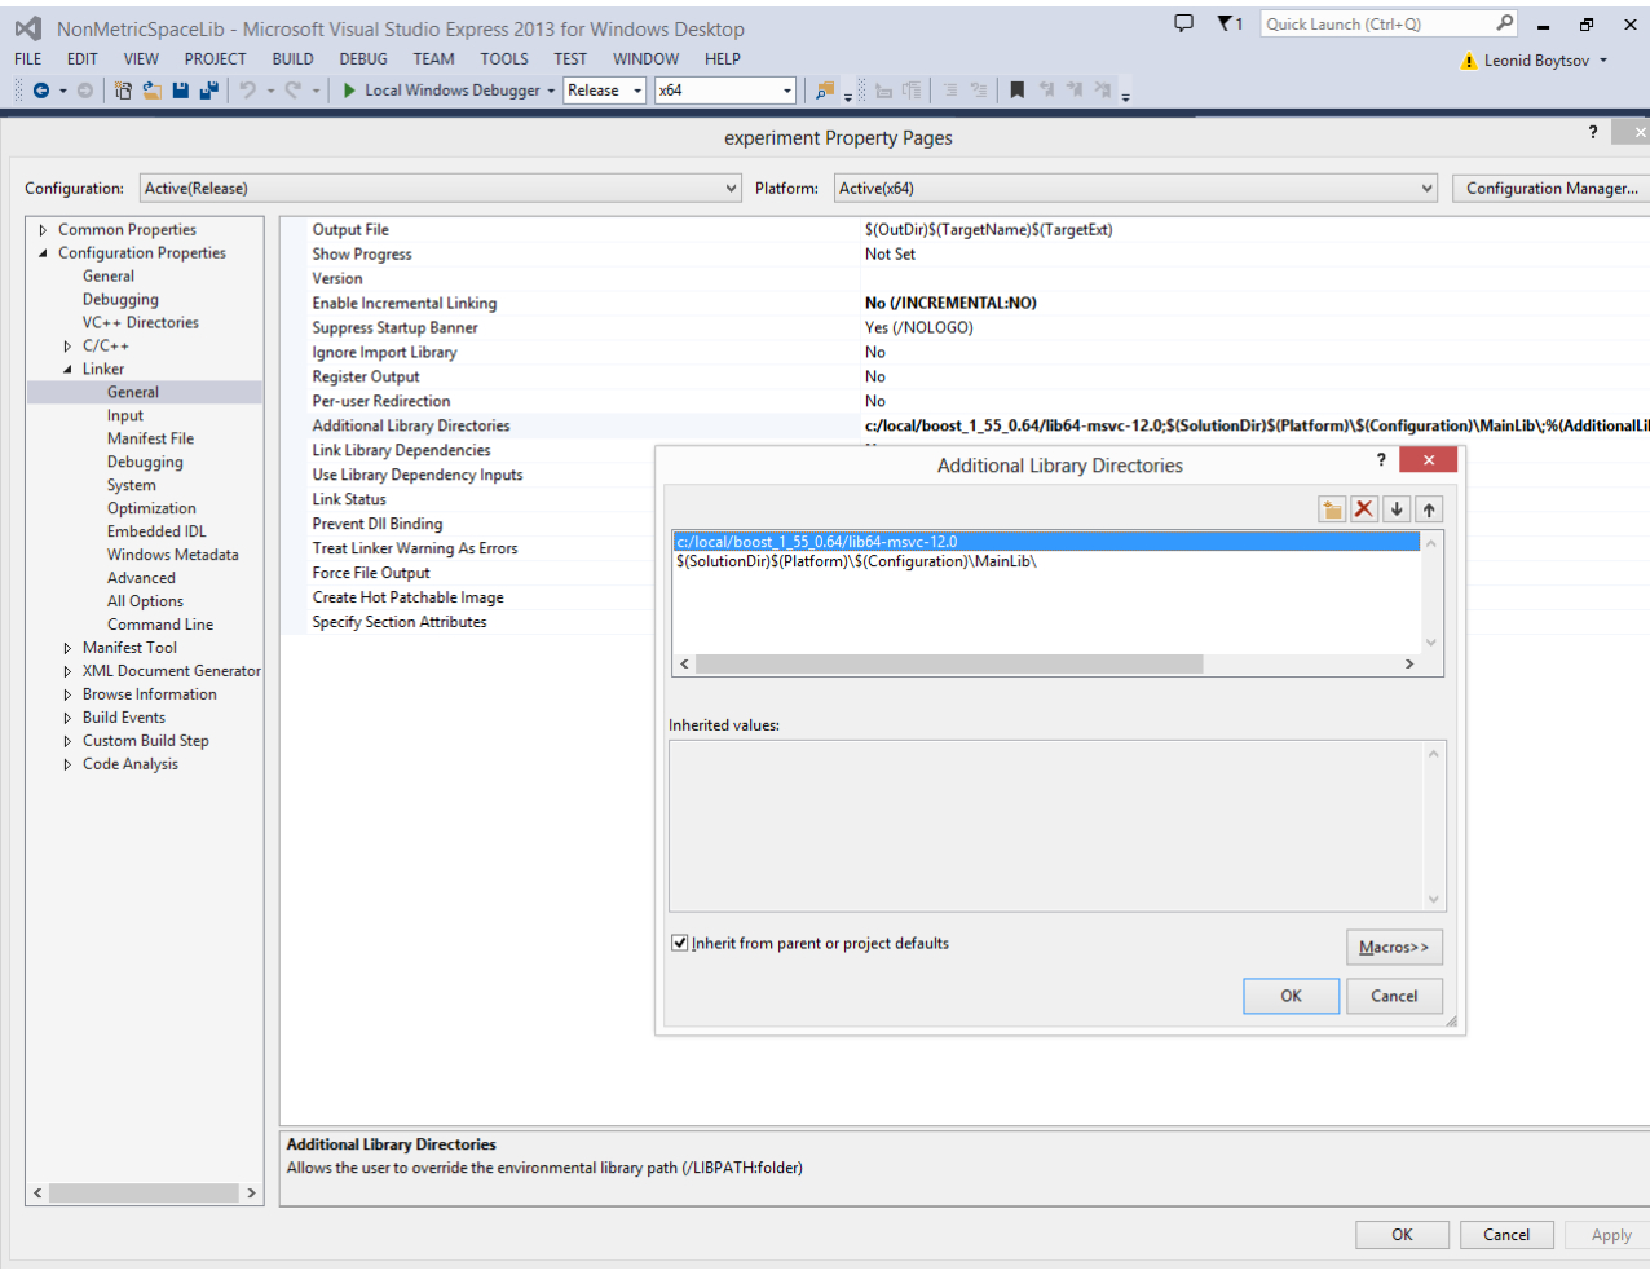
\includegraphics[width=0.9\textwidth]{figures/SettingBoostLocation.pdf}
\end{figure}

The core library, the semi unit test binary as well as examples of the standalone applications
can be built without installing Boost. 
However, Boost libraries are required for the binaries \ttt{experiment.exe}, \ttt{tune\_vptree.exe}, and \ttt{test\_integr.exe}.

We would re-iterate that one needs 64-bit Boost binaries compiled with the same version of the Visual Studio as the NMSLIB binaries.  
If you \href{http://sourceforge.net/projects/boost/files/boost-binaries/1.59.0/boost_1_59_0-msvc-14.0-64.exe/download}{download the installer for Boost 59} and install it to a default location, then you do not have to change project files.
Should you install Boost into a different folder, 
the location of Boost binaries and header file need to be specified in the 
project settings for all three build configurations (\ttt{Release}, \ttt{Debug}, \ttt{RelWithDebInfo}). An example of specifying the location of Boost libraries (binaries) is given in Fig.~\ref{FigBoostSet}.

In the unlikely case that the user has to use older Visual Studio 12, the project files are to be downgraded.
To do so, one have to manually edit every \ttt{*.vcxproj} file by replacing 
each occurrence of \ttt{<PlatformToolset>v140</PlatformToolset>} with \ttt{<PlatformToolset>v120</PlatformToolset>}.
Additionally, one has to download Boost binaries compatible with the older Visual studio and modify the project files
accordingly.
In particular, one may need to modify options \ttt{Additional Include Directories} and \ttt{Additional Library Directories}.

\subsection{Testing the Correctness of Implementations}
We have two main testing utilities \ttt{bunit} and \ttt{test\_integr} (\ttt{experiment.exe} and
\ttt{test\_integr.exe} on Windows).
Both utilities accept the single optional argument: the name of the log file.
If the log file is not specified, a lot of informational messages are printed to the screen.

The \ttt{bunit} verifies some basic functitionality akin to unit testing.
In particular, it checks that an optimized version of the, e.g., Eucledian, distance
returns results that are very similar to the results returned by unoptimized and simpler version.
The utility \ttt{bunit} is expected to always run without errors.

The utility \ttt{test\_integr} runs complete implementations of many methods
and checks if several effectiveness and efficiency characteristics
meet the expectations.
The expectations are encoded as an array of instances of the class \ttt{MethodTestCase}
(see \href{\replocdir /similarity_search/test/test_integr.cc#L65}{the code here}).
For example, we expect that the recall (see \S~\ref{SectionEffect})
fall in a certain pre-recorded range.
Because almost all our methods are randomized, there is a great deal of variance
in the observed performance characteristics. Thus, some tests
may fail infrequently, if e.g., the actual recall value is slightly lower or higher 
than an expected minimum  or maximum.
From an error message, it should be clear if the discrepancy is substantial, i.e.,
something went wrong, or not, i.e., we observe an unlikely outcome due to randomization.
The exact search method, however, should always have an almost perfect recall.

Variance is partly due to using low-dimensional test sets. In the future, we plan to change this.
For high-dimensional data sets, the outcomes are much more stable despite the randomized nature
of most implementations.
\subsection{Running Benchmarks}\label{SectionRunBenchmark}
There are no principal differences in benchmarking on Linux and Windows.
There is a \emph{single} benchmarking utility 
\ttt{experiment} (\ttt{experiment.exe} on Windows) that includes implementation of all methods.
It has multiple options, which specify, among others, 
a space, a data set, a type of search, a method to test, and method parameters.
These options and their use cases are described in the following subsections.
Note that unlike older versions it is not possible to test multiple methods in a single run.
However, it is possible to test the single method with different values of query-time parameters.

\subsubsection{Space and distance value type}

A distance function can return an integer (\ttt{int}), a single-precision (\ttt{float}),
or a double-precision (\ttt{double}) real value.
A type of the distance and its value is specified as follows:

\begin{verbatim}
  -s [ --spaceType ] arg       space type, e.g., l1, l2, lp:p=0.25
  --distType arg (=float)      distance value type: 
                               int, float, double
\end{verbatim}

A description of a space may contain parameters (parameters may not contain whitespaces).
In this case, there is colon after the space mnemonic name followed by a
comma-separated (not spaces) list of parameters in the format:
\ttt{<parameter name>=<parameter value>}.
Currently, this is used only for $L_p$ spaces. For instance,
 \ttt{lp:0.5} denotes the space $L_{0.5}$.
A detailed list of possible spaces and respective
distance functions is given in Table~\ref{TableSpaces} in \S~\ref{SectionSpaces}.

For real-valued distance functions, one can use either single- or double-precision
type. Single-precision is a recommended default.
One example of integer-valued distance function the Levenshtein distance.

\subsubsection{Input Data/Test Set}
There are two options that define the data to be indexed:
\begin{verbatim}
  -i [ --dataFile ] arg             input data file
  -D [ --maxNumData ] arg (=0)      if non-zero, only the first maxNumData 
                                    elements are used
\end{verbatim}
The input file can be indexed either completely, or partially.
In the latter case, the user can create the index using only
the first \ttt{--maxNumData} elements.

For testing, the user can use a separate query set.
It is, again, possible to limit the number of queries:
\begin{verbatim}
  -q [ --queryFile ] arg        query file
  -Q [ --maxNumQuery ] arg (=0) if non-zero, use maxNumQuery query 
                                elements(required in the case 
                                of bootstrapping)
\end{verbatim}
If a separate query set is not available, it can be simulated by bootstrapping.
To this, end the \ttt{--maxNumData} elements of the original data set
are randomly divided into testing and indexable sets.
The number of queries in this case is defined by the option \ttt{--maxNumQuery}.
A number of bootstrap iterations is specified through an option:
\begin{verbatim}
  -b [ --testSetQty ] arg (=0) # of sets created by bootstrapping; 
\end{verbatim}
Benchmarking can be carried out in either a single- or a multi-threaded
mode. The number of test threads are specified as follows:
\begin{verbatim}
 --threadTestQty arg (=1)   # of threads
\end{verbatim}

\subsubsection{Query Type} 
Our framework supports the \knn and the range search.
The user can request to run both types of queries:
\begin{verbatim}
  -k [ --knn ] arg         comma-separated values of k 
                           for the k-NN search
  -r [ --range ] arg       comma-separated radii for range search
\end{verbatim}
For example, by specifying the options 
\begin{verbatim}
--knn 1,10 --range 0.01,0.1,1
\end{verbatim}
the user requests to run queries of five different types: $1$-NN, $10$-NN,
as well three range queries with radii 0.01, 0.1, and 1.

\subsubsection{Method Specification}
Unlike older versions it is possible to test only a single method at a time.
To specify a method's name, use the following option:
\begin{verbatim}
  -m [ --method ] arg           method/index name
\end{verbatim}
A method can have a single set of index-time parameters, which is specified
via:
\begin{verbatim}
-c [ --createIndex ] arg        index-time method(s) parameters
\end{verbatim}
In addition to the set of index-time parameters,
the method can have multiple sets of query-time parameters, which are specified
using the following (possibly repeating) option:
\begin{verbatim}
-t [ --queryTimeParams ] arg    query-time method(s) parameters
\end{verbatim}
For each set of query-time parameters, i.e., for each occurrence of the option \ttt{--queryTimeParams}, 
the benchmarking utility \ttt{experiment},
carries out an evaluation using the specified set of queries and a query type (e.g., a 10-NN search with
queries from a specified file). 
If the user does not specify any query-time parameters, there is only one evaluation to be carried out.
This evaluation uses default query-time parameters.

Similar to parameters of the spaces, 
a set of method's parameters is a comma-separated list (no-spaces)
of parameter-value pairs in the format:
\ttt{<parameter name>=<parameter value>}.
For a detailed list of methods and their parameters, please, refer to \S~\ref{SectionMethods}.

Note that a few methods can save/restore (meta) indices. To save and load indices
one should use the following options:
\begin{verbatim}
  -L [ --loadIndex ] arg        a location to load the index from 
  -S [ --saveIndex ] arg        a location to save the index to
\end{verbatim}
When the user defines the location of the index using the option \ttt{--loadIndex}, 
the index-time parameters may be ignored. 
Specifically, if the specified index does not exist, the index is created from scratch.
Otherwise, the index is loaded from disk.
Also note that the benchmarking utility \emph{does not override an already existing index} (when the option \ttt{--saveIndex} is present).

If the tests are run the bootstrapping mode, i.e., when queries are randomly sampled (without replacement) from the
data set, several indices may need to be created. Specifically, for each split we create a separate index file.
The identifier of the split is indicated using a special suffix.
Also note that we need to memorize which data points in the split were used as queries. 
This information is saved in a gold standard cache file (see \S~\ref{SectionEfficiency}).
Thus, saving and loading of indices in the bootstrapping mode is possible only if 
gold standard caching is used.

\subsubsection{Saving and Processing Benchmark Results}
The benchmarking utility may produce output of three types:
\begin{itemize}
\item Benchmarking results (a human readable report and a tab-separated data file);
\item Log output (which can be redirected to a file);
\item Progress bars to indicate the progress in index creation for some methods (cannot be currently suppressed);
\end{itemize}

To save benchmarking results to a file, on needs to specify a parameter:
\begin{verbatim}
  -o [ --outFilePrefix ] arg  output file prefix
\end{verbatim}
As noted above, we create two files: a human-readable report (suffix \ttt{.rep}) and 
a tab-separated data file (suffix \ttt{.data}).
By default, the benchmarking utility creates files from scratch:
If a previously created report exists, it is erased. 
The following option can be used to append results to the previously created report:
\begin{verbatim}
  -a [ --appendToResFile ]    do not override information in results
\end{verbatim}
For information on processing and interpreting results see \S~\ref{SectionMeasurePerf}.
A description of the plotting utility is given in \S~\ref{SectionGenPlot}.

By default, all log messages are printed to the standard error stream.
However, they can also be redirected to a log-file:
\begin{verbatim}
  -l [ --logFile ] arg         log file
\end{verbatim}

\subsubsection{Efficiency of Testing}\label{SectionBenchEfficiency}
Except for  measuring methods' performance, 
the following are the most expensive operations: 
\begin{itemize}
\item computing ground truth answers (also
known as \emph{gold standard} data);
\item loading the data set; 
\item indexing. 
\end{itemize}
To make testing faster, the following methods can be used: 
\begin{itemize}
\item Caching of gold standard data;
\item Creating gold standard data using multiple threads; 
\item Reusing previously created indices (when loading and saving is supported by a method);
\item Carrying out multiple tests using different sets of query-time parameters. 
\end{itemize}

By default, we recompute gold standard data every time we run benchmarks, which may take long time.
However, it is possible to save gold standard data and re-use it later
by specifying an additional argument:
\begin{verbatim}
-g [ --cachePrefixGS ] arg  a prefix of gold standard cache files
\end{verbatim}
The benchmarks can be run in a multi-threaded mode by specifying a parameter:
\begin{verbatim}
--threadTestQty arg (=1)    # of threads during querying
\end{verbatim}
In this case, the gold standard data is also created in a multi-threaded mode (which can also be much faster).
Note that NMSLIB directly supports only an inter-query parallelism, i.e., multiple queries are executed in parallel,
rather than the intra-query parallelism, where a single query can be processed by multiple CPU cores.

Gold standard data is stored in two files. One is a textual meta file
that memorizes important input parameters such as the name of the data and/or query file,
the number of test queries, etc. 
For each query, the binary cache files contains ids of answers (as well as distances and 
class labels). 
When queries are created by random sampling from the main data set,
we memorize which objects belong to each query set.

When the gold standard data is reused later,
the benchmarking code verifies if input parameters match the content of the cache file. 
Thus, we can prevent an accidental use of gold standard data created for one data set
while testing with a different data set.

Another sanity check involves verifying that data points obtained via an approximate
search are not closer to the query than data points obtained by an exact search.
This check has turned out to be quite useful. 
It has helped detecting a problem in at least the following two cases:
\begin{itemize}
\item The user creates a gold standard cache. Then, the user modifies a distance function and runs the tests again;
\item Due to a bug, the search method reports distances to the query that are smaller than
the actual distances (computed using a distance function). This may occur, e.g., due to
a memory corruption.
\end{itemize}

When the benchmarking utility detects a situation when an approximate method
returns points closer than points returned by an exact method, the testing procedure is terminated
and the user sees a diagnostic message (see Table~\ref{TableFailGSCheck} for an example). 

\begin{table}
\scriptsize
\begin{verbatim}
... [INFO] >>>> Computing effectiveness metrics for small_world_rand
... [INFO] Ex: -2.097 id = 140154 -> Apr: -2.111 id = 140154 1 - ratio: -0.0202 diff: -0.0221
... [INFO] Ex: -1.974 id = 113850 -> Apr: -2.005 id = 113850 1 - ratio: -0.0202 diff: -0.0221
... [INFO] Ex: -1.883 id = 102001 -> Apr: -1.898 id = 102001 1 - ratio: -0.0202 diff: -0.0221
... [INFO] Ex: -1.6667 id = 58445 -> Apr: -1.6782 id = 58445 1 - ratio: -0.0202 diff: -0.0221
... [INFO] Ex: -1.6547 id = 76888 -> Apr: -1.6688 id = 76888 1 - ratio: -0.0202 diff: -0.0221
... [INFO] Ex: -1.5805 id = 47669 -> Apr: -1.5947 id = 47669 1 - ratio: -0.0202 diff: -0.0221
... [INFO] Ex: -1.5201 id = 65783 -> Apr: -1.4998 id = 14954 1 - ratio: -0.0202 diff: -0.0221
... [INFO] Ex: -1.4688 id = 14954 -> Apr: -1.3946 id = 25564 1 - ratio: -0.0202 diff: -0.0221
... [INFO] Ex: -1.454 id = 90204 -> Apr: -1.3785 id = 120613 1 - ratio: -0.0202 diff: -0.0221
... [INFO] Ex: -1.3804 id = 25564 -> Apr: -1.3190 id = 22051 1 - ratio: -0.0202 diff: -0.0221
... [INFO] Ex: -1.367 id = 120613 -> Apr: -1.205 id = 101722 1 - ratio: -0.0202 diff: -0.0221
... [INFO] Ex: -1.318 id = 71704 -> Apr: -1.1661 id = 136738 1 - ratio: -0.0202 diff: -0.0221
... [INFO] Ex: -1.3103 id = 22051 -> Apr: -1.1039 id = 52950 1 - ratio: -0.0202 diff: -0.0221
... [INFO] Ex: -1.191 id = 101722 -> Apr: -1.0926 id = 16190 1 - ratio: -0.0202 diff: -0.0221
... [INFO] Ex: -1.157 id = 136738 -> Apr: -1.0348 id = 13878 1 - ratio: -0.0202 diff: -0.0221
... [FATAL] bug: the approximate query should not return objects that are closer to the query 
                 than object returned by (exact) sequential searching! 
                 Approx: -1.09269 id = 16190 Exact: -1.09247 id = 52950
\end{verbatim}
\caption{\label{TableFailGSCheck} A diagnostic message indicating that
there is some mismatch in the current experimental setup and the setup used to create
the gold standard cache file.}
\end{table}

To compute recall, it is enough to memorize only query answers.
For example, in the case of a 10-NN search, it is enough to memorize only 10 data points closest 
to the query as well as respective distances (to the query).
However, this is not sufficient for computation of  a rank approximation metric (see \S~\ref{SectionEffect}).
To control the accuracy of computation, we permit the user to change the number of entries memorized.
This number is defined by the parameter:
\begin{verbatim}
--maxCacheGSRelativeQty arg (=10)   a maximum number of gold 
                                    standard entries
\end{verbatim}
Note that this parameter is a coefficient: the actual number of entries is defined relative to
the result set size. For example, if a range search returns 30 entries and the value of 
\ttt{--maxCacheGSRelativeQty} is 10, then $30 \times 10=300$ entries are saved in the gold standard
cache file.

\subsection{Measuring Performance and Interpreting Results}\label{SectionMeasurePerf}
\subsubsection{Efficiency.} We measure several efficiency metrics: query runtime, the number of distance computations,
the amount of memory used by the index \emph{and} the data, and the time to create the index.
We also measure the improvement in runtime (improvement in efficiency) 
with respect to a sequential search (i.e., brute-force) approach
as well as an improvement in the number of distance computations. 
If the user runs benchmarks in a multi-threaded mode (by specifying the option \ttt{--threadTestQty}),
we compare against the multi-threaded version of the brute-force search as well.

A good method should
carry out fewer distance computations and be faster than the brute-force search,
which compares \emph{all the objects} directly with the query. 
However, great reduction in the number of distance computations 
does not always entail good improvement in efficiency:
while we do not spend CPU time on computing directly,
we may be spending CPU time on, e.g., computing the value of the distance 
in the projected space (as
in the case of projection-based methods, see \S~\ref{SectionProjMethod}).

Note that the improvement in efficiency is adjusted for the number of threads.
Therefore, it does not increase as more threads are added: in contrast,
it typically decreases as there is more competition for computing resources (e.g., memory)
in a multi-threaded mode.

The amount of memory consumed by a search method is measured indirectly: 
We record the overall memory usage of a benchmarking process before and after creation of the index. Then, we add the amount of memory used by the data.
On Linux,  we query a special file \ttt{/dev/<process id>/status},
which might not work for all Linux distributives.
Under Windows, we retrieve the working set size using the function
\ttt{GetProcessMemoryInfo}.
Note that we do not have  a truly portable code to measure memory consumption of a process.

\subsubsection{Effectiveness}
\label{SectionEffect}

In the following description, we assume that a method returns 
a set of points/objects $\{o_i\}$.
The value of $\pos(o_i)$ represents a positional distance from $o_i$ to the query, 
i.e., the number of database objects closer to the query than $o_i$ plus one.
Among objects with identical distances to the query, 
the object with the smallest index is considered to be the closest.
Note that $\pos(o_i) \ge i$.

Several effectiveness metrics are computed by the benchmarking utility:
\begin{itemize}
\item  A \emph{number of points closer} to the query than the nearest returned point.
This metric is equal $\pos(o_1)$ minus one. If $o_1$ is always the true nearest object,
its positional distance is one and, thus, the \emph{number of points closer} is always equal to zero.
\item A \emph{relative position} error for point $o_i$ is equal to $\pos(o_i)/i$,
an aggregate value is obtained by computing the geometric mean over all returned $o_i$;
\item \emph{Recall},  which is is equal to the fraction of all correct answers retrieved.
\item \emph{Classification accuracy}, which is equal to the fraction of labels correctly
predicted by a \knn based classification procedure.
\end{itemize}

The first two metrics represent a so-called rank (approximation) error.
The closer the returned objects are to the query object, 
the better is the quality of the search response and the lower is the rank 
approximation error.

\begin{wraptable}{R}{0.52\textwidth}
\caption{An example of a human-readable report 
\label{TableHRep}}
\begin{verbatim}
===================================
vptree: triangle inequality
alphaLeft=2.0,alphaRight=2.0
===================================
# of points: 9900
# of queries: 100
------------------------------------
Recall:         0.954 -> [0.95 0.96]
ClassAccuracy:  0     -> [0 0]
RelPosError:    1.05  -> [1.05 1.06]
NumCloser:      0.11  -> [0.09 0.12]
------------------------------------
QueryTime:      0.2   -> [0.19 0.21]
DistComp:       2991  -> [2827 3155]
------------------------------------
ImprEfficiency: 2.37  -> [2.32 2.42]
ImprDistComp:   3.32  -> [3.32 3.39]
------------------------------------
Memory Usage:   5.8 MB
------------------------------------
\end{verbatim}
\textbf{Note:} \emph{confidence intervals} are in brackets
%\vspace{-4em}
\end{wraptable}


Recall is a classic metric. 
It was argued, however, 
that recall does not account for positional information of returned objects
and is, therefore, inferior to rank approximation error metrics \cite{Amato_et_al:2003,Cayton2008}.
Consider the case of 10-NN search and imagine that there are two methods
that, on average, find only half of true 10-NN objects.
Also, assume that the first method always finds neighbors from one to five,
but misses neighbors from six to ten.
The second method always finds neighbors from six to ten, but misses the first five ones.
Clearly, the second method produces substantially inferior results, but it has the same recall as the first one.

If we specify ground-truth object classes (see \S~\ref{SectionDatasets} 
for the description of data set formats), 
it is possible to compute an accuracy of a \knn based classification procedure.
The label of an element is selected as the most frequent class label among $k$ closest objects
returned by the method (in the case of ties the class label with the smallest id is chosen).

If we had ground-truth queries and relevance judgements from human assessors,
we could in principle compute other realistic effectiveness metrics 
such as the mean average precision,
or the normalized discounted cumulative gain.
This remains for the future work.

Note that it is pointless to compute the mean average precision
when human judgments are not available, \href{http://searchivarius.org/blog/when-average-precision-equal-recall}{as the mean average precision
is identical to the recall in this case}.

\subsection{Interpreting and Processing Benchmark Results}
If the user specifies the option \ttt{--outFilePrefix},
the benchmarking results are stored to the file system.
A prefix of result files is defined by the parameter \ttt{--outFilePrefix}
while the suffix is defined by a type of the search procedure (the \knn or the range search)
as well as by search parameters (e.g., the range search radius).
For each type of search, two files are generated:
a report in a human-readable format,
and a tab-separated data file intended for automatic processing.
The data file contains only the average values,
which can be used to, e.g., produce efficiency-effectiveness plots
as described in \S~\ref{SectionGenPlot}.

\todonoteinline{Revise computation of confidence intervals}
An example of human readable report (\emph{confidence intervals} are in square brackets)
is given in Table~\ref{TableHRep}.
In addition to averages, the human-readable report provides 95\% confidence intervals.
In the case of bootstrapping, statistics collected for several splits of the data set are aggregated.
For the retrieval time and the number of distance computations,
this is done via a classic fixed-effect model adopted in meta analysis \cite{Hedges_and_Vevea:1998}.
When dealing with other performance metrics, 
we employ a simplistic approach of averaging split-specific values
and computing the sample variance over spit-specific averages.\footnote{The distribution
of many metric values is not normal. There are approaches to resolve this issue (e.g., apply a transformation),
but an additional investigation is needed to understand which approaches work best.}
Note for all metrics, except relative position error, an average is computed using an arithmetic mean.
For the relative error, however, we use the geometric mean  \cite{king:1986}.


\subsection{Plotting results}\label{SectionGenPlot}
We provide the Python script to generate nice performance graphs 
from tab-separated data file produced by the 
benchmarking utility \ttt{experiment}. 
The plotting script is \href{\replocfile sample_scripts/genplot_configurable.py}{genplot\_configurable.py}.
In addition to Python, it requires Latex and PGF. 
This script is supposed to run only on Linux.

Consider the following example of using \ttt{genplot\_configurable.py}:
\begin{verbatim}
../sample_scripts/genplot_configurable.py  \
           -n MethodName \
           -i result_K\=1.dat -o plot_1nn \
           -x 1~norm~Recall \
           -y 1~log~ImprEfficiency \
           -a  axis_desc.txt \
           -m  meth_desc.txt \
           -l "2~(0.96,-.2)" \
           -t "ImprEfficiency  vs Recall" \
           --xmin 0.01 --xmax 1.2 --ymin -2 --ymax 10
\end{verbatim}
Here the goal is to process the tab-separated data file \ttt{result\_K=1.dat},
which was generated by 1-NN search, and save the plot to the file \ttt{plot\_1nn.pdf}.
Note that one should not explicitly specify the extension of the output file (as
\ttt{.pdf} is always implied). Also note that, in addition to the PDF-file,
the script generates the source Latex file. 
The source Latex file can be post-edited and/or embedded directly into a Latex source 
(see \href{http://ftp.fau.de/ctan/graphics/pgf/base/doc/pgfmanual.pdf}{PGF documentation for details}).
This can be useful for scientific publishing.


The parameter \ttt{-n} specifies the name of the field that stores method/indices mnemonic names.
In the case of the benchmarking utility \ttt{experiment} this field is named \ttt{MethodName}.
Parameters \ttt{-x} and \ttt{-y} define  X and Y axis, i.e.,
which metrics are associated with each axis and what is the display format.
Parameter values have the same format.
Each parameter has three tilda-separated values. The first should
be zero or one.
Specify zero not to print the axis label.
The second value is either \ttt{norm} or \ttt{log}, 
which stands for a normal or logarithmic scale, respectively.
The last value defines a metric that we want to visualize:
The metric should be a field name, i.e.,
it is one of the names that appear in the header row of the output data file.
The title of the plot is defind by \ttt{-t} (specify \ttt{-t ""} if you do not want
to print the title).

For each metric, one has to specify the display name. To this end, the user supplies
an axis description file (option \ttt{-a}). This is a two-column tab-separated file.
The first column is a name of the metric used in the data file (in our example it is \ttt{result\_K=1.dat}).
The second column is a display name. Here is an example of the axis description file (tabs are not shown):
\begin{verbatim}
Recall        recall 
QueryTime     time (ms)
\end{verbatim}

Similarly, the user has to specify a method description file (option \ttt{-m}).
It is a three-column tab-separated file. The first column is the name of the method
used in the data file \ttt{result\_K=1.data} (\emph{exactly} as it is specified there).
The second column is the method display name (it can have Latex-parsable expressions). 
The third column, defines the style of the plot (e.g., line thickness and a line mark). 
This should be a comma-separated lists of PGF-specifiers 
(see \href{http://ftp.fau.de/ctan/graphics/pgf/base/doc/pgfmanual.pdf}{PGF documentation for details}).
Here is an example of the method description file (tabs again are not shown):
\begin{verbatim}
"bbtree"	bbtree	mark=triangle*
"vptree"	vptree	mark=star,blue,/tikz/densely dashed,mark size=1.5pt
\end{verbatim}

The parameter \ttt{-l} defines a plot legend.
It is either a string \ttt{none} (to hide the legend) 
or  it contains two tilda-separated values.
The first value gives the number of columns in the legend, while the second value
defines a position of the legend. The position can be either 
absolute or relative.
An absolute position is defined by a pair of coordinates (in round brackets).
A relative position is defined by one of the following descriptors 
(quotes are for clarity only): ``north west'', ``north east'', ``south west'', ``south east''.
If the relative position is specified, the legend is printed inside the main
plotting area, e.g.:
\begin{verbatim}
../sample_scripts/genplot.py  \
           -n MethodName \
           -i result_K\=1.dat -o plot_1nn \
           -x 1~norm~Recall \
           -y 1~log~ImprEfficiency \
           -a  axis_desc.txt \
           -m  meth_desc.txt \
           -l "2~north west" \
           -t "ImprEfficiency  vs Recall"
\end{verbatim}

Finally, note that the user can specify the bounding rectangle for the plot
via the options \ttt{--xmin}, \ttt{--xmax}, \ttt{--ymin}, and \ttt{--ymax}.

\section{Spaces}\label{SectionSpaces}
Currently we provide implementations mostly for vector spaces.
Vector-space input files can come in either regular, i.e., dense,
or sparse variant (see \S~\ref{SectionDatasets}). 
A detailed list of spaces, their parameters, 
and performance characteristics is given in Table~\ref{TableSpaces}.

The mnemonic name of the space is passed to the benchmarking utility (see \S~\ref{SectionRunBenchmark}).
There can be more than one version of a distance function,
which have different space-performance trade-off.
In particular, for distances that require computation of logarithms 
we can achieve an order of magnitude improvement (e.g., for the GNU C++
and Clang) by pre-computing
logarithms at index time. This comes at a price of extra storage. 
In the case of Jensen-Shannon distance functions, we can pre-compute some 
of the logarithms and accurately approximate those we cannot pre-compute.
The details are explained in \S~\ref{SectionLP}-\ref{SectionBregman}.

Straightforward slow implementations of the distance functions may have the substring \ttt{slow}
in their names, while faster versions contain the substring \ttt{fast}.
Fast functions that involve approximate computations contain additionally the substring \ttt{approx}.
For non-symmetric distance function, a space may have two variants: one variant is for left
queries (the data object is the first, i.e., left, argument of the distance function 
while the query object
is the second argument) 
and another is for right queries (the data object is the second argument and the query object is the first argument).
In the latter case the name of the space ends on \ttt{rq}.
Separating spaces by query types, might not be the best approach.
Yet, it seems to be unavoidable, because, in many cases,
we need separate indices to support left and right queries \cite{Cayton2008}.
If you know a better approach, feel free, to tell us.

\subsection{Details of Distance Efficiency Evaluation}\label{SectionDistEvalDetails}
Distance computation efficiency was evaluated on a Core i7 laptop (3.4 Ghz peak frequency)
in a single-threaded mode (by the utility \href{\replocfile similarity_search/test/bench_distfunc.cc}{bench\_distfunc}).
It is measured in millions of computations per second for single-precision
floating pointer numbers (double precision computations are, of course, more costly). 
The code was compiled using the GNU compiler. 
All data sets were small enough to fit in a CPU cache, which may have resulted in slightly more optimistic
performance numbers for cheap distances such as $L_2$.

Somewhat higher efficiency numbers can be obtained by using the Intel compiler
or the Visual Studio (Clang seems to be equally efficient to the GNU compiler).
In fact, performance is much better for distances relying on ``heavy'' math functions:
slow versions of KL- and Jensen-Shannon divergences and Jensen-Shannon metrics, 
as well as for $L_p$ spaces,
where $p \not\in\{1,2,\infty\}$.

In the efficiency test, all dense vectors have 128 elements.
For all dense-vector distances except the Jensen-Shannon divergence,
their elements were generated randomly and uniformly.
For the Jensen-Shannon divergence, we first generate elements randomly,
and next we randomly select elements that are set to zero (approximately half of all elements). 
Additionally, for KL-divergences and the JS-divergence,
we normalize vector elements so that they correspond a true discrete probability distribution. 

Sparse space distances were tested using sparse vectors from two sample files in the
\href{\replocfile sample_data}{sample\_data} directory.
Sparse vectors in 
\href{\replocfile sample_data/sparse_5K.txt}{the first} 
and
\href{\replocfile sample_data/sparse_wiki_5K.txt}{the second file} on average contain
about 100 and 600 non-zero elements, respectively.

String distances were tested using \href{\replocfile sample_data/dna32_4_5K.txt}{DNA sequences} sampled from a human genome.\footnote{\url{http://hgdownload.cse.ucsc.edu/goldenPath/hg38/bigZips/}}
The length of each string was sampled from a normal distribution $\mathcal{N}(32,4)$. 

The Signature Quadratic Form Distance (SQFD) \cite{Beecks:2010,Beecks:2013} was tested 
using signatures extracted from LSVRC-2014 data set~\cite{ILSVRCarxiv14}, 
which contains 1.2 million high resolution images.
We implemented \href{\replocfile data/data\_conv/sqfd}{our own code} to extract signatures following the method of Beecks~\cite{Beecks:2013}.
For each image, we selected $10^4$ pixels randomly and
mapped them into 7-dimensional feature space:
three color, two position, and two texture dimensions.
The features were clustered by the standard $k$-means algorithm with 20 clusters.
Then, each cluster was represented by an 8-dimensional vector, which included
a 7-dimensional centroid and a cluster weight (the number of cluster points divided
by $10^4$).

\begin{table}
\caption{Description of implemented spaces\label{TableSpaces}}
%\centering
\hspace{-0.6in}\begin{tabular}{l@{\hspace{2mm}}l@{\hspace{2mm}}l}
\toprule
\textbf{Space}& \textbf{Mnemonic Name \& Formula}   & \textbf{Efficiency} \\
              &                           & (million op/sec) \\
\toprule
\multicolumn{3}{c}{\textbf{Metric Spaces}}  \\
\toprule
Hamming &  \ttt{bit\_hamming}                      &  240 \\
                 &  $\sum_{i=1}^n |x_i-y_i|$                         &  \\
\cmidrule(l){1-3} 
$L_1$     &  \ttt{l1}, \ttt{l1\_sparse}              &                   35, 1.6 \\
                 &  $\sum_{i=1}^n |x_i-y_i|$                         &  \\
\cmidrule(l){1-3} 
$L_2$     &  \ttt{l2}, \ttt{l2\_sparse}              &                  30, 1.6  \\
                 & $\sqrt{\sum_{i=1}^n |x_i-y_i|^2}$                 &   \\
\cmidrule(l){1-3} 
$L_{\infty}$ &  \ttt{linf}, \ttt{linf\_sparse}      &   34 , 1.6  \\
                    & $\max_{i=1}^n |x_i-y_i|$           & \\
\cmidrule(l){1-3} 
$L_p$ (generic $p \ge 1$)& \ttt{lp:p=\ldots}, \ttt{lp\_sparse:p=\ldots}  &  0.1-3, 0.1-1.2  \\
                                & $\left(\sum_{i=1}^n |x_i-y_i|^p\right)^{1/p}$  & \\
\cmidrule(l){1-3} 
Angular distance & \ttt{angulardist}, \ttt{angulardist\_sparse}, \ttt{angulardist\_sparse\_fast} & { 13, 1.4, 3.5 } \\
                        & $\arccos\left(\frac{\sum_{i=1}^n x_i y_i}{\sqrt{\sum_{i=1}^n x_i^2}\sqrt{\sum_{i=1}^n y_i^2 }}\right)$   & \\
\cmidrule(l){1-3} 
Jensen-Shan. metr. &\ttt{jsmetrslow, jsmetrfast, jsmetrfastapprox} &  0.3, 1.9, 4.8  \\
                          & $\sqrt{\frac{1}{2}\sum_{i=1}^n \left[x_i \log x_i + y_i \log y_i  - (x_i+y_i)\log \frac{x_i +y_i}{2}\right]}$  & \vspace{1em} \\
\cmidrule(l){1-3} 
Levenshtein       &\ttt{leven} (see \S~\ref{SectionEditDistance} for details) & 0.2 \\
\cmidrule(l){1-3} 
SQFD              & \ttt{sqfd\_minus\_func}, \ttt{sqfd\_heuristic\_func:alpha=\ldots}, & 0.05, 0.05, 0.03 \\
                  &  \ttt{sqfd\_gaussian\_func:alpha=\ldots} (see \S~\ref{SectionSQFD} for details) & \\
\toprule
\multicolumn{3}{c}{\textbf{Non-metric spaces (symmetric distance)}}  \\
\toprule
$L_p$ (generic $p < 1$)& \ttt{lp:p=\ldots, lp\_sparse:p=\ldots}                     &  0.1-3, 0.1-1 \\
                              & $\left(\sum_{i=1}^n |x_i-y_i|^p\right)^{1/p}$  &   \\
\cmidrule(l){1-3} 
Jensen-Shan. div. &\ttt{jsdivslow, jsdivfast, jsdivfastapprox} &   0.3, 1.9, 4.8 \\
                          & $\frac{1}{2}\sum_{i=1}^n \left[x_i \log x_i + y_i \log y_i  - (x_i+y_i)\log \frac{x_i +y_i}{2}\right]$ & \\
\cmidrule(l){1-3} 
Cosine distance & \ttt{cosinesimil}, \ttt{cosinesimil\_sparse}, \ttt{cosinesimil\_sparse\_fast} & { 13, 1.4, 3.5 } \\
                        & $1-\frac{\sum_{i=1}^n x_i y_i}{\sqrt{\sum_{i=1}^n x_i^2}\sqrt{\sum_{i=1}^n y_i^2 }}$   & \vspace{1em} \\
\cmidrule(l){1-3} 
Norm. Levenshtein       &\ttt{normleven}, see \S~\ref{SectionEditDistance} for details & 0.2 \\
\toprule
\multicolumn{3}{c}{\textbf{Non-metric spaces (non-symmetric distance)}}  \\
\toprule
Regular KL-div. & left queries: \ttt{kldivfast}       & 0.5, 27 \\
                       & right queries: \ttt{kldivfastrq}    &  \\
                       & $\sum_{i=1}^n   x_i \log \frac{x_i}{y_i}$  & \\ 
\cmidrule(l){1-3} 
Generalized KL-div. & left queries: \ttt{kldivgenslow}, \ttt{kldivgenfast} & 0.5, 27    \\
                           & right queries: \ttt{kldivgenfastrq} & 27    \\
                           & $\sum_{i=1}^n \left[  x_i \log \frac{x_i}{y_i} -   x_i +   y_i \right]$   &   \\
\cmidrule(l){1-3} 
Itakura-Saito & left queries: \ttt{itakurasaitoslow, itakurasaitofast}   & 0.2, 3, 14 \\
              & right queries: \ttt{itakurasaitofastrq}                  & 14         \\
              & $\sum_{i=1}^n \left[ \frac{ x_i}{y_i} - \log \frac{x_i}{y_i}  -1 \right]$ \\
\toprule
\end{tabular}
\end{table}

\subsection{$L_p$-norms}\label{SectionLP}
The $L_p$ distance between vectors $x$ and $y$ are
given by the formula:
\begin{equation}\label{EqMink}
L_p(x,y) = \left(\sum_{i=1}^n |x_i-y_i|^p\right)^{1/p}
\end{equation}
In the limit ($p \rightarrow \infty$),
the $L_p$ distance becomes the Maximum metric, also known as 
the Chebyshev distance:
\begin{equation}\label{EqCheb}
L_{\infty}(x,y) = \max\limits_{i=1}^n |x_i-y_i|
\end{equation}
$L_{\infty}$ and all spaces $L_p$ for $p \ge 1$
are true metrics. 
They are symmetric, equal to zero only for identical elements,
and, most importantly, satisfy \emph{the triangle inequality}.
However, the $L_p$ norm is \emph{not} a metric if $p<1$.

In the case of dense vectors, 
we have reasonably efficient implementations 
for $L_p$ distances where $p$ is either integer or infinity. 
The most efficient implementations are for $L_1$ (Manhattan),
$L_2$ (Euclidean), and $L_{\infty}$ (Chebyshev).
As explained in the author's blog,
\href{http://searchivarius.org/blog/efficient-exponentiation-square-rooting}{we compute exponents through square rooting}. 
This works best when the number of digits (after the binary digit) is small, e.g., if $p=0.125$.

Any $L_p$ space can have a dense and a sparse variant.
Sparse vector spaces have their own mnemonic names, which are different
from dense-space mnemonic names in that they contain a suffix \ttt{\_sparse} (see also Table~\ref{TableSpaces}).
For instance \ttt{l1} and \ttt{l1\_sparse} are both $L_1$ spaces,
but the former is dense and the latter is sparse.
The mnemonic names of $L_1$, $L_2$, and $L_\infty$ spaces (passed to the benchmarking utility) are
\ttt{l1}, \ttt{l2}, and \ttt{linf}, respectively.
Other generic $L_p$ have the name \ttt{lp}, which is used in combination with a parameter.
For instance, $L_3$ is denoted as \ttt{lp:p=3}.

Distance functions for sparse-vector spaces are far less efficient, 
due to a costly, branch-heavy, operation of matching sparse vector indices
(between two sparse vectors).

\subsection{Scalar-product Related Distances}
We have two distance function whose formulas include normalized scalar product.
One is the cosine distance, which is equal to:
$$
d(x,y) =1-\frac{\sum_{i=1}^n x_i y_i} 
{\sqrt{\sum_{i=1}^n x_i^2} \sqrt{\sum_{i=1}^n y_i^2 } } 
$$ 
The cosine distance is not a true metric, but it can be converted into
one by applying a monotonic transformation (i.e.., subtracting the 
cosine distance from one and taking an inverse cosine).
The resulting distance function is a true metric, which is called the angular distance.
The angular distance is computed using the following formula:
$$
d(x,y) =\arccos\left(\frac{\sum_{i=1}^n x_i y_i} 
{\sqrt{\sum_{i=1}^n x_i^2} \sqrt{\sum_{i=1}^n y_i^2 } }\right) 
$$ 

In the case of sparse spaces, to compute the scalar product,
we need to obtain an intersection of vector element ids
corresponding to non-zero elements.
A classic text-book intersection algorithm (akin to a merge-sort)
is not particularly efficient, apparently,
due to frequent branching.
For \emph{single-precision} floating point vector elements,
we provide a more efficient implementation that relies on the 
all-against-all comparison SIMD instruction \texttt{\_mm\_cmpistrm}.
This implementation  (inspired by the set intersection algorithm of Schlegel~et~al.~\cite{schlegel2011fast})
is about 2.5-3 times faster than a pure C++ implementation based on the merge-sort approach.

\subsection{Jensen-Shannon divergence}\label{SectionJS}
\emph{Jensen-Shannon} divergence is a symmetrized and smoothed KL-divergence:
\begin{equation}\label{EqJS}
\frac{1}{2}\sum_{i=1}^n\left[ x_i \log x_i + y_i \log y_i  -(x_i+y_i)\log \frac{x_i +y_i}{2}\right]
\end{equation}
This divergence is symmetric, but it is not a metric function.
However, the square root of the Jensen-Shannon divergence
is a proper a metric \cite{endres2003new},
which we call the Jensen-Shannon metric.

A straightforward implementation of Eq.~\ref{EqJS} is inefficient for two reasons 
(at least when one uses the GNU C++ compiler)
(1) computation of logarithms is a slow operation (2)
the case of zero $x_i$ and/or $y_i$ requires conditional processing, i.e.,
costly branches.

A better method is to pre-compute logarithms of data at index time. 
It is also necessary to compute logarithms of a query vector.
However, this operation has a little cost since it is carried out once 
for each nearest neighbor or range query.
Pre-computation leads to a 3-10 fold improvement depending on the sparsity of vectors,
albeit at the expense of requiring twice as much space.
Unfortunately, it is not possible to avoid computation of the third logarithm:
it needs to be computed in points that are not known until we see the query vector.

However, it is possible to approximate it with a very good precision,
which should be sufficient for the purpose of approximate searching.
Let us rewrite Equation \ref{EqJS} as follows:
$$
\frac{1}{2}\sum_{i=1}^n\left[ x_i \log x_i + y_i \log y_i  -(x_i+y_i)\log \frac{x_i +y_i}{2}\right]=
$$
$$
 = \frac{1}{2}\sum_{i=1}^n\left[ x_i \log x_i + y_i \log y_i\right]  -
\sum_{i=1}^n\left[\frac{(x_i+y_i)}{2}\log \frac{x_i +y_i}{2} \right]=
$$
$$
 = \frac{1}{2}\sum_{i=1}^n x_i \log x_i + y_i \log y_i  -
$$
\begin{equation}\label{Eq1}
\sum_{i=1}^n\frac{(x_i+y_i)}{2}\left[\log\frac{1}{2} + \log \max(x_i,y_i) + 
\log \left(1 + \frac{\min(x_i,y_i)}{\max(x_i,y_i)}\right) \right]
\end{equation}
We can pre-compute all the logarithms in Eq.~\ref{Eq1} except for $\log \left(1 + \frac{\min(x_i,y_i)}{\max(x_i,y_i)}\right) $. However, its argument value is in a small range: from one to two.
We can discretize the range, compute logarithms in many intermediate points and save the computed values in a table.
Finally, we employ the SIMD instructions to implement this approach. 
This is a very efficient approach, which results in a very little (around $10^{-6}$ on average) relative error for the value of the Jensen-Shannon divergence.

Another possible approach is to use \href{http://fastapprox.googlecode.com/svn/trunk/fastapprox/src/fastonebigheader.h}{an efficient approximation for logarithm computation}.
\href{https://github.com/searchivarius/BlogCode/tree/master/2013/12/26}{As our tests show},
this method is about 1.5x times faster (1.5 vs 1.0 billions of logarithms per second),
but for the logarithms in the range $[1,2]$,
 the relative error is one order magnitude higher (for a single logarithm) than for the table-based discretization approach.

\subsection{Bregman Divergences}\label{SectionBregman}
Bregman divergences are typically non-metric distance functions,
which are equal to a difference between some convex differentiable function $f$
and its first-order Taylor expansion \cite{Bregman:1967,Cayton2008}. 
More formally, given the convex and differentiable function $f$
(of many variables), its
corresponding Bregman divergence $d_f(x,y)$ is equal to:
$$
d_f(x,y) = f(x) - f(y) - \left( f(y) \cdot ( x - y ) \right)
$$
where $ x \cdot y$ denotes the scalar product of vectors $x$ and $y$.
In this library, we implement the generalized KL-divergence 
and the Itakura-Saito divergence,
which correspond to functions $f=\sum x_i \log x_i - \sum x_i$ and $f = - \sum \log x_i$. 
The generalized KL-divergence is equal to:
$$
\sum_{i=1}^n \left[  x_i \log \frac{x_i}{y_i} -   x_i +   y_i \right],
$$
while the Itakura-Saito divergence is equal to:
$$ 
\sum_{i=1}^n \left[ \frac{ x_i}{y_i} - \log \frac{x_i}{y_i}  -1 \right].
$$
If vectors $x$ and $y$ are proper probability distributions, $\sum x_i = \sum y_i = 1$.
In this case, the generalized KL-divergence becomes a regular KL-divergence:
$$
\sum_{i=1}^n \left[  x_i \log \frac{x_i}{y_i} \right].
$$

Computing logarithms is costly: We can considerably improve efficiency of 
Itakura-Saito divergence and KL-divergence by pre-computing logarithms at index time.
The spaces that implement this functionality contain the substring \ttt{fast} in their mnemonic names (see also Table~\ref{TableSpaces}).

\subsection{String Distances}\label{SectionEditDistance}
We currently provide implementations for the Levenshtein distance and its length-normalized variant.
The \emph{original} Levenshtein distance is equal to the minimum number of insertions, deletions, and
substitutions (but not transpositions) required to obtain one string from another \cite{Levenshtein:1966}.
The distance between strings $p$ and $s$ is computed using the classic $O(m \times n)$
dynamic programming solution, where $m$ and $n$ are lengths of strings $p$ and $s$, respectively. 
The \emph{normalized} Levenshtein distance is obtained by dividing the original Levenshtein distance by
the maximum of string lengths. If both strings are empty, the distance is equal to zero.

While the original Levenshtein distance is a metric distance, the normalized Levenshtein function is not,
because the triangle inequality may not hold.
In practice, when there is little variance in string length, 
the violation of the triangle inequality is infrequent and, thus, the normalized Levenshtein distance
is approximately metric for many real data sets.


Technically, the classic Levenshtein distance is equal to $C_{n,m}$, where $C_{i,j}$ is computed via the classic recursion:
\begin{equation} \label{EqLeven}
\hspace{-5em}C_{i,j} =\min \left\{\begin{array}{ll} 
0 ,                 & \mbox{ if } i =  j = 0 \\
{C_{i - 1, j} +1,}  & \mbox{ if } i> 0 \\
{C_{i,j-1} +1 ,  }  & \mbox{ if } j > 0 \\
{C_{i - 1, j - 1} + \left[p_{i} \neq s_{j} \right]} ,   & \mbox{ if } i,j > 0  \\
\end{array}
\right.
\end{equation}
Because computation time is proportional to both strings' length,
this can be a costly operation: for the sample data set described in \S~\ref{SectionDistEvalDetails}, 
it is possible to compute only about 200K distances per second.

The classic algorithm to compute the Levenshtein distance was independently discovered by several researchers in
various contexts, including speech recognition \cite{Vintsyuk:1968,Velichko_and_Zagoruyko:1970,Sakoe_and_Chiba:1971} and computational
biology \cite{Needleman_and_Wunsch:1970}
 (see Sankoff \cite{Sankoff:2000} for a historical perspective).
Despite the early discovery, the algorithm was generally unknown
before a publication by Wagner and Fischer \cite{Wagner_and_Fischer:1974} in a computer science journal.

\subsection{Signature Quadratic Form Distance (SQFD)}\label{SectionSQFD}
Images can be compared using a \emph{family} of metric functions called  the
Signature Quadratic Form Distance (SQFD).
During the preprocessing stage, each image is converted to a set of $n$ signatures (the number of signatures $n$ is a parameter).
To this end, a fixed number of pixels is randomly selected.
Then, each pixel is represented by a 7-dimensional vector with the following components:
three color, two position, and two texture elements.
These 7-dimensional vectors are clustered by the standard $k$-means algorithm with $n$ centers.
Finally, each cluster is represented by an 8-dimensional vector, called \emph{signature}.
A signature includes a 7-dimensional centroid and a cluster weight (the number
of cluster points divided by the total number of randomly selected pixels).
Cluster weights form a \emph{signature histogram}.
 
The SQFD is computed as a quadratic form applied to a $2n$-dimensional vector constructed
by combining images' signature histograms. 
The combination vector includes
$n$ unmodified signature histogram values of the first image 
followed by $n$ negated signature histogram values of the second image. 
Unlike the classic quadratic form distance, where the quadratic form matrix is fixed,
in the case of the SQFD, the matrix is re-computed for each pair of images.
This can be seen as computing the distance between infinite-dimensional vectors
each of which has only a finite number of non-zero elements.

To compute the quadratic form matrix, we introduce the new global enumeration of signatures,
in which a signature $k$ from the first image has number $k$, while
the signature $k$ from the second image has number $n+k$.
To obtain a quadratic form matrix element in row $i$ column $j$ 
we first compute the Euclidean distance $d$ between the $i$-th and the $j$-th signature.
Then, the value $d$ is transformed using one of the three functions:
negation (the \emph{minus} function $-d$), a \emph{heuristic} function $\frac{1}{\alpha + d}$,
and the \emph{Gaussian} function $\exp(-\alpha d^2)$.
The larger is the distance, the smaller is the coefficient in the matrix of the quadratic form.

Note that the SQFD is a family of distances parameterized by the choice of the transformation
function and $\alpha$.
For further details, please, see the thesis of Beecks~\cite{Beecks:2013}.






\section{Search Methods}\label{SectionMethods}
Implemented search methods can be broadly divided into the following 
categories:
\begin{itemize}
\item Space partitioning methods (including a specialized method bbtree for Bregman divergences) \S~\ref{SectionSpacePartMeth};
\item Locality Sensitive Hashing (LSH) methods \S~\ref{SectionLSH};
\item Filter-and-refine methods based on projection to a lower-dimensional space \S~\ref{SectionProjMethod};
\item Filtering methods based on permutations \S~\ref{SectionPermMethod};
\item Methods that construct a proximity graph \S~\ref{SectionProxGraph};
\item Miscellaneous methods \S~\ref{SectionMiscMeth}.
\end{itemize}

In the following subsections (\S~\ref{SectionSpacePartMeth}-\ref{SectionMiscMeth}),
we describe implemented methods, explain their parameters,
and provide examples of their use via the benchmarking utility \ttt{experiment} (\ttt{experiment.exe} on Windows).
Note that a few parameters are query time parameters, which means that they 
can be changed without rebuilding the index see \S~\ref{SectionBenchEfficiency}.
For the description of the utility \ttt{experiment} see \S~\ref{SectionRunBenchmark}.

\subsection{Space Partitioning Methods} \label{SectionSpacePartMeth} 
Parameters of space partitioning methods are summarized in Table~\ref{TableSpaceMethPart}.
Most of these methods are hierarchical partitioning methods.

Hierarchical space partitioning methods create a hierarchical decomposition of the space
(often in a recursive fashion),
which is best represented by a tree (or a forest). 
There are two main partitioning approaches: 
pivoting and compact partitioning schemes  \cite{Chavez_et_al:2001a}.

Pivoting methods rely on embedding into a vector space where vector elements are distances
from the object to pivots.
Partitioning is based on how far (or close) the data points are located with respect to pivots.
\footnote{If the original space is metric, mapping an object to a vector of distances to pivots 
defines the contractive embedding in the metric spaces with $L_{\infty}$ distance.
That is, the $L_{\infty}$ distance in the target vector space is a lower bound for the original distance.}

Hierarchical partitions produced by pivoting methods lack locality: a single partition can contain
not-so-close data points. In contrast, compact partitioning schemes exploit locality.
They either divide the data into clusters or create, possibly approximate, Voronoi partitions.
In the latter case, for example, we can select several centers/pivots $\pi_i$ and associate 
data points with the closest center.

If the current partition contains fewer than \ttt{bucketSize} (a method parameter) elements,
we stop partitioning of the space and place all elements
belonging to the current partition into a single bucket. 
If, in addition, the value of the parameter \ttt{chunkBucket} is set to one,
we allocate a new chunk of memory that contains a copy of all bucket vectors.
This method often halves retrieval time
at the expense of extra memory consumed by a testing utility (e.g., \ttt{experiment}) as it does not deallocate memory occupied by the original vectors. \footnote{Keeping original vectors simplifies the testing workflow.
However, this is not necessary for a real production system.
Hence, storing bucket vectors at contiguous memory locations does not have to result in a larger memory footprint.}

Classic hierarchical space partitioning methods for metric spaces are exact. 
It is possible to make them approximate via an early termination technique,
where we terminate the search after exploring a pre-specified number of partitions.
To implement this strategy, we define an order of visiting partitions.
In the case of clustering methods, we first visit partitions that are closer to a query point.
In the case of hierarchical space partitioning methods such as the VP-tree,
we greedily explore partitions containing the query.

In NMSLIB, the early termination condition is defined in terms of 
the maximum number of buckets (parameter \ttt{maxLeavesToVisit})
to visit before terminating the search procedure.
By default, the parameter \ttt{maxLeavesToVisit} is set to a large number (2147483647), 
which means that no early termination is employed.
The parameter \ttt{maxLeavesToVisit} is supported by many, but not all
space partitioning methods.

\subsubsection{VP-tree}\label{SectionVPtree}
A VP-tree \cite{Uhlmann:1991,Yianilos:1993} (also known as a ball-tree)
is a pivoting method.
During indexing, a (random) pivot is selected and a set of data objects is divided into
two parts based on the distance to the pivot.
If the distance is smaller than the median distance, the objects are placed into
one (inner) partition. If the distance is larger than the median,
the objects are placed into the other (outer) partition.
If the distance is exactly equal to the median, the placement can be arbitrary.

The VP-tree in metric spaces is an exact search method, which relies on the triangle inequality.
It can be made approximate by applying the early termination strategy (as described 
in the previous subsection).
Another approximate-search approach, 
which is currently implemented only for the VP-tree, 
is based on the relaxed version of the triangle inequality.

Assume that $\pi$ is the pivot in the VP-tree, $q$ is the query with the radius $r$, 
and $R$ is the median distance from $\pi$ to every other data point.
Due to the triangle inequality, pruning is possible only if $r \le |R - d(\pi, q)|$. 
If this latter condition is true, 
we visit only one partition that contains the query point.
If $r > |R - d(\pi, q)|$, there is no guarantee that all answers
are in the same partition as $q$. Thus, to guarantee retrieval of all answers,
we need to visit both partitions.

The pruning condition based on the triangle inequality can be overly pessimistic.
By selecting some $\alpha > 1$ and opting to prune when $r \le \alpha |R - d(\pi, q)|$,
we can improve search performance at the expense of missing some valid answers.
The efficiency-effectiveness trade-off is affected by the choice of $\alpha$:
Note that for some (especially low-dimensional) data sets, a modest
loss in recall (e.g., by 1-5\%) can lead to an order of magnitude faster retrieval.
Not only the triangle inequality can be overly pessimistic in metric spaces, 
but it often fails to capture the geometry of non-metric spaces.
As a result, if the metric space method is applied to a non-metric space,
the recall can be too low or retrieval time can be too long.

Yet, in non-metric spaces, 
it is often possible to answer queries, 
when using $\alpha$ possibly smaller than one \cite{Boytsov_and_Bilegsaikhan:nips2013,naidan2015permutation}.
More generally, we assume that there exists an unknown decision/pruning function $D(R, d(\pi, q))$ and
that pruning is done when $r \le D(R, d(\pi, q))$.
The decision function $D()$, which can be learned from data, is called a search oracle.
A pruning algorithm based on the triangle inequality 
is a special case of the search oracle described by the formula:
\begin{equation}\label{EqDecFunc}
D_{\pi,R}(x) = \left\{
\begin{array}{ll}
\alpha_{left} |x - R|^{{exp}_{left}},  & \mbox{ if }x \le R\\
\alpha_{right} |x - R|^{{exp}_{right}}, & \mbox{ if }x \ge R\\
\end{array}
\right.
\end{equation}
There are several ways to obtain/specify optimal parameters for the VP-tree: 
\begin{itemize} 
\item using the auto-tuning procedure fired before creation of the index; 
\item using the standalone tuning utility \texttt{tune\_vptree} (\texttt{tune\_vptree.exe} for Windows);
\item fully manually.
\end{itemize}


It is, perhaps, easiest to initiate the tunning procedure during creation of the index.
To this end, one needs to specify parameters \texttt{desiredRecall} (the minimum desired recall), \texttt{bucketSize} (the size 
of the bucket), \texttt{tuneK} or \texttt{tuneR}, and (optionally) parameters \texttt{tuneQty}, \ttt{minExp} and \ttt{maxExp}. 
Parameters \texttt{tuneK} and \texttt{tuneR} are used to specify the value of $k$ for \knn search,
or the search radius $r$ for the range search.

The parameter \texttt{tuneQty} defines the maximum number of records in a subset that is used for tuning. 
The tunning procedure will sample \texttt{tuneQty} records from the main set to make a (potentially) smaller data test. 
Additional query sets will be created by further random sampling of points from this smaller data set.

The tuning procedure considers all possible values for exponents between \ttt{minExp} and \ttt{maxExp} with 
a restriction that  $exp_{left}=exp_{right}$. 
By default, \ttt{minExp} = \ttt{maxExp} = 1, which is usually a good setting.
For each value of the exponents,
the tunning procedure carries out a grid-like search procedure for parameters $\alpha_{left}$ and $\alpha_{right}$ 
with several random restarts. 
It creates several indices for the tuning subset and runs a batch of mini-experiments to
find parameters yielding the desired recall value at the minimum cost.
If it is necessary to produce more accurate estimates, the tunning method may use automatically adjusted
values for parameters \texttt{tuneQty}, \texttt{bucketSize}, and \texttt{desiredRecall}.
The tunning algorithm cannot adjust the parameter \texttt{maxLeavesToVisit}:
please, do not use it with the auto-tunning procedure.

The disadvantage of automatic tuning is that it might fail to obtain
parameters for a desired recall level. Another limitations is that a tunning procedure cannot
run on very small data sets (less than two thousand entries).

The standalone tuning utility \texttt{tune\_vptree} exploits an almost identical tuning procedure.
It differs from index-time auto-tuning in several ways:  
\begin{itemize}
\item  It can be used with other VP-tree based methods, 
in particular, with the projection VP-tree (see \S~\ref{SectionProjVPTree}).
\item It allows the user to specify a separate query set, which can be useful
when queries cannot be accurately modelled by a bootstrapping approach (sampling queries from the main data set).
\item Once the optimal values are computed, they can be further re-used without the need
to start the tunning procedure each time the index is created.
\item However, the user is fully responsible for specifying the size of the test data set
and the value of the parameter \texttt{desiredRecall}: the system
will not try to change them for optimization purposes.
\end{itemize}

If automatic tunning fails,
the user can restart the procedure with the smaller value of \ttt{desiredRecall}.
Alternatively, the user can manually specify values of  parameters:
\ttt{alphaLeft}, \ttt{alphaRight}, \ttt{expLeft}, and \ttt{expRight} (by default exponents are one).

The following is an example of testing the VP-tree with the benchmarking utility \ttt{experiment}
without the auto-tunning (note the separation into index- and query-time parameters):
{
\footnotesize
\begin{verbatim}
release/experiment \
  --distType float --spaceType l2 --testSetQty 5 --maxNumQuery 100 \
  --knn 1 --range 0.1 \
  --dataFile ../sample_data/final8_10K.txt --outFilePrefix result \
  --method vptree \
    --createIndex  bucketSize=10,chunkBucket=1 \
    --queryTimeParams alphaLeft=2.0,alphaRight=2.0,\
                      expLeft=1,expRight=1,\
                      maxLeavesToVisit=500
                 
\end{verbatim}
}

To initiate auto-tuning, one may use the following command line (note that we do 
not use the parameter \texttt{maxLeavesToVisit} here):
{
\footnotesize
\begin{verbatim}
release/experiment \
  --distType float --spaceType l2 --testSetQty 5 --maxNumQuery 100 \
  --knn 1 --range 0.1 \
  --dataFile ../sample_data/final8_10K.txt --outFilePrefix result \
  --method vptree \
    --createIndex tuneK=1,desiredRecall=0.9,\
                  bucketSize=10,chunkBucket=1
\end{verbatim}
}

\subsubsection{Multi-Vantage Point Tree}
It is possible to have more than one pivot per tree level.
In the binary version of the multi-vantage point tree (MVP-tree),
which is implemented in NMSLIB,
there are two pivots.
Thus, each partition divides the space into four parts,
which are similar to partitions created by two levels of the VP-tree.
The difference is that the VP-tree employs three pivots
to divide the space into four parts,
while in the MVP-tree two pivots are used.

In addition, in the MVP-tree we memorize 
distances between a data object and the first \ttt{maxPathLen} (method parameter)
pivots on the path connecting the root and the leaf that stores this data object.
Because mapping an object to a vector of distances (to \ttt{maxPathLen} pivots)
defines the contractive embedding in the metric spaces with $L_{\infty}$ distance,
these values can be used to improve the filtering capacity of the MVP-tree
and, consequently to reduce the number of distance computations.

The following is an example of testing the MVP-tree with the benchmarking utility \ttt{experiment}:
{
\footnotesize
\begin{verbatim}
release/experiment \
  --distType float --spaceType l2 --testSetQty 5 --maxNumQuery 100 \
  --knn 1 --range 0.1 \
  --dataFile ../sample_data/final8_10K.txt --outFilePrefix result \
  --method mvptree \
    --createIndex maxPathLen=4,bucketSize=10,chunkBucket=1 \
    --queryTimeParams maxLeavesToVisit=500
\end{verbatim}
}

Our implementation of the MVP-tree permits to answer queries both exactly and approximately (by specifying
the parameter \ttt{maxLeavesToVisit}). Yet, this implementation should be used only with metric spaces.

\begin{table}
\caption{Parameters of space partitioning methods\label{TableSpaceMethPart}}
\centering
\begin{tabular}{l@{\hspace{2mm}}p{3.5in}}
\toprule
\multicolumn{2}{c}{\textbf{Common parameters}}\\
\cmidrule(l){1-2} 
\ttt{bucketSize}    & A maximum number of elements in a bucket/leaf.    \\
\ttt{chunkBucket}   & Indicates if bucket elements should be stored contiguously in memory (1 by default).  \\
\ttt{maxLeavesToVisit}  & An early termination parameter equal to the maximum number of buckets (tree leaves) visited by a search algorithm (2147483647 by default). \\
\cmidrule(l){1-2} 
\multicolumn{2}{c}{\textbf{VP-tree} (\ttt{vptree}) \cite{Uhlmann:1991,Yianilos:1993}  } 
\\
\cmidrule(l){1-2} 
                   & Common parameters: \ttt{bucketSize}, \ttt{chunkBucket}, and \ttt{maxLeavesToVisit} \\
 \ttt{alphaLeft}/\ttt{alphaRight}   & A stretching coefficient $\alpha_{left}$/$\alpha_{right}$ in Eq.~(\ref{EqDecFunc}) \\
 \ttt{expLeft}/\ttt{expRight} & The left/right exponent in Eq.~(\ref{EqDecFunc}) \\
 \ttt{tuneK}       & The value of $k$ used in the auto-tunning procedure (in the case of \knn search) \\
 \ttt{tuneR}       & The value of the radius $r$ used in the auto-tunning procedure (in the case of the range search) \\
 \ttt{minExp}/\ttt{maxExp} & The minimum/maximum value of exponent used in the auto-tunning procedure \\
\cmidrule(l){1-2} 
\multicolumn{2}{c}{\textbf{Multi-Vantage Point Tree} (\ttt{mvptree})  \cite{bozkaya1999indexing}}   \\
\cmidrule(l){1-2} 
                   & Common parameters: \ttt{bucketSize}, \ttt{chunkBucket}, and \ttt{maxLeavesToVisit} \\
 \ttt{maxPathLen}  & the maximum number of top-level pivots for which we memorize distances
to data objects in the leaves \\
\cmidrule(l){1-2} 
\multicolumn{2}{c}{\textbf{GH-tree} (\ttt{ghtree})  \cite{Uhlmann:1991}}   \\
\cmidrule(l){1-2} 
                   & Common parameters: \ttt{bucketSize}, \ttt{chunkBucket}, and \ttt{maxLeavesToVisit} \\
\cmidrule(l){1-2} 
\multicolumn{2}{c}{\textbf{List of clusters} (\ttt{list\_clusters})  \cite{chavez2005compact}}   \\
\cmidrule(l){1-2} 
                   & Common parameters: \ttt{bucketSize}, \ttt{chunkBucket}, and \ttt{maxLeavesToVisit}. Note \ttt{maxLeavesToVisit} is a \textbf{query time} parameter. \\
\ttt{useBucketSize} & If equal to one, we use the parameter \ttt{bucketSize} to determine the number of points in the cluster. Otherwise, the size of the cluster is defined by the parameter \ttt{radius}. \\
\ttt{radius}        & The maximum radius of a cluster (used when \ttt{useBucketSize} is set to zero). \\
\ttt{strategy}      & A cluster selection strategy. It is one of the following: \ttt{random}, \ttt{closestPrevCenter}, \ttt{farthestPrevCenter}, \ttt{minSumDistPrevCenters}, \ttt{maxSumDistPrevCenters}. \\ 
\cmidrule(l){1-2} 
\multicolumn{2}{c}{\textbf{SA-tree} (\ttt{satree})  \cite{navarro2002searching}}   \\
\cmidrule(l){1-2} 
                   & No parameters \\
\cmidrule(l){1-2} 
\multicolumn{2}{c}{\textbf{bbtree} (\ttt{bbtree})  \cite{Cayton2008}}   \\
\cmidrule(l){1-2} 
                   & Common parameters: \ttt{bucketSize}, \ttt{chunkBucket}, and \ttt{maxLeavesToVisit} \\
\bottomrule
\multicolumn{2}{l}{\textbf{Note:} mnemonic method names are given in round brackets.}
\end{tabular}
\vspace{2em}
\end{table}

\subsubsection{GH-Tree}
A GH-tree \cite{Uhlmann:1991} is a binary tree. In each node the data set is divided using
two randomly selected pivots. Elements closer to one pivot are placed into a left
subtree, while elements closer to the second pivot are placed into a right subtree.

The following is an example of testing the GH-tree with the benchmarking utility \ttt{experiment}:
{
\footnotesize
\begin{verbatim}
release/experiment \
  --distType float --spaceType l2 --testSetQty 5 --maxNumQuery 100 \
  --knn 1 --range 0.1 \
  --dataFile ../sample_data/final8_10K.txt --outFilePrefix result \
  --method ghtree \
    --createIndex bucketSize=10,chunkBucket=1 \
    --queryTimeParams maxLeavesToVisit=10
\end{verbatim}
}

Our implementation of the GH-tree permits to answer queries both exactly and approximately (by specifying
the parameter \ttt{maxLeavesToVisit}). Yet, this implementation should be used only with metric spaces.

\subsubsection{List of Clusters}\label{SectionListClust}
The list of clusters \cite{chavez2005compact} is an exact search method for metric spaces,
which relies on flat (i.e., non-hierarchical) clustering.
Clusters are created sequentially starting by randomly selecting the first cluster center.
Then, close points are assigned to the cluster and the clustering procedure
is applied to the remaining points.
Closeness is defined either in terms of the maximum \ttt{radius},
or in terms of the maximum number (\ttt{bucketSize}) of points closest to the center.

Next we select cluster centers according to one of the policies:
random selection, a point closest to the previous center,
a point farthest from the previous center, a point that minimizes
the sum of distances to the previous center, and a point that maximizes  
the sum of distances to the previous center.
In our experience, a random selection strategy (a default one)
works well in most cases.

The search algorithm iterates over the constructed list of clusters and
checks if answers can potentially belong to the currently selected cluster
 (using the triangle inequality).
If the cluster can contain an answer,
each cluster element is compared directly against the query.
Next, we use the triangle inequality to verify if answers can
be outside the current cluster.
If this is not possible, the search is terminated.

We modified this exact algorithm by introducing an early termination condition.
The clusters are visited in the order of increasing distance from
the query to a cluster center.
The search process stops after vising a \ttt{maxLeavesToVisit} clusters.
Our version is supposed to work for metric spaces (and symmetric distance functions),
but it can also be used with mildly-nonmetric symmetric distances such as the cosine distance.

An example of testing the list of clusters using the \ttt{bucketSize} as a parameter to define
the size of the cluster:
{
\footnotesize
\begin{verbatim}
release/experiment \
  --distType float --spaceType l2 --testSetQty 5 --maxNumQuery 100 \
  --knn 1 --range 0.1 \
  --dataFile ../sample_data/final8_10K.txt --outFilePrefix result \
  --method list_clusters \
    --createIndex useBucketSize=1,bucketSize=100,strategy=random \
    --queryTimeParams maxLeavesToVisit=5
\end{verbatim}
}
An example of testing the list of clusters using the \ttt{radius} as a parameter to define
the size of the cluster:
{
\footnotesize
\begin{verbatim}
release/experiment \
  --distType float --spaceType l2 --testSetQty 5 --maxNumQuery 100 \
  --knn 1 --range 0.1 \
  --dataFile ../sample_data/final8_10K.txt --outFilePrefix result \
  --method list_clusters \
    --createIndex useBucketSize=0,radius=0.2,strategy=random \
    --queryTimeParams maxLeavesToVisit=5
\end{verbatim}
}

\todonoteinline{Add a description of new clustering methods}

\subsubsection{SA-tree}
The Spatial Approximation tree (SA-tree)  \cite{navarro2002searching} aims
to approximate the Voronoi partitioning.
A data set is recursively divided by selecting several cluster centers in a greedy fashion.
Then, all remaining data points are assigned to the closest cluster center.

A cluster-selection procedure first randomly chooses the main center point and arranges the
remaining objects in the order of increasing distances to this center.
It then iteratively fills the set of clusters as follows: We start from the empty cluster 
list. Then, we iterate over the set of data points and check if there is a cluster center that
is closer to this point than the main center point. 
If no such cluster exists (i.e., the point is closer to the main center point than to any
of the already selected cluster centers), the point becomes a new cluster center 
(and is added to the list of clusters).
Otherwise, the point is added to the nearest cluster from the list.

After the cluster centers are selected, each of them is indexed recursively using the already described
algorithm. Before this, however, we check  if there are points that need to be reassigned to a different cluster.
Indeed, because the list of clusters keeps growing, we may miss the nearest cluster not yet
added to the list. To fix this, we need  to compute distances among every cluster point
and cluster centers that were not selected at the moment of the point's assignment to the cluster.

Currently, the SA-tree is an exact search method for metric spaces without any parameters.
The following is an example of testing the SA-tree with the benchmarking utility \ttt{experiment}:
{
\footnotesize
\begin{verbatim}
release/experiment \
  --distType float --spaceType l2 --testSetQty 5 --maxNumQuery 100 \
  --knn 1 --range 0.1 \
  --dataFile ../sample_data/final8_10K.txt --outFilePrefix result \
  --method satree 
\end{verbatim}
}

\subsubsection{bbtree}
A Bregman ball tree (bbtree) is an exact search method for Bregman divergences \cite{Cayton2008}.
The bbtree divides data into two clusters (each covered by a Bregman ball)
and recursively repeats this procedure for each cluster until the number of data points
in a cluster falls below \ttt{bucketSize}. Then, such clusters are stored as a single bucket.

At search time, the method relies on properties of Bregman divergences 
to compute the shortest distance to a covering ball. 
This is a rather expensive iterative procedure that 
may require several computations of direct and inverse gradients,
as well as of several distances.

Additionally, Cayton  \cite{Cayton2008} employed an early termination method:
The algorithm  can be told to stop after processing
a \ttt{maxLeavesToVisit} buckets.
The resulting method is an approximate search procedure.

Our implementation of the bbtree uses the same code to carry
out the nearest-neighbor and
the range searching. 
Such an implementation of the range searching is somewhat suboptimal
and a better approach exists \cite{cayton2009efficient}.

The following is an example of testing the bbtree with the benchmarking utility \ttt{experiment}:
{
\footnotesize
\begin{verbatim}
release/experiment \
  --distType float --spaceType kldivgenfast \
  --testSetQty 5 --maxNumQuery 100 \
  --knn 1 --range 0.1 \
  --dataFile ../sample_data/final8_10K.txt --outFilePrefix result \
  --method bbtree \
    --createIndex bucketSize=10  \
    --queryTimeParams maxLeavesToVisit=20 
\end{verbatim}
}

\subsection{Locality-sensitive Hashing Methods} \label{SectionLSH}
Locality Sensitive Hashing (LSH) \cite{indyk1998approximate,Kushilevitz_et_al:1998} is a class of methods employing hash functions that tend to have the same hash values for close points and different hash values for distant points. It is a probabilistic method in which the probability of having the same hash value is a monotonically decreasing function of the distance between two points (that we compare). A hash function that possesses this property is called \emph{locality sensitive}. 
%The first LSH method was proposed by Indyk and Motwani in \cite{indyk1998approximate}. 

Our library embeds the LSHKIT which provides locality sensitive hash functions in $L_1$ and $L_2$.
It supports only the nearest-neighbor (but not the range) search.
Parameters of LSH methods are summarized in Table~\ref{TableLSHParams}.
The LSH methods are not available under Windows.

\begin{table}[t!]
\caption{Parameters of LSH methods\label{TableLSHParams}}
\centering
\begin{tabular}{l@{\hspace{2mm}}p{3.5in}}
\toprule
\multicolumn{2}{c}{\textbf{Common parameters}}\\
\cmidrule(l){1-2} 
\ttt{W}  & A width of the window \cite{dong2011high}.  \\
\ttt{M}  & A number of atomic (binary hash functions),
which are concatenated to produce an integer hash value.  \\
\ttt{H}  & A size of the hash table.  \\
\ttt{L}  & The number hash tables.  \\

\cmidrule(l){1-2} 
\multicolumn{2}{c}{
\textbf{Multiprobe LSH: only for $L_2$} (\ttt{lsh\_multiprobe}) \cite{lv2007multi,Dong_et_al:2008,dong2011high} } \\
\cmidrule(l){1-2} 
                   & Common parameters: \ttt{W}, \ttt{M}, \ttt{H}, and \ttt{L} \\
\ttt{T}            & a number of probes \\
\ttt{desiredRecall}& a desired recall \\
\ttt{numSamplePairs}& a number of samples (P in lshkit)\\
\ttt{numSampleQueries}& a number of sample queries (Q in lshkit)\\
\ttt{tuneK}        & find optimal parameter for \knn, search
                     where $k$ is defined by this parameter \\
\cmidrule(l){1-2} 
\multicolumn{2}{c}{\textbf{LSH Gaussian: only for $L_2$  (\ttt{lsh\_gaussian}) } \cite{charikar2002similarity}}\\
\cmidrule(l){1-2} 
                   & Common parameters: \ttt{W}, \ttt{M}, \ttt{H}, and \ttt{L} \\
\cmidrule(l){1-2} 
\multicolumn{2}{c}{\textbf{LSH Cauchy: only for $L_1$ } (\ttt{lsh\_cauchy}) \cite{charikar2002similarity}} \\
\cmidrule(l){1-2} 
                   & Common parameters: \ttt{W}, \ttt{M}, \ttt{H}, and \ttt{L} \\
\cmidrule(l){1-2} 
\multicolumn{2}{c}{\textbf{LSH thresholding: only for $L_1$ } (\ttt{lsh\_threshold})  \cite{wang2007sizing,lv2004image}} \\
\cmidrule(l){1-2} 
                   & Common parameters: \ttt{M}, \ttt{H}, and \ttt{L} (\ttt{W} is not used)\\
\bottomrule
\multicolumn{2}{l}{\textbf{Note:} mnemonic method names are given in round brackets.}
\end{tabular}
\vspace{2em}
\end{table}


Random projections is a common approach to design locality sensitive hash functions.
These functions are composed from \texttt{M} binary hash functions $h_i(x)$.
A concatenation of the binary hash function values, i.e.,
 $h_1(x) h_2(x) \ldots h_M(x)$, is interpreted as a binary representation of the hash
function value $h(x)$. 
Pointers to objects with equal hash values (modulo \texttt{H})
are stored  in same cells of the hash table (of the size \texttt{H}).
If we used only one hash table, the probability of collision for two similar objects
would be too low. 
To increase the probability of finding a similar object multiple hash tables are used.
In that, we use a separate (randomly selected) hash function for each hash table.

To generate binary hash functions we first select a parameter \texttt{W} (called a \emph{width}).
Next, for every binary hash function, we draw a value $a_i$ from a $p$-stable distribution \cite{datar2004locality},
and a value $b_i$ from the uniform distribution with the support $[0, W]$.
Finally, we define $h_i(x)$ as:
$$
h_i(x) = \left\lfloor \frac{ a_i \cdot x + b_i  }{W}\right\rfloor,
$$
where $\lfloor x \rfloor$  is the \texttt{floor} function
and $x \cdot y$ denotes the scalar product of $x$ and $y$.

For the $L_2$ a standard Guassian distribution is $p$-stable, while for $L_1$ distance one can generate hash functions using a Cauchy distribution \cite{datar2004locality}.
For $L_1$, the LSHKIT defines another (``thresholding'') approach based on sampling.
It is supposed to work best for data points enclosed in  a cube $[a,b]^d$.
We omit the description here and refer the reader to the papers that introduced this method \cite{wang2007sizing,lv2004image}.

One serious drawback of the LSH is that it is memory-greedy.
To reduce the number of hash tables while keeping the collision probability for similar objects
sufficiently high, it was proposed to ``multi-probe'' the same hash table more than once.
When we obtain the hash value $h(x)$, we check (i.e., probe) not only the contents
of the hash table cell $h(x) \mod H$, but also contents of cells 
whose binary codes are ``close'' to $h(x)$ (i.e, they may differ by a small number of bits).
The LSHKIT, which is embedded in our library, contains a state-of-the-art
implementation of the multi-probe LSH that can automatically select
optimal values for parameters \texttt{M} and \texttt{W} to achieve a desired recall (remaining
parameters still need to be chosen manually). 

The following is an example of testing the multi-probe LSH with the benchmarking utility \ttt{experiment}.
We aim to achieve the recall value 0.25 (parameter \ttt{desiredRecall}) 
for the 1-NN search (parameter \ttt{tuneK}):
{
\footnotesize
\begin{verbatim}
release/experiment \
  --distType float --spaceType l2 --testSetQty 5 --maxNumQuery 100 \
  --knn 1  \
  --dataFile ../sample_data/final8_10K.txt --outFilePrefix result \
  --method lsh_multiprobe \
    --createIndex desiredRecall=0.25,tuneK=1,\
                  T=5,L=25,H=16535
\end{verbatim}
}

The classic version of the LSH for $L_2$ can be tested as follows:
{
\footnotesize
\begin{verbatim}
release/experiment \
  --distType float --spaceType l2 --testSetQty 5 --maxNumQuery 100 \
  --knn 1  \
  --dataFile ../sample_data/final8_10K.txt --outFilePrefix result \
  --method lsh_gaussian \
    --createIndex W=2,L=5,M=40,H=16535
\end{verbatim}
}

There are two ways to use LSH for $L_1$. First, 
we can invoke the implementation based on the Cauchy distribution:
{
\footnotesize
\begin{verbatim}
release/experiment \
  --distType float --spaceType l1 --testSetQty 5 --maxNumQuery 100 \
  --knn 1  \
  --dataFile ../sample_data/final8_10K.txt --outFilePrefix result \
  --method lsh_cauchy \
    --createIndex W=2,L=5,M=10,H=16535
\end{verbatim}
}

Second, we can use $L_1$ implementation based on thresholding.
Note that it does not use the width parameter \texttt{W}:
{
\footnotesize
\begin{verbatim}
release/experiment \
  --distType float --spaceType l1 --testSetQty 5 --maxNumQuery 100 \
  --knn 1  \
  --dataFile ../sample_data/final8_10K.txt --outFilePrefix result \
  --method lsh_threshold  \
    --createIndex L=5,M=60,H=16535
\end{verbatim}
}

\subsection{Projection-based Filter-and-Refine Methods}\label{SectionProjMethod}
Projection-based filter-and-refine methods operate by mapping data and query points
to a low(er) dimensional space (a \emph{projection} space) with a simple, 
easy to compute, distance function.
The search procedure consists in generation of candidate entries by searching
in a low-dimensional projection space with subsequent
refinement, where candidate entries are directly compared against the query
using the original distance function.

The number of candidate records is an important method parameter,
which can be specified as a fraction of the total number of data base entries
(parameter \ttt{dbScanFrac}). 

Different projection-based methods arise depending on: 
the type of a projection, the type of the projection space, 
and on the type of the search algorithm for the projection space.
A type of the projection can be specified via a method's parameter \ttt{projType}.
A dimensionality of the projection space is specified via a method's parameter \ttt{projDim}.

We support four well-known types of projections:
\begin{itemize}
\item Classic random projections using random orthonormal vectors (mnemonic name \ttt{rand});
\item Fastmap (mnemonic name \ttt{fastmap});
\item Distances to random reference points/pivots (mnemonic name \ttt{randrefpt});
\item Based on permutations \ttt{perm};
\end{itemize}
All but the classic random projections are distance-based and
can be applied to an arbitrary space with the distance function.
Random projections can be applied only to vector spaces.
A more detailed description of projection approaches is given in \S~\ref{SectionProjDetails}

We provide two basic implementations to generate candidates.
One is based on brute-force searching in the projected space and another builds a VP-tree
over objects' projections.
In what follows, these methods are described in detail.

\subsubsection{Brute-force projection search.}\label{SectionProjBruteForce}
In the brute-force approach, we scan the list of projections and compute the distance
between the projected query and a projection of every data point.
Then, we sort all data points in the order of increasing distance to the projected query.
A fraction (defined by \ttt{dbScanFrac}) of data points is compared directly against the query.
Top candidates (most closest entries) are identified using either the priority queue
or incremental sorting (\cite{Chavez2008incsort}). 
Incremental sorting is a more efficient approach enabled by default.
The mnemonic code of this method is \ttt{proj\_incsort}.

A choice of the distance in the projected space is governed by the parameter \ttt{useCosine}.
If it set to 1, the cosine distance is used (this makes most sense if we use the cosine distance
in the original space). By default $\ttt{useCosine}=0$, which forces the use of $L_2$ in the projected space. 

The following is an example of testing the brute-force search of projections with the benchmarking utility \ttt{experiment}:
{
\footnotesize
\begin{verbatim}
release/experiment \
  --distType float --spaceType cosinesimil --testSetQty 5 --maxNumQuery 100 \
  --knn 1 --range 0.1 \
  --dataFile ../sample_data/final8_10K.txt --outFilePrefix result \
  --method proj_incsort \
    --createIndex projType=rand,projDim=4 \
    --queryTimeParams useCosine=1,dbScanFrac=0.01
\end{verbatim}
}

\subsubsection{Projection VP-tree.}\label{SectionProjVPTree}
To avoid exhaustive search in the space of projections, 
it is possible to index projected vectors using a VP-tree.
The method's mnemonic name is \ttt{proj\_vptree}.
In that, one needs to specify both the parameters of the VP-tree  (see \S~\ref{SectionVPtree})
and the projection parameters as in the case of brute-force searching of projections (see \S~\ref{SectionProjBruteForce}). 

The major difference from the brute-force search over projections is that, instead of choosing between $L_2$ and cosine distance as the distance
in the projected space, one uses a methods' parameter \ttt{projSpaceType} to specify an arbitrary one.
Similar to the regular VP-tree implementation,
optimal $\alpha_{left}$ and $\alpha_{right}$ are determined by the utility \ttt{tune\_vptree} via a grid search like procedure (\ttt{tune\_vptree.exe} on Windows). 

This method, unfortunately, tends to perform worse than the VP-tree applied to the original space. 
The only exception are spaces with high intrinsic (and, perhaps, representational) dimensionality
where VP-trees (even with an approximate search algorithm) are useless unless dimensionality is reduced substantially.
One example is Wikipedia tf-idf vectors, see \S~\ref{SectionDatasets}.

The following is an example of testing the VP-tree over projections with the benchmarking utility \ttt{experiment}:
{
\footnotesize
\begin{verbatim}
release/experiment \
  --distType float --spaceType cosinesimil --testSetQty 5 --maxNumQuery 100 \
  --knn 1 --range 0.1 \
  --dataFile ../sample_data/final8_10K.txt --outFilePrefix result \
  --method proj_vptree  \
    --createIndex projType=rand,projDim=4,projSpaceType=cosinesimil \
    --queryTimeParams alphaLeft=2,alphaRight=2,dbScanFrac=0.01
\end{verbatim}
}

\subsubsection{\textbf{OMEDRANK}.}\label{SectionOmedrank}
In OMEDRANK \cite{Fagin2003} there is a small set of voting pivots,
each of which ranks data points based on a somewhat imperfect notion of the distance from points to the query (computed
by a classic random projection or a projection of some different kind).
While each individual ranking is imperfect,
a more accurate ranking can be achieved by rank aggregation. 
When such a consolidating ranking is found, the most highly ranked objects from this
\emph{aggregate} ranking can be used as answers to a nearest-neighbor query.
Finding the aggregate ranking is an NP-complete problem that Fagin~et~al.~\cite{Fagin2003} solve only heuristically.

Technically, during the index time, each point in the original space is projected into a (low)er dimensional
vector space. The dimensionality of the projection is defined using a method's parameter  \ttt{numPivot}
(note that this is different from other projection methods).
Then, for each dimension $i$ in the projected space, we sort data points in the order of increasing value of
the \mbox{$i$-th} element of its projection.

We also divide the index in chunks each accounting for at most \ttt{chunkIndexSize} data points.
The search algorithm processes one chunk at a time. The idea is to make a chunk sufficiently small
so that auxiliary data structures fit into L1 or L2  cache.


The retrieval algorithm uses \ttt{numPivot} pointers $low_i$ and \ttt{numPivot} pointers $high_i$ ($low_i \le high_i$),
The \mbox{$i$-th} pair of pointers ($low_i$, $high_i$) indicate a start and an end position in the \mbox{$i$-th} list.
For each data point, we allocate a zero-initialized counter.
We further create a projection of the query and use \ttt{numPivot} binary searches to find 
\ttt{numPivot} data points that have the closest \mbox{$i$-th} projection coordinates.
In each of the $i$ list, we make both $high_i$ and $low_i$ point to the found data entries.
In addition, for each data point found, we increase its counter.
Note that a single data point may appear the closest with respect to more than one projection coordinate!

After that, we run a series of iterations. In each iteration, we increase \ttt{numPivot} pointers $high_i$ and
decrease \ttt{numPivot} pointers $low_i$ (unless we reached the beginning or the end of a list).
For each data entry at which the pointer points, we increase the value of the counter.
Obviously, when we complete traversal of all \ttt{numPivot} lists, each counter will have the value \ttt{numPivot} (recall
that each data point appears exactly once in each of the lists).
Thus, sooner or later the value of a counter becomes equal to or larger than $\ttt{numPivot} \times \ttt{minFreq}$, where \ttt{minFreq}
is a method's parameter, e.g., 0.5.

The first point whose counter becomes equal to or larger than $\ttt{numPivot} \times \ttt{minFreq}$, becomes the first candidate
entry to be compared directly against the query. 
The next point whose counter matches the threshold value $\ttt{numPivot} \times \ttt{minFreq}$, 
becomes the second candidate and so on so forth.
The total number of candidate entries is defined by the parameter \ttt{dbScanFrac}.
Instead of all \ttt{numPivot} lists, it its possible to use only \ttt{numPivotSearch} lists that correspond
to the smallest absolute value of query's projection coordinates. In this case, the counter threshold is  $\ttt{numPivotSearch} \times \ttt{minFreq}$.
By default, $\ttt{numPivot}=\ttt{numPivotSearch}$.

Note that parameters \ttt{numPivotSearch} and \ttt{dbScanFrac}
were introduced by us, they were not employed in the original version of OMEDRANK.


The following is an example of testing OMEDRANK with the benchmarking utility \ttt{experiment}:
{
\footnotesize
\begin{verbatim}
release/experiment \
  --distType float --spaceType cosinesimil --testSetQty 5 --maxNumQuery 100 \
  --knn 1 --range 0.1 \
  --dataFile ../sample_data/final8_10K.txt --outFilePrefix result \
    --method omedrank \
    --createIndex projType=rand,numPivot=8  \
    --queryTimeParams minFreq=0.5,dbScanFrac=0.02
\end{verbatim}
}



\begin{table}
\caption{Parameters of projection-based filter-and-refine methods\label{TableSpaceProjMethods}}
\centering
\begin{tabular}{l@{\hspace{2mm}}p{3.5in}}
\toprule
\multicolumn{2}{c}{\textbf{Common parameters}}\\
\cmidrule(l){1-2} 
\ttt{projType}      & A type of projection.    \\
\ttt{projDim}       & Dimensionality of projection vectors. \\
\ttt{intermDim}     & An intermediate dimensionality used to reduce dimensionality via the hashing trick (used only for sparse vector spaces). \\
\ttt{dbScanFrac}    & A number of candidate records obtained during the filtering step. \\
\multicolumn{2}{c}{\textbf{Brute-force Projection Search} (\ttt{proj\_incsort}) } 
\\
\cmidrule(l){1-2} 
                     & Common parameters: \ttt{projType}, \ttt{projDim}, \ttt{intermDim}, \ttt{dbScanFrac} \\
 \ttt{useCosine}    & If set to one, we use the cosine distance in the projected space. By default (value zero),
                      $L_2$ is used. \\
 \ttt{useQueue}    & If set to one, we use the priority queue instead of incremental sorting. By default is zero.\\
                      
\cmidrule(l){1-2} 
\multicolumn{2}{c}{\textbf{Projection VP-tree} (\ttt{proj\_vptree}) } 
\\
\cmidrule(l){1-2} 
                     & Common parameters: \ttt{projType}, \ttt{projDim}, \ttt{intermDim}, \ttt{dbScanFrac} \\
 \ttt{projSpaceType} & Type of the space of projections                 \\
 \ttt{bucketSize}    & A maximum number of elements in a bucket/leaf.    \\
 \ttt{chunkBucket}   & Indicates if bucket elements should be stored contiguously in memory (1 by default).  \\
 \ttt{maxLeavesToVisit}  & An early termination parameter equal to the maximum number of buckets (tree leaves) visited by a search algorithm (2147483647 by default). \\
 \ttt{alphaLeft}/\ttt{alphaRight}   & A stretching coefficient $\alpha_{left}$/$\alpha_{right}$ in Eq.~(\ref{EqDecFunc}) \\
 \ttt{expLeft}/\ttt{expRight} & The left/right exponent in Eq.~(\ref{EqDecFunc}) \\
\cmidrule(l){1-2} 
\multicolumn{2}{c}{\textbf{OMEDRANK} \cite{Fagin2003} (\ttt{omedrank}) } 
\\
\cmidrule(l){1-2} 
                     & Common parameters: \ttt{projType}, \ttt{intermDim}, \ttt{dbScanFrac} \\
\ttt{numPivot}       & Projection dimensionality \\
\ttt{numPivotSearch} & Number of data point lists to be used in search \\
\ttt{minFreq}        & The threshold for being considered a candidate entry: whenever
                       a point's counter becomes $\ge\ttt{numPivotSearch}\times\ttt{minFreq}$,
                       this point is compared directly to the query.  \\
\ttt{chunkIndexSize} & A number of documents in one index chunk.  \\
\bottomrule
\multicolumn{2}{l}{\textbf{Note:} mnemonic method names are given in round brackets.}
\end{tabular}
\vspace{2em}
\end{table}

\subsection{Permutation-based Filtering Methods} \label{SectionPermMethod}

Rather than relying on distance values directly,
we can assess similarity of objects based on their
relative distances to reference points (i.e., pivots).
For each data point $x$,
we can arrange pivots $\pi$ in the order of increasing distances from $x$ (for
simplicity we assume that there are no ties).
This arrangement is called a \emph{permutation}.
The permutation is essentially a pivot ranking. 
Technically, it is a vector whose \mbox{$i$-th}
element keeps an (ordinal) position of the \mbox{$i$-th} pivot (in the set of pivots
sorted by a distance from $x$).

Computation of the permutation
is a mapping from a source space, which may not have coordinates, to a target vector space with integer coordinates. 
In our library, the distance between permutations is defined as either $L_1$ or $L_2$.
Values of the distance in the source space often correlates well with the distance in the target space
of permutations.
This property is exploited in permutation methods.
An advantage of permutation methods is that they are not relying on metric properties of the original distance 
and can be successfully applied to non-metric spaces \cite{Boytsov_and_Bilegsaikhan:nips2013,naidan2015permutation}.

Note that there is no simple relationship between the distance in the target space
and the distance in the source space. In particular, the distance in the target space is neither a lower nor an upper bound
for the distance in the source space.
Thus, methods based on indexing permutations are filtering methods that allow us to obtain only approximate solutions.
In the first step, we retrieve a certain number of candidate points whose permutations are sufficiently close
to the permutation of the query vector.
For these candidate data points, we compute an actual distance to the query, using the original distance function.
For almost all implemented permutation methods, 
the number of candidate objects can be controlled by a parameter \ttt{dbScanFrac} or \ttt{minCandidate}.


Permutation methods differ in how they index and process permutations.
In the following subsections, we briefly review implemented variants.
Parameters of these methods are summarized in Tables~\ref{TablePermMethodParams}-\ref{TablePermMethodParamsCont}.

\subsubsection{Brute-force permutation search.}
In the brute-force approach, we scan the list of permutation methods and compute the distance
between the permutation of the query and a permutation of every data point.
Then, we sort all data points in the order of increasing distance to the query permutation
and a fraction (\ttt{dbScanFrac}) of data points is compared directly against the query.

In the current version of the library, the brute-force search over
regular permutations is a special case of the brute-force search
over projections (see \ref{SectionProjBruteForce}), where the projection type is \ttt{perm}. 
There is also an additional brute-force filtering method, which relies on the so-called binarized permutations.
It is described in~\ref{SectionPermBinary}.

\subsubsection{Permutation Prefix Index  (PP-Index).}
In a permutation prefix index (PP-index),
 permutation are stored in a prefix tree 
of limited depth \cite{Esuli:2012}. A parameter \ttt{prefixLength}
defines the depth.
The filtering phase aims to find \ttt{minCandidate} candidate data points.
To this end, it first retrieves the data points whose prefix of the inverse pivot ranking is exactly the same
as that of the query. If we do not get enough candidate objects, we shorten the prefix
and repeat the procedure until we get a sufficient number of candidate entries.
Note that we do not the use the parameter \ttt{dbScanFrac} here.

The following is an example of testing the PP-index with the benchmarking utility \ttt{experiment}.
{
\footnotesize
\begin{verbatim}
release/experiment \
  --distType float --spaceType l2 --testSetQty 5 --maxNumQuery 100 \
  --knn 1 --range 0.1 \
  --dataFile ../sample_data/final8_10K.txt --outFilePrefix result \
  --method pp-index \
    --createIndex numPivot=4 \
    --queryTimeParams prefixLength=4,minCandidate=100
\end{verbatim}
}

\subsubsection{VP-tree index over permutations.}
We can use a VP-tree to index permutations.
This approach is similar to that of Figueroa and Fredriksson \cite{figueroa2009speeding}. 
We, however, rely on the approximate version of the VP-tree described in \S~\ref{SectionVPtree},
while Figueroa and Fredriksson use an exact one.
The ``sloppiness'' of the VP-tree search is governed by the stretching coefficients 
 \ttt{alphaLeft}   and \ttt{alphaRight} as well as by the exponents in Eq.~(\ref{EqDecFunc}).
In NMSLIB, the VP-tree index over permutations is a special
case of the projection VP-tree (see \S~\ref{SectionProjVPTree}).
There is also an additional VP-tree based method that indexes binarized permutations.
It is described in \S~\ref{SectionPermBinary}.

\subsubsection{Metric Inverted File}
(MI-File) relies on the inverted index over permutations \cite{amato2008approximate}.
We select (a potentially large) subset of pivots (parameter \ttt{numPivot}).
Using these pivots, we compute a permutation for every data point.
Then, \ttt{numPivotIndex} most closest pivots are memorized in a data file. 
If a pivot number $i$ is the \mbox{$pos$-th} most distant pivot for the object $x$,
we add the pair $(pos,x)$ to the posting list number $i$.
All posting lists are kept sorted in the order of the increasing first element 
(equal to the ordinal position of the pivot in a permutation).

During searching, we compute the permutation of the query and select
posting lists corresponding to \ttt{numPivotSearch} most closest pivots.
These posting lists are processed as follows: Imagine that we 
selected posting list $i$ and the position of pivot $i$ in the permutation
of the query is $pos$. Then, 
using the posting list $i$,
we retrieve all candidate records
for which the position of the pivot $i$ in their respective permutations
is from 
$pos - \mbox{maxPosDiff}$ 
to
$pos + \mbox{maxPosDiff}$.
This allows us to update the estimate for the $L_1$ distance between retrieved
candidate records' permutations and the permutation of the query (see \cite{amato2008approximate}
for more details).

Finally, we select at most $\mbox{dbScanFrac} \cdot N$ objects ($N$ is the total
number of indexed objects) with the smallest
estimates for the $L_1$ between their permutations and the permutation of the query.
These objects are compared directly against the query.
The filtering step of the MI-file is expensive. Therefore,
this method is efficient only for computationally-intensive distances.

An example of testing this method using the utility \texttt{experiment} is as follows:
{
\footnotesize
\begin{verbatim}
release/experiment \
  --distType float --spaceType l2 --testSetQty 5 --maxNumQuery 100 \
  --knn 1 --range 0.1 \
  --dataFile ../sample_data/final8_10K.txt --outFilePrefix result \
  --method mi-file  \
    --createIndex numPivot=128,numPivotIndex=16 \
    --queryTimeParams numPivotSearch=4,dbScanFrac=0.01
\end{verbatim}
}

\subsubsection{Neighborhood APProximation Index (NAPP).}
Recently it was proposed to index pivot neighborhoods: 
For each data point, we compute distances to \ttt{numPivot} points
and select \ttt{numPivotIndex} (typically, much smaller than \ttt{numPivot}) pivots 
that are closest to the data point.
Then, we associate these \ttt{numPivotIndex} closest pivots with the data point 
via an inverted file \cite{tellez2013succinct}.
One can hope that for similar points two pivot neighborhoods will have a non-zero intersection.

To exploit this observation, our implementation of the pivot neighborhood indexing method retrieves all points that 
share at least \ttt{numPivotSearch} nearest neighbor pivots (using an inverted file).
Then, these candidates points can be compared directly against the query,
which works well for cheap distances like $L_2$.

For computationally expensive distances, one can add an additional filtering step by
setting the parameter \ttt{useSort} to one.
If \ttt{useSort} is one, all candidate entries are additionally sorted by the number of shared pivots
(in the decreasing order).
Afterwards, the number of candidates defined by the parameter \ttt{dbScanFrac} are compared directly against the query. 
This secondary filtering may eliminate less promising entries, but it incurs additional
computational costs, which may outweigh the benefits of additional filtering ``power'', if the distance is cheap.

In many cases, good performance can be achieved by selecting pivots randomly. However, we find
that pivots can also be engineered. To load external pivots, the user should specify
an index-time parameter \ttt{pivotFile}. The pivots should be in the same format as the data points.

Note that our implementation is different from that of Tellez~\cite{tellez2013succinct} in several ways.
First, we do not use a succinct inverted index. Second, we use a simple posting merging algorithm
based on counting (a \emph{ScanCount} algorithm}). 
Before a query is processed, we zero-initialize an array that keeps one
counter for every data point. As we traverse a posting list and encounter an entry corresponding to object
$i$, we increment a counter number $i$.
The ScanCount is known to be quite efficient \cite{li2008efficient}.

We also divide the index in chunks each accounting for at most \ttt{chunkIndexSize} data points.
The search algorithm processes one chunk at a time. The idea is to make a chunk sufficiently small
so that counters fit into L1 or L2  cache.

An example of running NAPP without the additional filtering stage:
{
\footnotesize
\begin{verbatim}
release/experiment \
  --distType float --spaceType l2 --testSetQty 5 --maxNumQuery 100 \
  --knn 1 --range 0.1 \
  --dataFile ../sample_data/final8_10K.txt --outFilePrefix result \
  --cachePrefixGS napp_gold_standard \
  --method napp \
    --createIndex numPivot=32,numPivotIndex=8,chunkIndexSize=1024 \
    --queryTimeParams numPivotSearch=8 \
    --saveIndex napp_index
\end{verbatim}
}
Note that NAPP is capable of saving/loading the meta index. However, in the bootstrapping
mode this is only possible if gold standard data is cached (hence, the option \ttt{--cachePrefixGS}).

An example of running NAPP \textbf{with} the additional filtering stage:
{
\footnotesize
\begin{verbatim}
release/experiment \
  --distType float --spaceType l2 --testSetQty 5 --maxNumQuery 100 \
  --knn 1 --range 0.1 \
  --dataFile ../sample_data/final8_10K.txt --outFilePrefix result \
  --method napp   \
    --createIndex numPivot=32,numPivotIndex=8,chunkIndexSize=1024 \
    --queryTimeParams useSort=1,dbScanFrac=0.01,numPivotSearch=8
\end{verbatim}
}

\subsubsection{Binarized permutation methods.}\label{SectionPermBinary}
Instead of computing the $L_2$ distance between two permutations,
we can binarize permutations and compute the Hamming distance between
binarized permutations. 
To this end, we select an adhoc binarization threshold \texttt{binThreshold} (the
number of pivots divided by two is usually a good setting).
All integer values smaller than \texttt{binThreshold} become zeros,
and values larger than or equal to \texttt{binThreshold} become ones.

The Hamming distance between binarized permutations can be computed much faster than $L_2$ or $L_1$ (see Table~\ref{TableSpaces}). This comes at a cost though, as the Hamming distance appears to be a worse proxy for the original distance than $L_2$ or $L_1$ (for the same
number of pivots).
One can compensate in quality by using more pivots. In our experiments,
it was usually sufficient to double the number of pivots.

\newpage
The binarized permutation can be searched sequentially. 
An example of testing such a method using the utility \texttt{experiment} is as follows:
{
\footnotesize
\begin{verbatim}
release/experiment \
  --distType float --spaceType l2 --testSetQty 5 --maxNumQuery 100 \
  --knn 1 --range 0.1 \
  --dataFile ../sample_data/final8_10K.txt --outFilePrefix result \
  --method perm_incsort_bin \
    --createIndex numPivot=32,binThreshold=16 \
    --queryTimeParams dbScanFrac=0.05
\end{verbatim}
}

Alternatively, binarized permutations can be indexed using the VP-tree.
This approach is usually more efficient than searching binarized permutations sequentially,
 but one needs to tune additional parameters.
An example of testing such a method using the utility \texttt{experiment} is as follows:
{
\footnotesize
\begin{verbatim}
release/experiment \
  --distType float --spaceType l2 --testSetQty 5 --maxNumQuery 100 \
  --knn 1 --range 0.1 \
  --dataFile ../sample_data/final8_10K.txt --outFilePrefix result \
  --method perm_bin_vptree  \
    --createIndex numPivot=32 \
    --queryTimeParams alphaLeft=2,alphaRight=2,dbScanFrac=0.05
\end{verbatim}
}

\begin{table}
\caption{Parameters of permutation-based filtering methods\label{TablePermMethodParams}}
\centering
\begin{tabular}{l@{\hspace{2mm}}p{3.5in}}
\toprule
\multicolumn{2}{c}{\textbf{Common parameters}}\\
\cmidrule(l){1-2} 
\ttt{numPivot}      & A number of pivots. \\
\ttt{dbScanFrac}    & A number of candidate records obtained during the filtering step.
It is specified as a \emph{fraction} (not a percentage!) of 
the total number of data points in the data set. \\
\ttt{binThreshold}  & Binarization threshold.
If a value of an original permutation vector is below this threshold, 
it becomes 0 in the binarized permutation. If the 
value is above, the value is converted to 1.
\\
\cmidrule(l){1-2} 
\multicolumn{2}{c}{\textbf{Permutation Prefix Index} (\ttt{pp-index}) \cite{Esuli:2012}  }\\
\cmidrule(l){1-2} 
\ttt{numPivot}      & A number of pivots. \\
\ttt{minCandidate} & a minimum number of candidates to retrieve (note that we do not use
\ttt{dbScanFrac} here. \\
\ttt{prefixLength} & a maximum length of the tree prefix that is used to 
retrieve candidate records. \\
\ttt{chunkBucket} & 1 if we want to store vectors having the same permutation prefix
 in the same memory chunk (i.e., contiguously in memory) \\
\cmidrule(l){1-2} 
\multicolumn{2}{c}{\textbf{Metric Inverted File} (\ttt{mi-file}) \cite{amato2008approximate}  }\\
\cmidrule(l){1-2} 
                     & Common parameters: \ttt{numPivot} and \ttt{dbScanFrac}. \\
\ttt{numPivotIndex}  & a number of (closest) pivots to index                         \\
\ttt{numPivotSearch} & a number of (closest) pivots to use during searching          \\
\ttt{maxPosDiff}     & the maximum position difference permitted for searching      
in the inverted file \\
\cmidrule(l){1-2} 
\multicolumn{2}{c}{\textbf{Neighborhood Approximation Index} (\ttt{napp}) \cite{tellez2013succinct}  }\\
\cmidrule(l){1-2} 
                     & Common parameter \ttt{numPivot}. \\
\ttt{invProcAlg}     & An algorithm to merge posting lists. In practice, only \texttt{scan} worked  well. \\
\ttt{chunkIndexSize} & A number of documents in one index chunk.  \\
\ttt{indexThreadQty} & A number of indexhing threads. \\
\ttt{numPivotIndex}  & A number of closest pivots to be indexed. \\
\ttt{numPivotSearch} & A candidate entry should share this number of pivots with the query. 
This is a \textbf{query time} parameter. \\
\bottomrule
\multicolumn{2}{l}{\textbf{Note:} mnemonic method names are given in round brackets.}
\end{tabular}
\end{table}

\begin{table}[t!]
\caption{Parameters of permutation-based filtering methods (continued) \label{TablePermMethodParamsCont}}
\centering
\begin{tabular}{l@{\hspace{2mm}}p{3.5in}}
\toprule
\multicolumn{2}{c}{\textbf{Brute-force search with incremental sorting for binarized permutations}}\\
\multicolumn{2}{c}{ (\ttt{perm\_incsort\_bin})  \cite{tellez2009brief} }\\
\cmidrule(l){1-2} 
                   & Common parameters: \ttt{numPivot}, \ttt{dbScanFrac}, \ttt{binThreshold}. \\
\cmidrule(l){1-2} 
\multicolumn{2}{c}{\textbf{VP-tree index over binarized permutations} (\ttt{perm\_bin\_vptree}) } \\
\multicolumn{2}{c}{ Similar to \cite{tellez2009brief}, but uses
an approximate search in the VP-tree. }  \\
\cmidrule(l){1-2} 
                   & Common parameters: \ttt{numPivot}, \ttt{dbScanFrac}, \ttt{binThreshold}. 
Note that \ttt{dbScanFrac} is a \textbf{query time} parameter. \\
\cmidrule(l){1-2} 
 \ttt{alphaLeft}   & A stretching coefficient $\alpha_{left}$ in Eq.~(\ref{EqDecFunc}) \\
 \ttt{alphaRight}  & A stretching coefficient $\alpha_{right}$ in Eq.~(\ref{EqDecFunc}) \\
\bottomrule
\multicolumn{2}{l}{\textbf{Note:} mnemonic method names are given in round brackets.}
\end{tabular}
\end{table}

\subsection{Proximity Graphs} \label{SectionProxGraph}
One efficient and effective approach
relies on building a graph, where objects are graph nodes and edges connect sufficiently close objects.
When edges connect mostly near neighbors, such graph is called a \knn graph (or a \href{https://en.wikipedia.org/wiki/Nearest_neighbor_graph}{nearest neighbor graph}).

A search process is a series of sub-searches 
(the number of sub-searches is defined by the parameter \ttt{initSearchAttempts}).
A sub-search starts at a random node and proceeds to expanding the set of traversed nodes by following neighboring links. The sub-search stops when we cannot find points 
that are closer than already found \ttt{NN} nearest points (\ttt{NN} is a search parameter).
Note that the greedy search is only approximate and does not necessarily return all \ttt{NN} nearest neighbors.

In our library we use two approaches to create proximity graphs, which are described below.
Parameters of these methods are summarized in Table~\ref{TableProxGraphs}.
Note that both methods have the parameter with the same name, namely, \ttt{NN}.
However, this parameter has a somewhat different interpretation depending on the method.
Also note that these methods support only the nearest-neighbor, but not the range search.

\subsubsection{Small World Graph.} \label{SectionSWGraph}
In the Small World graph (SW-gaph),
indexing is a bottom-up procedure that relies on the previously described greedy search algorithm.  
The number of restarts, though, is defined by a different parameter, i.e., \ttt{initIndexAttempts}.
We add points one by one. For each data point, 
we find \ttt{NN} closest points using an already constructed index.
Then, we create an undirected edge between a new graph node (representing a new point) 
and nodes that represent \ttt{NN} closest points found by the greedy search. 
Empirically, it was shown that this method often creates a navigable small world graph, where most nodes are separated by only a few edges (roughly logarithmic in terms of the overall number of objects) \cite{malkov2012scalable}.
This algorithm was presented at SISAP 2012 \cite{malkov2012scalable},
but some of the implementation details were missing in the publication.
This issue was resolved in a subsequent paper \cite{malkov2014}

The indexing algorithm is rather expensive and we accelerate it by running parallel searches in multiple threads. The number of threads is defined by the parameter \ttt{indexThreadQty}.
The graph updates are synchronized: If a thread  needs to add edges to a node or obtain
the list of node edges, it first locks a node-specific mutex.
Because different threads rarely update and/or access the same node simultaneously,
such synchronization creates little contention and, consequently,
our parallelization approach is efficient.
It is also necessary to synchronize updates for the list of graph nodes, 
but this operation takes little time compared to searching for \ttt{NN} neighboring points.

An example of testing this method using the utility \texttt{experiment} is as follows:
{
\footnotesize
\begin{verbatim}
release/experiment \
  --distType float --spaceType l2 --testSetQty 5 --maxNumQuery 100 \
  --knn 1  \
  --dataFile ../sample_data/final8_10K.txt --outFilePrefix result \
  --method small_world_rand:NN=3,initIndexAttempts=5,initSearchAttempts=2,\
           indexThreadQty=4 
\end{verbatim}
}


\subsubsection{NN-Descent.} \label{SectionNNDescent}
The NN-descent is an iterative procedure initialized with randomly selected
nearest neighbors. In each iteration, a random sample of queries is selected
to participate in neighborhood propagation.

This process is governed by parameters \ttt{rho} and \ttt{delta}. 
Parameter \ttt{rho} defines a fraction of the data set that is randomly
sampled for neighborhood propagation. A good value that works
in many cases is $\ttt{rho}=0.5$. As the indexing algorithm iterates,
fewer and fewer neighborhoods change after an attempt to improve the local
neighborhood structure via neighborhood propagation. 
The parameter \ttt{delta} defines a stopping condition in terms of a fraction
of modified edges in the \knnns graph (the exact definition can be inferred from code). 
A good default value is \ttt{delta}=0.001.

The indexing algorithm is multi-threaded: the method uses all available cores.

Until recently, the search algorithm by the author of NN-descent was not open sourced.
Therefore, in this release, we use the same algorithm as for the SW-graph \cite{malkov2012scalable,malkov2014}.

Here is an example of testing this method using the utility \ttt{experiment}:
{
\footnotesize
\begin{verbatim}
release/experiment \
  --distType float --spaceType l2 --testSetQty 5 --maxNumQuery 100 \
  --knn 1  \
  --dataFile ../sample_data/final8_10K.txt --outFilePrefix result \
  --method nndes:NN=10,rho=0.5,delta=0.001,\
           initSearchAttempts=3
\end{verbatim}
}

\begin{table}
\caption{Parameters of proximity-graph based methods\label{TableProxGraphs}}
\centering
\begin{tabular}{l@{\hspace{2mm}}p{3.5in}}
\toprule
\multicolumn{2}{c}{\textbf{Common parameters}}\\
\cmidrule(l){1-2} 
\ttt{initSearchAttempts}  & A number of random search restarts. \\
\\
\cmidrule(l){1-2} 
\multicolumn{2}{c}{\textbf{SW-graph} (\ttt{small\_world\_rand}) \cite{malkov2012scalable,malkov2014}  }\\
\cmidrule(l){1-2} 
\ttt{NN}                  & Search: keep a queue containing at most this number of closest points. 
                            Indexing: for a new point find this number of most closest points
                            that make the initial neighborhood of the point. When more points are added,
                            this neighborhood may be expanded. \\
\ttt{initIndexAttempts}   & The number of random search restarts necessary for the addition of one point.\\
\ttt{indexThreadQty}      & The number of indexing threads. If \href{http://openmp.org/wp/}{OpenMP}  is available the default value is
                            equal to the number of (logical) CPU cores. \\
\cmidrule(l){1-2} 
\multicolumn{2}{c}{\textbf{NN-descent} (\ttt{nndes}) \cite{dong2011efficient,malkov2012scalable,malkov2014}  }\\
\cmidrule(l){1-2} 
\ttt{NN}                  & Search: keep a queue containing at most this number of closest points. 
                            Indexing: for a new point find this number of most closest points. \\
\ttt{rho}                 & A fraction of the data set that is randomly sampled for neighborhood propagation.  \\
\ttt{delta}               & A stopping condition in terms of the fraction of updated edges in the \knnns graph. \\
\bottomrule
\multicolumn{2}{l}{\textbf{Note:} mnemonic method names are given in round brackets.}
\end{tabular}
\end{table}

\subsection{Miscellaneous Methods} \label{SectionMiscMeth}
Parameters of miscellaneous methods are summarized in Table~\ref{TableMiscMethParams}. 

\subsubsection{\textbf{Brute-force (sequential) searching}.}
To verify how the speed of brute-force searching
scales with the number of threads,
we provide a reference implementation of the sequential
searching.
For example, to benchmark sequential searching using two threads, 
one can type the following command:
{
\footnotesize
\begin{verbatim}
release/experiment \
  --distType float --spaceType l2 --testSetQty 5 --maxNumQuery 100 \
  --knn 1  \
  --dataFile ../sample_data/final8_10K.txt --outFilePrefix result \
  --method seq_search --threadTestQty 2
\end{verbatim}
}

\subsubsection{\textbf{Several copies of the same index type}.}
It is possible to generate several copies of the same index using a
meta method \ttt{mult\_indx}.
This makes sense for randomized indexing methods, e.g., for the VP-tree
or the PP-index.\footnote{In fact, all of the methods except for the sequential, i.e.,
brute-force, search are randomized.}

{
\footnotesize
\begin{verbatim}
release/experiment \
  --distType float --spaceType l2 --testSetQty 5 --maxNumQuery 100 \
  --knn 1  \
  --dataFile ../sample_data/final8_10K.txt --outFilePrefix result \
  --method mult_index:methodName=vptree,indexQty=5,maxLeavesToVisit=2
\end{verbatim}
}

\begin{table}[t!]
\caption{Parameters of miscellaneous methods \label{TableMiscMethParams}}
\centering
\begin{tabular}{l@{\hspace{2mm}}p{3.5in}}
\toprule
\cmidrule(l){1-2} 
\multicolumn{2}{c}{\textbf{Several copies of the same index type} (\ttt{mult\_index})} \\
\cmidrule(l){1-2} 
\ttt{indexQty}   & A number of copies \\
\ttt{methodName} & A mnemonic method name \\
                 & Any other parameter that the method accepts.
  For instance, if we create several copies of the VP-tree, we can specify the parameters
\ttt{alphaLeft}, \ttt{alphaRight}, \ttt{maxLeavesToVisit}, and so on. \\
\cmidrule(l){1-2} 
\multicolumn{2}{c}{\textbf{Brute-force/sequential search} (\ttt{seq\_search}) } \\
\cmidrule(l){1-2} 
                 & No parameters. \\
\bottomrule
\multicolumn{2}{l}{\textbf{Note:} mnemonic method names are given in round brackets.}
\end{tabular}
\end{table}

\section{Extending the code}\label{SectionExtend}
It is possible to add new spaces and search methods.
This is done in three steps, which we only outline here.
A more detailed description can be found in \S~\ref{SectionCreateSpace}
and \S~\ref{SectionCreateMethod}.

In the first step, the user writes the code that implements a
functionality of a method or a space.
In the second step, the user writes a special helper file  
containing methods that creates a class or a method.
In this helper file, it is normally necessary to include
the method/space header. 
Please, use the \textbf{angle brackets} in this include-directive here.

Because we tend to give the helper file the same name
as the name of header for a specific method/space,
we should not include method/space headers using quotes.
Such code fails to compile under the Visual Studio. 
Here is an example of a proper include-directive:
\begin{verbatim}
#include <method/vptree.h>
\end{verbatim}


In the third step, the user adds 
the registration code to either the file 
\href{\replocfile similarity_search/include/factory/init_spaces.h}{init\_spaces.h} (for spaces)
or to the file
\href{\replocfile similarity_search/include/factory/init_methods.h}{init\_methods.h} (for methods).
This step has two sub-steps. 
First, the user includes the previously created helper file into either
\ttt{init\_spaces.h} or \ttt{init\_methods.h}.
Finally the function \ttt{initMethods} or \ttt{initSpaces} is extended
by adding a macro call that actually registers the space or method in a factory class.
No modification of makefiles (or other configuration files) is required.

Is is noteworthy that all implementations of methods and spaces
are mostly template classes parameterized by the distance value type.
Recall that the distance function can return an integer (\ttt{int}), 
a single-precision (\ttt{float}), or a double-precision (\ttt{double}) real value.
The user may choose to provide specializations for all possible
distance values or decide to focus, e.g., only on integer-valued distances.

The user can also add new applications, which are meant to be 
a part of the testing framework/library.
However, adding new applications does require minor editing of the meta-makefile \ttt{CMakeLists.txt} 
(and re-running \ttt{cmake} \S~\ref{SectionBuildLinux}) on Linux,
or creation of new Visual Studio sub-projects on Windows (see \S~\ref{SectionBuildWindows}).
It is also possible to create standalone applications that use the library.
Please, see \S~\ref{SectionBuildLinux} and \S~\ref{SectionBuildWindows} for details.

In the following subsections, 
we consider extension tasks in more detail.
For illustrative purposes,
we created a zero-functionality space (\ttt{DummySpace}), 
method (\ttt{DummyMethod}), and application (\ttt{dummy\_app}).
These zero-functionality examples can also be used as starting points to develop fully functional code.

\subsection{Test Workflow}\label{SectionWorkflow}
The main benchmarking utility \ttt{experiment} parses command line parameters. 
Then, it creates a space and all required search methods using
the space and the method factories.
Thus, when it creates a class representing a search method,
the constructor of this class has to create an index in the memory.
%Thus, when we create a class representing a search method,
%the constructor of this class has to create an index in the memory
%or open a disk-based one.
Both search method and spaces can have parameters,
which are passed to the method/space in an instance
of the class \ttt{AnyParams}.
We consider this in detail in \S~\ref{SectionCreateSpace} and \S~\ref{SectionCreateMethod}.

%In our library, we implemented only in-memory indices.
%It is, nevertheless, possible to test disk-based indices as well.
%For example, a method can accept to parameters: \ttt{saveFileName}
%and \ttt{readFileName}.
%If the user invokes \ttt{experiment} without arguments \ttt{--knn} 
%or \ttt{--range} and specifies the parameter \ttt{saveFileName},
%the method constructor reads the data set and creates and index. Then,
%this index can be saved to the faile \ttt{saveFileName}.
%If the user invokes \ttt{experiment} with an argument \ttt{--knn} 
%or \ttt{--range} and specifies the parameter \ttt{readFileName},
%the method constructor will open the disk-based index, whose location
%is defined by the parameter \ttt{readFileName}.

Depending on parameters, two test scenarios are possible.
In the first scenario, the user specifies separate data and test files.
In the second scenario, a test file is created by bootstrapping:
The data set is randomly divided into training and a test set.
Then,
we call the function \href{\replocfile similarity_search/include/experiments.h#L70}{RunAll} 
and subsequently \href{\replocfile similarity_search/include/experiments.h#L213}{Execute} for all possible test sets.

The function \ttt{Execute} is a main workhorse, which creates queries, runs searches,
produces gold standard data, and collects execution statistics.
There are two types of queries: nearest-neighbor and range queries,
which are represented by (template) classes \ttt{RangeQuery} and \ttt{KNNQuery}.
Both classes inherit from the class \ttt{Query}.
Similar to spaces, these template classes are parameterized by the type of the distance value.

Both types of queries are similar in that they implement the \ttt{Radius} function
and the functions \ttt{CheckAndAddToResult}. 
In the case of the range query, the radius of a query is constant.
However, in the case of the nearest-neighbor query,
the radius typically decreases as we compare the query
with previously unseen data objects (by calling the function \ttt{CheckAndAddToResult}).
In both cases, the value of the function \ttt{Radius} can be used to prune unpromising
partitions and data points.

This commonality between the \ttt{RangeQuery} and \ttt{KNNQuery}
allows us in many cases to carry out a nearest-neighbor query 
using an algorithm designed to answer range queries.
Thus, only a single implementation of a search method--that answers queries of both types--can be used in many cases.

A query object proxies distance computations during the testing phase.
Namely, the distance function is accessible through the function
\ttt{IndexTimeDistance}, which is defined in the class \ttt{Space}.
During the testing phase, a search method can compute a distance
only by accessing functions \ttt{Distance}, 
\ttt{DistanceObjLeft} (for left queries) and 
\ttt{DistanceObjRight} for right queries,
which are member functions of the class \ttt{Query}.
The function \ttt{Distance} accepts two parameters (i.e., object pointers) and 
can be used to compare two arbitrary objects.
The functions \ttt{DistanceObjLeft} and \ttt{DistanceObjRight} are used 
to compare data objects with the query.
Note that it is a query object  memorizes the number of distance computations.
This allows us to compute the variance in the number of distance evaluations
and, consequently, a respective confidence interval.



\subsection{Creating a space}\label{SectionCreateSpace}
A space is a collection of data objects.
In our library, objects are represented by instances
of the class \ttt{Object}.
The functionality of this class is limited to
creating new objects and/or their copies as well providing
access to the raw (i.e., unstructured) representation of the data
(through functions \ttt{data} and \ttt{datalength}).
We would re-iterate that currently (though this may change in the future releases),
\ttt{Object} is a very basic class that only keeps a blob of data and blob's size.
For example, the \ttt{Object} can store an array of single-precision floating point
numbers, but it has no function to obtain the number of elements.
These are the spaces that are responsible for reading objects from files,
interpreting the structure of the data blobs (stored in the \ttt{Object}), 
and computing a distance between two objects.

For dense vector spaces the easiest way to create a new space,
is to create a functor (function object class) that computes a distance.
Then, this function should be used to instantiate a template
\href{\replocfile similarity_search/include/space/space_vector_gen.h}{VectorSpaceGen}.
A sample implementation of this approach can be found
in \href{\replocfile sample_standalone_app/sample_standalone_app1.cc#L114}{sample\_standalone\_app1.cc}.
However, as we explain below, \textbf{additional work} is needed if the space should work correctly with all projection methods 
(see \S~\ref{SectionProjMethod}) or any other methods that rely on projections (e.g., OMEDRANK \S~\ref{SectionOmedrank}).

To further illustrate the process of developing a new space,
we created a sample zero-functionality space \ttt{DummySpace}.
It is represented by 
the header file 
\href{\replocfile  similarity_search/include/space/space_dummy.h}{space\_dummy.h}
and the source file
\href{\replocfile similarity_search/src/space/space_dummy.cc}{space\_dummy.cc}.
The user is encouraged to study these files and read the comments.
Here we focus only on the main aspects of creating a new space.

The sample files describe a template class \ttt{DummySpace} (see Table~\ref{FigDummySpace}), 
which is declared and defined in the namespace \ttt{similarity}.
It is a direct ancestor of the class \ttt{Space}.

\begin{table}[t]
\caption{\label{FigDummySpace}A sample space}
\begin{verbatim}
template <typename dist_t>
class SpaceDummy : public Space<dist_t> {
 public:
  ...
  virtual void ReadDataset(ObjectVector& dataset,
                      const ExperimentConfig<dist_t>* config,
                      const char* inputfile,
                      const int MaxNumObjects) const;
  /*
   * CreateVectFromObj and GetElemQty() are only needed, if
   * one wants to use methods with random projections.
   */
  virtual void CreateVectFromObj(const Object* obj, dist_t* pVect,
                                   size_t nElem) const {
    throw runtime_error("Cannot create vector for the space: " + ToString());
  }
  virtual size_t GetElemQty(const Object* object) const {return 0;}
 protected:
  virtual dist_t HiddenDistance(const Object* obj1, 
                                const Object* obj2) const;
  virtual Space<dist_t>* HiddenClone() const {
    // The clone function should reproduce the space 
    // with *IDENTICAL* parameters. 
    // Another option is to use the default copy constructor 
    // (if there are no pointer fields)
    return new SpaceDummy<dist_t>(param1_, param2_);
  }
}
\end{verbatim}
\end{table}

It is possible to provide the complete implementation of the \ttt{DummySpace}
in the header file. However, this would make compilation slower.
Instead, we recommend to use the mechanism of explicit template instantiation.
To this end, the user should instantiate the template in the source file
for all possible combination of parameters.
In our case, the \emph{source} file 
\href{\replocfile similarity_search/src/space/space_dummy.cc}{space\_dummy.cc}
contains the following lines:
\begin{verbatim}
template class SpaceDummy<int>;
template class SpaceDummy<float>;
template class SpaceDummy<double>;
\end{verbatim}

Most importantly, the user needs to implement the function \ttt{ReadDataset},
which reads objects from a file, the function \ttt{HiddenDistance},
which computes the distance between objects,
and the function \ttt{HiddenClone} that creates the copy of the space object (with the same parameters).
For a sample implementation of \ttt{ReadDataset},
please, see the file
\href{\replocfile similarity_search/src/space/space_bit_hamming.cc}{space\_bit\_hamming.cc}.
Note that \ttt{ReadDataset} is supposed to read at most \ttt{MaxNumObjects}
from the file. If the file has more objects, only the first \ttt{maxNumData} should be retrieved.
The space is responsible for following this convention, the library does not enforce this behavior.

Remember that the function \ttt{HiddenDistance} should not be directly accessible 
by classes that are not friends of the \ttt{Space}.
As explained in \S~\ref{SectionWorkflow},
during the indexing phase, 
\ttt{HiddenDistance} is accessible through the function
\ttt{Space::IndexTimeDistance}.
During the testing phase, a search method can compute a distance
only by accessing functions \ttt{Distance}, \ttt{DistanceObjLeft}, or
\ttt{DistanceObjRight}, which are member functions of the \ttt{Query}.
In some cases, however, we need to access the distance function without
altering distance-computation statistics. To this end, one may create
a copy of the space object by calling the function \ttt{HiddenClone}. 
This function should create an exact copy of the space with exactly
the same parameters.
This is by far not a perfect solution and we are considering better
way to proxy distance computations. 

If we implement a vector space that should work properly with projection methods
and classic random projections, we need to define functions \ttt{GetElemQty} and \ttt{CreateVectFromObj}. 
In the case of a dense vector space, \ttt{GetElemQty}
should return the number of vector elements stored in the object.
For sparse vector spaces, it should return zero. The function \ttt{CreateVectFromObj}
extracts elements stored in a vector. For dense vector spaces,
it merely copies vector elements to a buffer. For space vector spaces,
it should do some kind of basic dimensionality reduction. 
Currently, we do it via the hashing trick (see \S~\ref{SectionProjDetails}).

Importantly, we need to ``tell'' the library about the space,
by registering the space in the space factory.
At runtime, the space is created through a helper function.
In our case, it is called \ttt{CreateDummy}.
The function, accepts only one parameter,
which is a reference to an object of the type \ttt{AllParams}:

\begin{verbatim}
template <typename dist_t>
Space<dist_t>* CreateDummy(const AnyParams& AllParams) {
  AnyParamManager pmgr(AllParams);

  int param1, param2;

  pmgr.GetParamRequired("param1",  param1);
  pmgr.GetParamRequired("param2",  param2);

  pmgr.CheckUnused();

  return new SpaceDummy<dist_t>(param1, param2);
}
\end{verbatim}
To extract parameters, the user needs an instance of the class \ttt{AnyParamManager} (see the above example).
In most cases, it is sufficient to call two functions: \ttt{GetParamOptional} and
\ttt{GetParamRequired}.
To verify that no extra parameters are added, it is recommended to call the function \ttt{CheckUnused}
(it fires an exception if some parameters are unclaimed).
This may also help to identify situations where the user misspells 
a parameter's name.


Parameter values specified in the commands line are interpreted as strings.
The \ttt{GetParam*} functions can convert these string values
to integer or floating-point numbers if necessary.
A conversion occurs, if the type of a receiving variable (passed as a second parameter
to the functions \ttt{GetParam*}) is different from a string.
It is possible to use boolean variables as parameters.
In that, in the command line, one has to specify 1 (for \ttt{true}) or 0 (for \ttt{false}).
Note that the function \ttt{GetParamRequired} raises an exception, 
if the request parameter was not supplied in the command line.

The function \ttt{CreateDummy} is registered in the space factory using a special macro.
This macro should be used for all possible values of the distance function,
for which our space is defined. For example, if the space is defined
only for integer-valued distance function, this macro should be used only once.
However, in our case the space \ttt{CreateDummy} is defined for integers,
single- and double-precision floating pointer numbers. Thus, we use this macro
three times as follows:
\begin{verbatim}
REGISTER_SPACE_CREATOR(int,    SPACE_DUMMY,  CreateDummy)
REGISTER_SPACE_CREATOR(float,  SPACE_DUMMY,  CreateDummy)
REGISTER_SPACE_CREATOR(double, SPACE_DUMMY,  CreateDummy)
\end{verbatim}

This macro should be placed into the function \ttt{initSpaces} in the 
file 
\href{\replocfile similarity_search/include/factory/init\_spaces.h}{init\_spaces.h}.
Last, but not least we need to add the include-directive
for the helper function, which creates
the class, to the file \ttt{init\_spaces.h} as follows:
\begin{verbatim}
#include "factory/space/space_dummy.h"
\end{verbatim}

\subsection{Creating a method}\label{SectionCreateMethod}
To explain the basics of developing a new search method,
we created a sample zero-functionality method \ttt{DummyMethod}.
It is represented by 
the header file 
\href{\replocfile similarity_search/include/method/dummy.h}{dummy.h}
and the source file
\href{\replocfile similarity_search/src/method/dummy.cc}{dummy.cc}.
The user is encouraged to study these files and read the comments.
Here we would omit certain minor details.

Similar to the space and query classes, a search method is implemented using
a template class, which is parameterized by the distance function value:

%\newpage
\begin{verbatim}
template <typename dist_t>
class DummyMethod : public Index<dist_t> {
 public:
  DummyMethod(const Space<dist_t>* space, 
              const ObjectVector& data, 
              AnyParamManager& pmgr) 
              : data_(data) {
    pmgr.GetParamOptional("doSeqSearch",  bDoSeqSearch_);

    pmgr.CheckUnused();

    SetQueryTimeParamsInternal(pmgr);
  }
  ~DummyMethod(){};
  const std::string ToString() const;
   
  void Search(RangeQuery<dist_t>* query);
  void Search(KNNQuery<dist_t>* query);

  virtual vector<string> GetQueryTimeParamNames() const;
 private: 
  virtual void SetQueryTimeParamsInternal(AnyParamManager& );
  const ObjectVector&     data_;
  // disable copy and assign
  DISABLE_COPY_AND_ASSIGN(DummyMethod);
};
\end{verbatim}

Note that it is the constructor that creates a search index (or calls a function to create it)!
Here it accepts the pointer to a space,
a reference to an array of data objects, 
and a parameter manager.
The parameter manager is used to retrieve too parameters:
\ttt{doSeqSearch}, and \ttt{dummyParam} (the second one is a query time parameter).
When the first parameter is true, our dummy method will carry out a sequential search.
Otherwise, it does nothing useful.
Again, it is recommended to call the function \ttt{CheckUnused} to ensure
that the user did not enter parameters with incorrect names.

Query time parameters can be changed
without rebuilding the index.
The function \ttt{GetQueryTimeParamNames} returns the list of 
names of such parameters.
If this list is non-empty and the method is supposed to support
query time modification of some parameters,
these modifications are carried out inside the function  
\ttt{SetQueryTimeParamsInternal}.
Make sure, you call the method \ttt{SetQueryTimeParamsInternal} from the constructor as well.

The space object is typically used to compute the distance by calling
the function \ttt{IndexTimeDistance}.
Note again that \ttt{IndexTimeDistance} \textbf{should not be used} in a function
\ttt{Search}. 
If the user attempts to invoke \ttt{IndexTimeDistance} during the test phase,
\textbf{the program will terminate}.
\footnote{As noted previously, we want to compute the number of times
the distance was computed for each query. This allows us to estimate the variance.
Hence, during the testing phase, the distance function should be invoked only through
a query object.}


Finally, we need to ``tell'' the library about the method,
by registering the method in the method factory,
similarly to registering a space.
At runtime, the method is created through a helper function,
which accepts several parameters.
One parameter is a reference to an object of the type \ttt{AllParams}.
In our case, the function name is \ttt{CreateDummy}:

\begin{verbatim}
#include <method/dummy.h>

namespace similarity {

template <typename dist_t>
  Index<dist_t>* CreateDummy(bool PrintProgress,
                           const string& SpaceType,
                           const Space<dist_t>* space,
                           const ObjectVector& DataObjects,
                           const AnyParams& AllParams) {
    AnyParamManager pmgr(AllParams);

    return new DummyMethod<dist_t>(space, DataObjects, pmgr);
  }
}
\end{verbatim}
There is an include-directive preceding
the creation function, which uses angle brackets.
As explained previously, if you opt to using quotes (in the include-directive),
the code may not compile under the Visual Studio.

Again, similarly to the case of the space, 
the method-creating function \ttt{CreateDummy} needs
to be registered in the method factory in two steps.
First, we need to include \ttt{dummy.h} into the file
\href{\replocfile similarity_search/include/factory/init_methods.h}{init\_methods.h} as follows:
\begin{verbatim}
#include "factory/method/dummy.h"
\end{verbatim}
Then, this file is further modified by adding the following lines to the function \ttt{initMethods}:
\begin{verbatim}
REGISTER_METHOD_CREATOR(float,  METH_DUMMY, CreateDummy)
REGISTER_METHOD_CREATOR(double, METH_DUMMY, CreateDummy)
REGISTER_METHOD_CREATOR(int,    METH_DUMMY, CreateDummy)
\end{verbatim}

If we want our method to work only with integer-valued distances,
we only need the following line:
\begin{verbatim}
REGISTER_METHOD_CREATOR(int,    METH_DUMMY, CreateDummy)
\end{verbatim}

When adding the method, please, consider expanding
the test utility \ttt{test\_integr}.
This is especially important if for some combination of parameters the method is expected
to return all answers (and will have a perfect recall). Then, if we break the code in the future,
this will be detected by \ttt{test\_integr}.

To create a test case, the user needs to add one or more test cases 
to the file
\href{\replocfile similarity_search/test/test_integr.cc#L65}{test\_integr.cc}. 
A test case is an instance of the class \ttt{MethodTestCase}. 
It encodes the range of plausible values
for the following performance parameters: the recall,
the number of points closer to the query than the nearest returned point,
and the improvement in the number of distance computations.

If you are using the script  \href{\replocfile sample_scripts/genplot.py#L222}{genplot.py} (see \S~\ref{SectionGenPlot}) to plot performances graphs, you will need to modify it as well.
The function \ttt{methodNameAndStyle} in this script defines a mapping from the method name
to a plot marker. Currently, we provide markers for all the implemented methods. 
Yet, if you add a new one, you need to provide the mapping yourself (by modifying \ttt{methodNameAndStyle}).
Note the name of the method is returned by the class member \ttt{ToString}.

\subsection{Creating an application on Linux (inside the framework)}\label{SectionCreateAppLinux}
First, we create a hello-world source file 
\href{\replocfile similarity_search/src/dummy_app.cc}{dummy\_app.cc}:
\begin{verbatim}
#include <iostream>

using namespace std;
int main(void) {
  cout << "Hello world!" << endl;
}
\end{verbatim}
Now we need to modify the meta-makefile
\href{\replocfile similarity_search/src/CMakeLists.txt}{similarity\_search/src/CMakeLists.txt} and 
re-run \ttt{cmake} as described in \S~\ref{SectionBuildLinux}.

More specifically, we do the following:
\begin{itemize}
\item by default, all source files in the  
\href{\replocfile similarity_search/src/}{similarity\_search/src/} directory are included into the library.
To prevent \ttt{dummy\_app.cc} from being included into the library, we use the following command:
\begin{verbatim}
list(REMOVE_ITEM SRC_FILES ${PROJECT_SOURCE_DIR}/src/dummy_app.cc)
\end{verbatim}

\item tell \ttt{cmake} to build an additional executable:
\begin{verbatim}
add_executable (dummy_app dummy_app.cc ${SRC_FACTORY_FILES})
\end{verbatim}

\item specify the necessary libraries:
\begin{verbatim}
target_link_libraries (dummy_app NonMetricSpaceLib lshkit 
                      ${Boost_LIBRARIES} ${GSL_LIBRARIES} 
                      ${CMAKE_THREAD_LIBS_INIT})
\end{verbatim}
\end{itemize}

\subsection{Creating an application on Windows (inside the framework)}\label{SectionCreateAppWindows}
The following description was created for Visual Studio Express 2015.
It may be a bit different for newer releases of the Visual Studio.
Creating a new sub-project in the Visual Studio is rather straightforward.

In addition, one can use a provided sample project file \href{\replocfile similarity_search/src/dummy_app.vcxproj}{dummy\_app.vcxproj} as a template.
To this end, one needs to to create a copy of this sample project file and subsequently edit it. 
One needs to do the following:
\begin{itemize}
\item Obtain a new value of the project GUI and put it between the tags \newline \ttt{<ProjectGUID>...</ProjectGUID>};
\item Add/delete new files; 
\item Add/delete/change references to the boost directories (both header files and libraries);
\item If the CPU has AVX extension, it may be necessary to enable them
as explained in \S~\ref{SectionBuildWindows}.
\item Finally, one may manually add an entry to the main project
file \href{\replocfile similarity_search/NonMetricSpaceLib.sln}{NonMetricSpaceLib.sln}.
\end{itemize}

\section{Notes on Efficiency}\label{SectionEfficiency}

\subsection{Efficiency of Distance Functions}
Note that improvement in efficiency and in the number of distance computations
obtained with slow distance functions can be overly optimistic.
That is, when a slow distance function is replaced with a more efficient version,
the improvements over sequential search may become far less impressive.
In some cases, the search method can become even slower than the brute-force
comparison against every data point.
This is why we believe that optimizing  computation of a distance function 
is equally important (and sometimes even more important) 
than designing better search methods.
%Thus, we would encourage potential contributors to 
%implement efficient distance functions whenever it is possible 
%(should they decide to create a new space).

In this library, we optimized several distance functions, 
especially non-metric functions that involve computations of logarithms.
%In the case of the Intel compiler or Visual Studio, 
%logarithms can be computed reasonably fast.
%However, many users still rely on the GNU C++ compiler and, consequently, on the GNU math library, 
%where computation of a logarithm takes dozens of CPU cycles.
An order of magnitude improvement can be achieved by pre-computing 
logarithms at index time and by approximating those logarithms that are not possible
to pre-compute (see \S~\ref{SectionJS} and \S~\ref{SectionBregman} for more details).
Yet, this doubles the size of an index.

The Intel compiler has a powerful math library, 
which allows one to efficiently compute several hard distance functions
such as the KL-divergence, the Jensen-Shanon divergence/metric, and
the $L_p$ spaces for non-integer values of $p$ more efficiently than in the case of GNU C++
and Clang.
In the Visual Studio's fast math mode (which is enabled in the provided project files)
it is also possible to compute some hard distances several times faster compared to GNU C++ and Clang.
Yet, our custom implementations are often much faster.
For example, in the case of the Intel compiler,
the custom implementation of the KL-divergence is 10 times faster 
than the standard one while
the custom implementation of the JS-divergence is two times faster.
In the case of the Visual studio, the custom KL-divergence is 
7 times as fast as the standard one, while the custom JS-divergence is 10 times faster.
Therefore,
doubling the size of the data set by storing pre-computed logarithms seems to be worthwhile.


Efficient implementations of some other distance functions 
rely on SIMD instructions. 
These instructions, available on most modern Intel and AMD processors, 
operate on small vectors. 
Some C++ implementations can be efficiently vectorized by both the GNU and Intel compilers.
That is, instead of the scalar operations the compiler would generate
more efficient SIMD instructions.
Yet, the code is not always vectorized, e.g., by the Clang.
And even the Intel compiler, fails to efficiently vectorize 
computation of the KL-divergence (with pre-computed logarithms).

There are also situations when efficient automatic vectorization
is hardly possible. For instance,
we provide an efficient implementation of the scalar product
for sparse \emph{single-precision} floating point vectors.
It relies on the all-against-all comparison SIMD instruction \texttt{\_mm\_cmpistrm}. 
However, it requires keeping the data in a special format,
which makes automatic vectorization impossible.

Intel SSE extensions that provide SIMD instructions are automatically detected
by all compilers but the Visual Studio.
If some SSE extensions are not available, the compilation process will produce warnings like the
following one:
{
\footnotesize
\begin{verbatim}
LInfNormSIMD: SSE2 is not available, defaulting to pure C++ implementation!
\end{verbatim}
}
Because we do not know a good way to create/modify Visual Studio project files 
that enable advanced SSE extensions automatically (depending on whether hardware supports them),
the user has to enable these extensions manually. 
For the instructions, the user is referred to \S~\ref{SectionBuildWindows}.

\subsection{Cache-friendly Data Layout}
In our previous report \cite{Boytsov_and_Bilegsaikhan:sisap2013},
we underestimated a cost of a random memory access.
A more careful analysis showed that, 
on a recent laptop (Core i7, DDR3), 
a truly random access \href{http://searchivarius.org/blog/main-memory-similar-hard-drive}{``costs'' about 200 CPU cycles},
which may be 2-3 times longer than a computation of a cheap distance such as $L_2$.

Many implemented methods use some form of bucketing.
For example, in the VP-tree or bbtree we recursively decompose the space
until a partition contains at most \ttt{bucketSize} elements.
The buckets are searched sequentially,
which could be done much faster, if bucket objects were stored
in contiguous memory regions.
Thus, to check elements in a bucket we would need only one random memory access.

A number of methods support this optimized storage model.
It is activated by setting a parameter \ttt{chunkBucket} to 1.
If \ttt{chunkBucket} is set to 1, indexing is carried out in two stages.
At the first stage, a method creates unoptimized buckets,
each of which is an array of pointers to data objects.
Thus, objects are not necessarily contiguous in memory.
In the second stage, the method iterates over buckets,
allocates a contiguous chunk of memory,
which is sufficiently large to keep all bucket objects,
and copies bucket objects to this new chunk.

\textbf{Important note:}
Note that currently we do not delete old objects and do not deallocate the memory 
they occupy. Thus, 
if 
\ttt{chunkBucket} is set to 1,
the memory usage is overestimated.
%\todonoteinline{Actually this is very easy to fix. If the method supports bucketing and chunkBucket is set to 1,
%then one shouldn't add memory consumed by the original data set to the index size}
In the future, we plan to address this issue.

\section{Data Sets}
\label{SectionDatasets}
Currently we provide mostly vector space data sets,
which come in either dense or sparse format.
For simplicity, these are textual formats where each row of the file contains a single vector.
If a row starts with a prefix in the form: \ttt{label:<non-negative integer value> <white-space>},
the integer value is interpreted as the identifier of a class.
These identifiers can be used to compute the accuracy of \knn based classification procedure.

Aside from the prefix, the sparse and dense vectors are stored in a different format.
In the dense-vector format, each row
contains the same number of vector elements, one per each dimension.
The values can be separated by spaces or commas/columns.
In the sparse format, each vector element is preceded
by a \emph{zero-based} vector element id. 
The ids can be unsorted, but they should not repeat.
For example, the following line
describes a vector with three explicitly specified values,
which represent vector elements 0, 25, and 257:
\begin{verbatim}
0 1.234  25 0.03 257 -3.4 
\end{verbatim}

The vectors are sparse and most values are not specified.
It is up to a designer of the space to decide on the default value for an unspecified vector element.
All existing implementations use \emph{zero} as the default value.
Again, elements can be separated by spaces or commas/columns instead of spaces.

In addition, the directory \ttt{sample\_scripts} contains the full set of scripts that can be used to re-produce our NIPS'13, SISAP'13, DA'14, and VLDB'15 results \cite{Boytsov_and_Bilegsaikhan:sisap2013,Boytsov_and_Bilegsaikhan:nips2013,ponomarenko2014comparative,naidan2015permutation}.
This includes the software to generate plots (see also \S~\ref{SectionGenPlot}). 
Additionally, to reproduce our previous results, one needs to obtain data sets using scripts
\href{\replocfile data/get_data_nips2013.sh}{data/get\_data\_nips2013.sh} 
and \href{\replocfile data/get_data_vldb2015.sh}{data/get\_data\_vldb2015.sh}. 
Note that for all evaluations except VLDB'15, you need the previous version of software (1.0),
which \href{https://github.com/searchivarius/NonMetricSpaceLib/releases}{can be download from here}.

%The complete set contains the following:

%\begin{itemize} 
%\item The data set created by \href{http://lcayton.com}{Lawrence Cayton}. 
%To download, use the script 
%\href{\replocfile data/download_cayton.sh}{data/download\_cayton.sh};
%\item The Colors data set, which comes with the Metric Spaces Library\cite{LibMetricSpace}.
%To download, use the script 
%\href{\replocfile data/download_colors.sh}{data/download\_colors.sh};
%\item The Wikipedia tf-idf vectors in the sparse format.
%To download, use the script 
%\href{\replocfile data/download_wikipedia_sparse.sh}{data/download\_wikipedia\_sparse.sh};
%\item The Wikipedia dense 128-element vectors obtained from sparse vectors.
%Dimensionality is reduced via the singular value decomposition (SVD).
%To download, use the script 
%\href{\replocfile data/download_wikipedia_lsi128.sh}{data/download\_wikipedia\_lsi128.sh};
%\item A synthetic, randomly generated, 64-dimensional data set, where each coordinate is a real number sampled independently from $U[0,1]$:  

%\ttt{data/genunif.py -d 64 -n 500000 -o unif64.txt}
%\end{itemize}

If we use any of the provided data sets, please consider citing the sources (see Section \ref{SectionCredits}) for details.
Also note that, the data will be downloaded in the \textbf{compressed} form.
You would need the standard \ttt{gunzip} or \ttt{bunzip2} to uncompress all the data except
the Wikipedia (sparse and dense) vectors.
The Wikipedia data is compressed using \ttt{7z}, which provides 
superior compression ratios.

\section{Licensing and Acknowledging the Use of Library Resources}\label{SectionCredits}
The code that was written entirely by the authors is distributed 
under the business-friendly \href{http://apache.org/licenses/LICENSE-2.0}{Apache License}. 
The best way to acknowledge the use of this code 
in a scientific publication is to 
provide the URL of the GitHub repository\footnote{\url{https://github.com/searchivarius/NonMetricSpaceLib}} 
and to cite our engineering paper \cite{Boytsov_and_Bilegsaikhan:sisap2013}:

\begin{verbatim}
@incollection{Boytsov_and_Bilegsaikhan:sisap2013,
  year={2013},
  isbn={978-3-642-41061-1},
  booktitle={Similarity Search and Applications},
  volume={8199},
  series={Lecture Notes in Computer Science},
  editor={Brisaboa, Nieves and Pedreira, Oscar and Zezula, Pavel},
  doi={10.1007/978-3-642-41062-8_28},
  title={Engineering Efficient and Effective 
         \mbox{Non-Metric Space Library}},
  url={http://dx.doi.org/10.1007/978-3-642-41062-8_28},
  publisher={Springer Berlin Heidelberg},
  keywords={benchmarks; (non)-metric spaces; Bregman divergences},
  author={Boytsov, Leonid and Naidan, Bilegsaikhan},
  pages={280-293}
}
\end{verbatim}


If you re-use a specific implementation, please,
consider citing the original authors (if they are known).
If you re-use one of the downloaded data sets,
please, consider citing one (or more) of the following people:
\begin{itemize}
\item authors of software that was used to generate the data;
\item authors of the source data set;
\item authors who generated data set (if it was not done by us).
\end{itemize}

In particular, note the following:
\begin{itemize}
\item Most of the data sets used in our SISAP'13 and NIPS'13
evaluation were created by  by Lawrence Cayton \cite{Cayton2008}.
Our implementation of the bbtree, 
an exact search method for Bregman divergences,
is also based on the code of Cayton.

\item The Colors data set originally belongs to the Metric Spaces Library \cite{LibMetricSpace}.

\item All Wikipedia-based data sets were created with a help of the \href{https://github.com/piskvorky/gensim/}{\ttt{gensim} library} \cite{rehurek_lrec}.

\item The VLDB'15 data set for the Signature Quadratic Form Distance (SQFD) \cite{Beecks:2010,Beecks:2013} 
was tested using signatures extracted from LSVRC-2014 data set~\cite{ILSVRCarxiv14}. 

\item Our library incorporates the efficient LSHKIT library
as well as the implementation of NN-Descent: 
an iterative algorithm to construct an approximate \knnns-graph \cite{dong2011efficient}.

\item Note that LSHKIT is distributed under a different license: 
GNU General Public License version 3 or later. 
The NN-Descent is distributed under a free license similar to
that of the Apache license (see \href{https://code.google.com/p/nndes/source/browse/trunk/LICENSE}{the 
text of the license here}). There is also \href{http://kgraph.org}{a newer open-source}
implementation of the NN-Descent that includes both
the graph construction and the search algorithm, but we have not incorporated it yet.

\end{itemize}

\section{Acknowledgements}
Bileg and Leo gratefully acknowledge support by the iAd Center~\footnote{\url{http://www.iad-center.com/}}
and the Open Advancement of Question Answering Systems (OAQA) group~\footnote{\url{http://oaqa.github.io/}}.
We also thank 
Lawrence Cayton for providing data sets (and allowing us to make them public),
Nikita Avrelin for implementing the first version of the SW-graph
and Daniel Lemire for contributing 
the implementation of the original Schlegel~et~al.~\cite{schlegel2011fast}
intersection algorithm.
We also thank Andrey Savchenko, Alexander Ponomarenko, Yury Malkov,
and anonymous referees for suggestions
to improve the library and the documentation.



\bibliographystyle{abbrv}
%\bibliographystyle{plain}
\bibliography{manual}

\begin{appendix}
\section{Description of Projection Types}\label{SectionProjDetails}
\subsection{The classic random projections} 
The classic random projections work only for vector spaces (both sparse and dense).
At index time, we generate \ttt{projDim} vectors by sampling their elements from
the standard normal distribution $\mathcal{N}(0,1)$ and orthonormalizing them. \footnote{If 
the dimensionality of the projection space is larger than the dimensionality of the original
space, only the first \ttt{projDim} vectors are orthonormalized. The remaining are simply
divided by their norms.}
Coordinates in the projection spaces are obtained by computing scalar products
between a given vector and each of the \ttt{projDim} randomly generated vectors.

In the case of sparse vector spaces, the dimensionality is first reduced via the hashing trick:
the value of the element $i$ is equal to the sum of values for all elements whose indices are 
hashed into number $i$. 
After hashing, classic random projections are applied. 
The dimensionality of the intermediate space is defined by a method's parameter \ttt{intermDim}. 

The hashing trick is used purely for efficiency reasons. 
However, for large enough values of the intermediate
dimensionality, it has virtually no adverse affect on performance.
For example, in the case of Wikipedia tf-idf vectors (see \S~\ref{SectionDatasets}),
it is safe to use the value \ttt{intermDim}=4096.

Random projections work best if both the source and the target space are Euclidean,
whereas the distance is either $L_2$ or the cosine distance.
In this case, there are theoretical guarantees that the projection preserves
well distances in the original space (see e.g. \cite{bingham2001random}).

\subsection{FastMap} 
FastMap introduced by Faloutsos and Lin \cite{faloutsos1995fastmap}
is also a type of the random-projection method. 
At indexing time, we randomly select $projDim$ pairs $A_i$ and $B_i$.
The \mbox{$i$-th} coordinate of vector $x$ is computed using the formula:
\begin{equation}\label{EqFastMap}
\mbox{\ttt{FastMap}}_{i}(x)  = \frac{d(A_i,x)^2 - d(B_i,x_i)^2 + d(A_i,B_i)}{2 d(A_i,B_i)^2}
\end{equation}
Given points $A$ and $B$ in the Euclidean space, Eq.~\ref{EqFastMap} gives the length of the
orthogonal projection of $x$ to the line connecting $A$ and $B$.
However, FastMap can be used in non-Euclidean spaces as well.

\subsection{Distances to the Random Reference Points} 
This method is a folklore projection approach,
where the \mbox{$i$-th} coordinate of point $x$ in the projected space is computed as simply $d(x, \pi_i)$,
where $\pi_i$ is a pivot in the original space, i.e., a randomly selected reference point.
Pivots are selected once during indexing time.

\subsection{Permutation-based Projections.}
In this approach, we also select \ttt{projDim} pivots at index time.
However, instead of using raw distances to the pivots,
we rely on ordinal positions of pivots sorted by their distance to a point.  
A more detailed description is given in \S~\ref{SectionPermMethod}.
\end{appendix}

\end{document}
